%
%
% wabun2025.tex
%
%
%
\documentclass[fontsize=11pt]{jlreq}
\usepackage{amsmath, amssymb, braket} % AMSの数式
\usepackage{lmodern} % 美文書入門 p.74 5.2数式用のフォント
\usepackage{graphicx,color} % https://texwiki.texjp.org/?hyperref
\usepackage{subcaption} % figureなどのキャプション
\usepackage{bm} % bold math
\usepackage{quantikz} % 量子回路図
\usepackage[version=4]{mhchem} % 化学式
\usepackage[backend=biber, style=numeric, maxnames=5, doi=false, url=true, eprint=true]{biblatex}
\addbibresource{quantum.bib}
\makeatletter
\let\mkbibemph=\mkbibitalic
\let\blx@imc@mkbibemph=\blx@imc@mkbibitalic
\makeatother
\setlength{\biblabelsep}{0.5em}

%\usepackage{pdfx}  % side-effect: hyperrefの設定もされる
\usepackage{hyperref} % リンクの埋め込み、pdfファイルの目次の生成
\hypersetup{
    colorlinks=true,
    linkcolor=blue,
    urlcolor=cyan,
    pdftitle={Quantum Circuit for First Quantization Hamiltonian Simulation Handling Coulomb Potential Pole},
    pdfauthor={Hideo Takahashi},
    pdfsubject={Research Paper},
    pdfkeywords={Quantum Computer, First Quantization, ab initio, Simulator, Coulomb Potential, Quantum Chemistry},
    bookmarksnumbered=true,
    bookmarksopen=true
}
\usepackage{paper2025}

\begin{document}
\title
{量子回路により実装された\\
第一量子化に基づく水素原子の1,2次元モデルの\\
時間発展シミュレーションとその誤差解析}
\author{高橋 英男}
\date{\today}
\maketitle
\begin{abstract}
少ない量子ビット数の量子コンピュータエミュレータで動作可能な第一量子化に基づくハ
ミルトニアンシミュレータの量子回路を構築し、動作例を示す。26ビットの回路で座標レ
ジスタのビット数6ビットを用いて単一水素原子の2次元モデルのシミュレーションを実現
した。これは、クーロンポテンシャルを含めて全て量子回路で実装したグリッド法のシ
ミュレータの動作例を示す初めての報告例である。回路全体のqubit数を削減するため
に、クーロンポテンシャルの計算にはUniformly Controlled Rotation (UCR) 回路を用い
た。良好な計算結果を得るために、クーロンポテンシャルの特異点の扱い方と、離散化パ
ラメータの選び方を定める方法を検討した。クーロンポテンシャルの極に関しては、極近
傍の領域の平均値に着目し、極を含む格子内では格子間隔の1/4の値を実効的な粒子間距
離として扱うことで良好な計算結果が得られることを示す(2次元モデルの場合)。格子間
隔の値は、波動関数の空間的な広がりと離散化のトレードオフから求めることで、シミュ
レーション誤差を最小化することができる。トロッター分解の時間刻みの値は、波動関数
をフーリエ変換して得られる波数空間での最大波数に基づいて決定できる。

\end{abstract}

\section{序論}
量子コンピュータが構想された当初から、量子化学シミュレーションは、量子コンピュー
タによって大きく前進することが期待されている応用分野である。現時点で主流の量子コ
ンピュータのハードウェアはノイズによる計算誤りがつきものであり、誤り訂正技術の実
用化が進められている。量子コンピュータ向けの誤り訂正技術として有望なsurface code
法では、古典コンピュータにおける誤り訂正技術に比べてはるかに高い冗長度を必要とす
るため、誤り訂正を備えた実用的な量子コンピュータFTQCの実現にはハードウェアデバイ
スにおけるqubit数の増大を初めとする実装上の課題が存在し、実現にはまだ何年か掛か
るとされている。誤り訂正が実装されておらず、量子ビット数も陰られた現状のNISQ世代
の量子コンピュータにおいては、量子化学計算アルゴリズムとして第二量子化に基づく
VQEベースのアルゴリズムが研究の主流である。VQEでは量子コンピュータと古典コン
ピュータを併用して必要な量子ビット数と計算の段数を最小限に抑えることができ、ノイ
ズの存在を許容できるので、NISQでも実行が可能である。FTQCが実現されることでノイズ
の影響を抑えることができ、さらに量子ビット数の制約が緩和されれば、より広い範囲の
アルゴリズムが研究されることが期待される。

第一量子化に基づく量子化学シミュレーションの代表例であるグリッド法は、基底関数の
選択に依存せず電子相互作用を直接扱えるため、量子化学シミュレーションとしては究極
的なターゲットの一つであるが、必要とする計算資源は多い。グリッド法では等間隔の格
子点のインデクスをqubitのレジスタのビット値に対応付け、レジスタの振幅として格子
点での波動関数の振幅を格納し、波動関数の時間発展を計算する。時間発展の計算アルゴ
リズムとしてはSuzuki-Trotter分解に基づくアルゴリズムが広く知られているが、異なる
アプローチによるアルゴリズムも提案されている。グリッド法のアルゴリズムはいずれも
必要とするqubit数と計算段数が多く、かつ計算エラーを許容できないため、アルゴリズ
ムの動作検証は極めて限られている。まず、量子コンピュータ実機を用いた計算例は著者
の知る限り報告されていない。報告例はいずれも古典計算機上の量子コンピュータエミュ
レータを用いた計算例である。Benentiらは、簡略化されたポテンシャル関数を用いた計
算を行っている\cite{Benenti2008.10.1119/1.2894532}。Chanらは量子コンピュータエ
ミュレータと古典プログラムを併用して、クーロンポテンシャルの計算は古典プログラム
で行っている\cite{Chan2023.sciadv.abo7484}。クーロンポテンシャルの計算自体を量子
回路で実現した例は、エミュレータ上といえども報告されていない。本研究ではクーロン
ポテンシャルの計算を含めて全て量子回路で実装したグリッド法のシミュレータの動作例
を示す。シミュレータ回路を生成するソフトウェアは、著者が開発したcrsQを用いる
\cite{takahashi2024.doi:10.1021/acs.jctc.4c00708}。グリッド法による波動関数の時
間発展計算を全て量子回路による計算で実装し、量子コンピュータエミュレータ上で動作
させ、計算結果の評価を試みる。そのために、以下の課題に取り組む。

一つ目の課題は、エミュレータで動作可能な回路構成を示すことである。量子コンピュー
タエミュレータは使用できるqubit数が限られているため、エミュレータに収まるように
計算モデルを単純化し、単一水素原子の1次元と2次元のモデルを対象とし、原子核座標は
固定して扱う。クーロンポテンシャルの計算には二進の算術演算に基づく方法に加え
て、QROMと類似の回路であるUCRZ回路を用いる。時間発展計算には基本的な
Suzuki-Trotter分解を用いる。これによってエミュレータで動作可能な回路構成例を示
す。この回路構成は初期のFTQCによる基礎的な評価に役立つ可能性がある。

二つ目の課題はクーロンポテンシャルの特異点の扱いを定めることである。グリッド法で
は全粒子が取りうる座標の全ての組合せに対してポテンシャルエネルギーを計算して、波
動関数の振幅と乗算をする必要がある。座標の組合せには原子核と電子の座標が重なるも
のが含まれ、クーロンポテンシャル関数の特異点であり、単純に扱うと発散する。格子内
の平均値計算に着目した計算法を提案し、数値評価を行う。

三つ目の課題は与えられqubit数の中で誤差を最小化するシミュレーションパラメータの
決定方法である。グリッド法ではシミュレーションパラメータとしてまずシミュレーショ
ンの領域の大きさと格子間隔を定める必要がある。Suzuki-Trotter分解を用いる場合には
さらに、時間発展の間隔を定める必要がある。量子回路によって利用可能なqubit数が限
られている場合、パラメータ間にはトレードオフや従属関係が存在する。

\section{方法}
\subsection{単位系}

本章の中の式では表\ref{tab:unit-system}の各物理量が1となる原子単位系(atomic units, a.u.)を用いる。

\begin{table}[ht]
    \centering
    \begin{tabular}{llccc}
        物理量 & 物理定数 & 記号 & SI単位系による値 & 他の単位による値 \\
        \hline
        電荷 & 電気素量 & $e$ & $1.602\times10^{-19}$ C \\
        質量 & 電子質量 & $\melec$ & $9.109\times10^{-31}$ kg \\
        長さ & ボーア半径 & $a_0$ & $5.292\times10^{-11}$ m & $0.5292$ \AA \\
        エネルギー & ハートリー & $E_h$ & $4.360\times10^{-18}$ J & $27.21$ eV \\
        時間 & 原子単位時間 & $\hbar/E_h$ & $2.419\times10^{-17}$ s & $24.19$ attosecond \\
    \end{tabular}
    \caption{単位系}
    \label{tab:unit-system}
\end{table}


\subsection{シミュレータの概要}

本研究で開発したシミュレータ回路生成プログラムは、複数電子と複数原子核からなるモ
デルの回路を生成することが可能であるが、本章で扱うモデルは単一水素原子のモデルで
あり、原子核は座標系の原点で静止しているものとして扱う。空間の次元数は1次元と2次
元を対象とする。

位置基底 $\{\ket{j}\}$ は離散格子点 $\{\chij\}$ に対応する直交基底とし、
\begin{equation}
\braket{i|j}=\delta_{ij}
\end{equation}
を満たすものとする。

この場合、位置座標表示での状態ベクトル$\ketPsiRS$ は、式
格子点$j$
での波動関数の振幅$\Psi_j=\Psi(\chij\deltar)$とを用いて、
\begin{equation}
\ketPsiRS = \sum_{j}\Psi_j\ket{j}
\end{equation}
で表される。、一方波数表示での状態ベクトル $\ketPsiKS$ は、
平面波基底関数$W_{\ell}(\bm{r})=e^{i\bm{k}_{\ell}\cdot\bm{r}}/\sqrt{D^d}$ と
その基底の波数を持つ波動関数の成分$\tilde{\Psi}_{\ell}$とを用いて、
\begin{equation}
\Psi(\bm{r})=\sum_{\ell} \tilde{\Psi}_{\ell}W_{\ell}(\bm{r})\leftrightarrow
\ketPsiKS = \sum_{\ell}\tilde{\Psi}_{\ell}\ket{\ell}
\end{equation}
と表される。

電子のみを量子的に扱う系における1ステップの時間発展回路 $\Thetae$ の作用は、1次
のSuzuki-Trotter分解に基づいて1ステップ分の時間発展演算を行うことである。
\begin{align}
\ket{\Psi(t+\deltat)}
 &= e^{-iH\deltat/\hbar}\ket{\Psi(t)} \notag \\
 &\approx \Thetae \ket{\Psi(t)} \label{eq:circuit-eval-theta-e}\\
 &= \Thetaep\QFT\Thetaek\QFTdagger\ket{\Psi(t)}\\
    \Thetaep&=e^{-i\Hep\deltat/\hbar}\\
    \Thetaek&=e^{-i\Hek\deltat/\hbar}
\end{align}
運動エネルギー項は波数表示において、位置エネルギー項は位置座標表示表示におい
てそれぞれ計算する。原子単位系を用い、原子核の位置を座標系の原点に取るとこれらの
式は1次元、2次元それぞれの計算モデルにおいて以下のように簡略化される。
\begin{align}
   \HekOneD(\bm{k}) = -\frac{(\hbar\kx)^2}{2}, \qquad &
   \HepOneD(\bm{r}) = -\frac{1}{\abs{x}} \label{eq:HkHp1D}\\
   \HekTwoD(\bm{k}) = -\frac{(\hbar\kx)^2 + (\hbar\ky)^2}{2}, \qquad &
   \HepTwoD(\bm{r}) = -\frac{1}{\sqrt{x^2+y^2}} \label{eq:HkHp2D}
\end{align}

シミュレータ回路はqubitの初期化回路$\PsiSD$と時間発展回路から構成され、時間発展回路
は１ステップの時間発展回路$\Thetae$を必要なステップ数繰り返したものである。初期化
回路の作用は、qubitに波動関数の初期値を格納することである。
\begin{equation}
\ket{\Psi(t=0)} = \PsiSD \ket{0}
\end{equation}
これには初期波動関数の準備回路を用いる\cite[Sec. 2.2]{takahashi2024.doi:10.1021/acs.jctc.4c00708}。

\clearpage
\subsection{計算モデル(computational model)}
本章の評価では水素原子の1次元と2次元のモデルの時間に依存しないシュレディンガー
方程式の解を用いる。時間に依存しないシュレディンガー方程式の解は時間に依存する
シュレディンガー方程式の定常解として得られる。そのため、この解を初期値として時間
発展させた場合には、振幅の絶対値は時間に依存せず、位相のみが時間に依存することに
なる。位相変化の速さも解の固有値として得られるため、計算結果の評価に使うことがで
きる。

\begin{equation}
H\psi(\bm{r})=E\psi(\bm{r})
\end{equation}
の解が複数の固有値$E_n$と固有関数$\psi_n(\bm{r})$を持つとき、すなわち
\begin{equation}
H\psi_n(\bm{r})=E_n\psi_n(\bm{r}),\quad n=1,2,\ldots
\end{equation}
となる時、固有値$E_n$に対応する固有関数を初期値とした系の波動関数は
\begin{equation}
\Psi_n(\bm{r},t)=\psi_n(\bm{r})\exp\left(-\frac{iE_nt}{\hbar}\right)
\end{equation}
のように表される。シミュレーションの結果を比較する基準としてこの式を用いる。

シミュレーションは1次元のモデルと2次元のモデルに対して行うので、それぞれのモデルの
解析解を以下に示す。

1次元のモデルに関しては、Loudonによる1次元のモデルの解析解を用いる
\cite{Loudon1959.10.1119/1.1934950}。Loudonによれば、基底状態となる主量子数$n=0$
の解はデルタ関数となる。$n>0$の解に関しては偶関数の解と奇関数の解が示されてい
る。本論文ではこのうち、フーリエ変換で扱うことができる奇関数の解を取り上げる。量
子数 $n\in{1,2,\ldots}$ の奇関数の解を $\psi_n^{\mathrm{1D}}$ で表す。
\begin{equation}
\psi_n^{\mathrm{1D}}(x)=\sqrt{\frac{2}{a_0^3n^5(n!)^2}}
\exp\left(-\frac{\abs{x}}{na_0}\right)xL_n^1\left(\frac{2\abs{x}}{na_0}\right)
\end{equation}
ここで、$L_n^k$は、Laguerreの陪多項式である。このエネルギー固有値は量子数
$n\in{1,2,\ldots}$ を用いて
\begin{equation}
    E_n^{\mathrm{1D}}=-\frac{\hbar^2}{2\melec a_0^2 n^2}
\end{equation}
で与えられる。評価には量子数$n=1$の波動関数$\psi_1^{\mathrm{1D}}$を用いる:
\begin{align}
\psi_1^{\mathrm{1D}}(x)&=\sqrt{2}e^{-\abs{x}} x
\label{eq:psi1D1-wave-function}\\
E_1^{\mathrm{1D}}&=-\frac{1}{2}
\label{eq:psi1D1-energy}
\end{align}

$\psi_1^{\mathrm{1D}}$ の位置座標表示と波数表示を図\ref{fig:initial-wavefunction-1d}に示す。

\begin{figure}[ht]
    \centering
    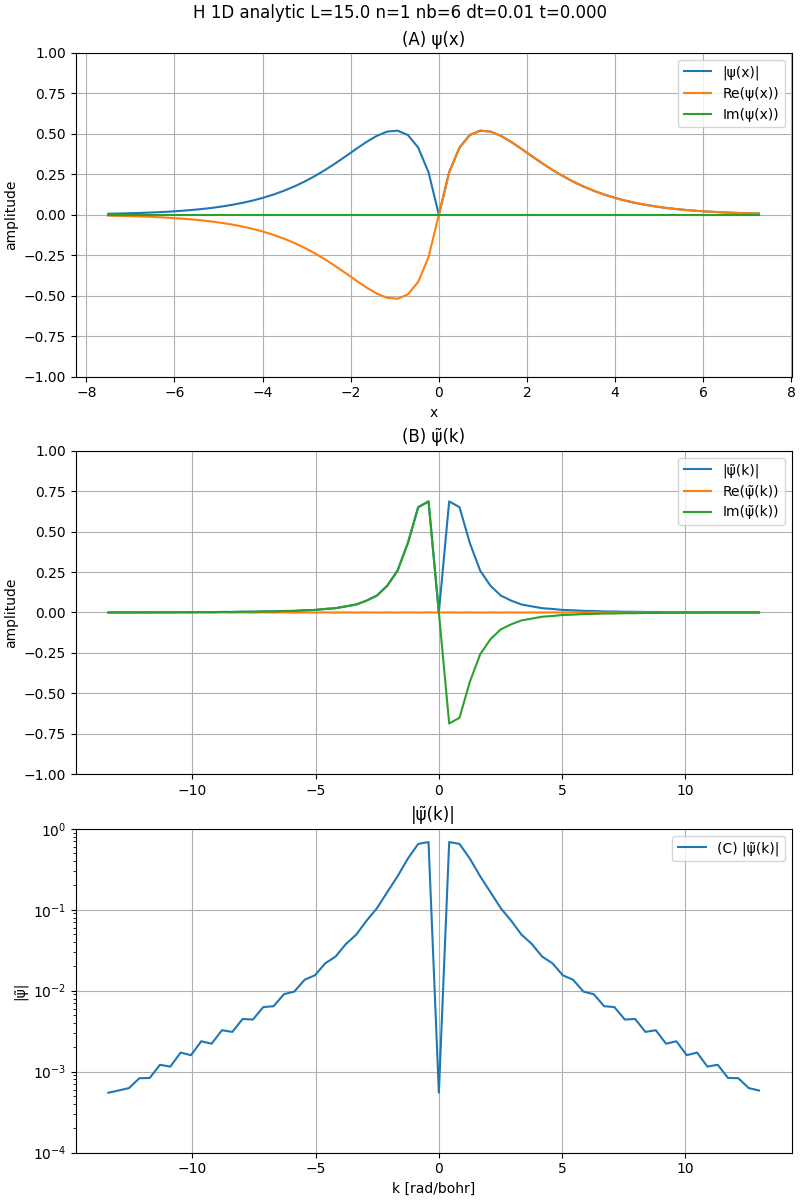
\includegraphics[width=0.6\textwidth]{paper2025_figs/analytic1D/t_00.000.png}
    \caption{1次元モデルの波動関数 $\PsiOneD_1$ の例}
    \label{fig:initial-wavefunction-1d}
    \begin{flushleft}\small

        6ビット分解能での $\PsiOneD_1$ の値(式\eqref{eq:psi1D1-wave-function})。
        (A)はreal-spaceでの波動関数の振幅。(B)はk-spaceでの波動関数の振幅。(C)は
        k-spaceの振幅の対数スケール表示。

    \end{flushleft}
\end{figure}

2次元のモデル$\psi_{n,\ m}^{\mathrm{2D}}$は、Parfittによる解析解を用いる
\cite{Parfitt2002.10.1063/1.1503868}。このモデルは、クーロンポテンシャル
$-1/\sqrt{x^2+y^2}$の下で運動する電子を2次元平面上に拘束したモデルである。波動
関数は二つの量子数 $n\in\{0,\ldots\}, m\in\{-n,\ldots,0,\ldots,n\}$ をパラメータ
として持つ。
\begin{equation}
\psi_{n,\ m}^{\mathrm{2D}}(r,\ \theta)=
\sqrt{\frac{q_0^3(n-\abs{m})!}{\pi(n+\abs{m})!}}(2q_0r)^{\abs{m}}
e^{-q_0r}L_{n-\abs{m}}^{2\abs{m}}(2q_0r)e^{im\theta}
\end{equation}
ここで $q_0=1/(n+1/2)$ である。このエネルギー固有値は量子数$n\in\{0,\ldots\}$を用いて
\begin{equation}
E_n^{\mathrm{2D}}=-\frac{1}{2(n+1/2)^2}
\end{equation}
で与えられる。評価には基底状態$\psi_{0,0}^{2D}$と励起状態$\psi_{1,0}^{2D}$と
$\psi_{1,1}^{2D}$を用いる。
\begin{align}
\psi_{0,0}^{\mathrm{2D}}(r,\theta)&=\sqrt{\frac{8}{\pi}}e^{-2r}
\label{eq:psi2D00-wave-function}\\
E_0^{\mathrm{2D}}&=-2
\label{eq:psi2D00-energy}\\
\psi_{1,0}^{\mathrm{2D}}(r,\theta)&=\sqrt{\frac{8}{27\pi}}(1-\frac{4}{3}r)e^{-\frac{2}{3}r} 
\label{eq:psi2D10-wave-function}\\
\psi_{1,1}^{\mathrm{2D}}(r,\theta)&=\frac{8}{9\sqrt{3\pi}}re^{-\frac{2}{3}r+i\theta}
\label{eq:psi2D11-wave-function}\\
E_1^{\mathrm{2D}}&=-\frac{2}{9}\simeq -0.2222
\label{eq:psi2D10-energy}
\end{align}

$\psi_{0,0}^{\mathrm{2D}}, \psi_{1,0}^{\mathrm{2D}}, \psi_{1,1}^{\mathrm{2D}}$
の位置座標表示と波数表示をそれぞれ図\ref{subfig:initial-wavefunction-2d-0-0},
\ref{subfig:initial-wavefunction-2d-1-0}, \ref{subfig:initial-wavefunction-2d-1-1}  に
示す。

\begin{figure}[ht]
    \centering
    \begin{subfigure}{.45\columnwidth}
        \centering
        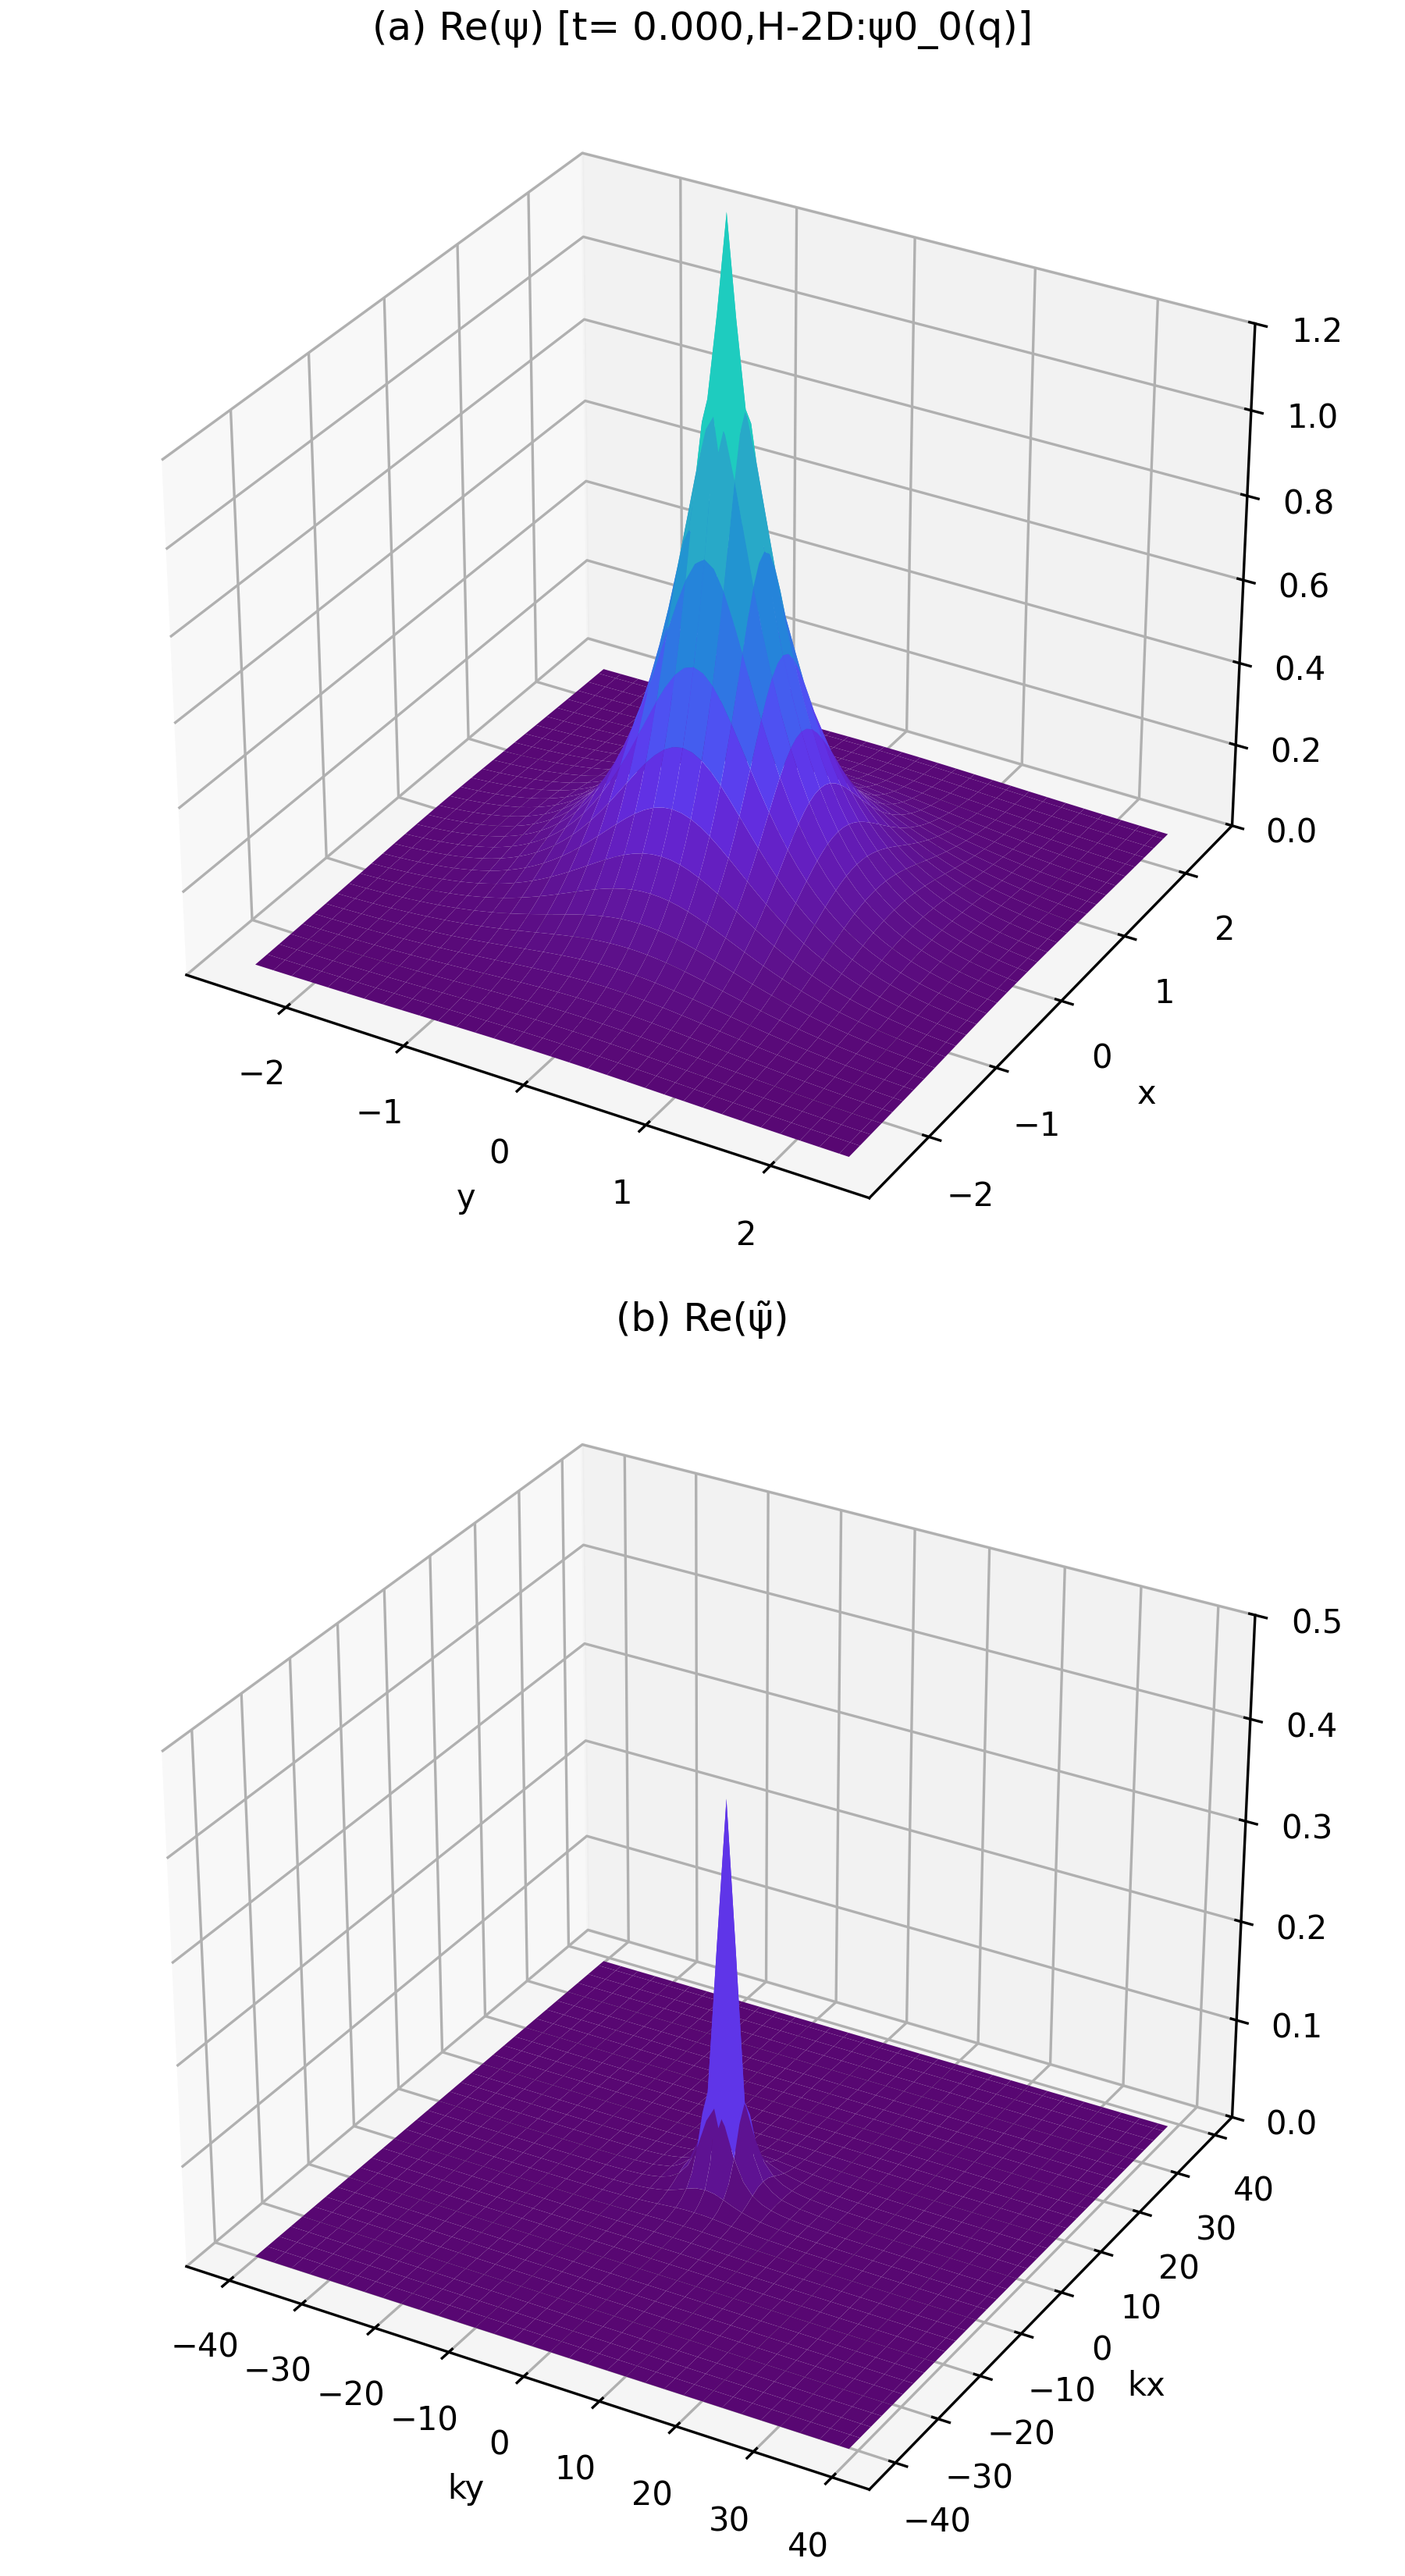
\includegraphics[width=1\columnwidth]{paper2025_figs/classic2D/6b_n0_m0/t_00.000_3d-qp.png}
        \caption{波動関数 $\PsiTwoD_{0,0}$}
        \label{subfig:initial-wavefunction-2d-0-0}
    \end{subfigure}
    \begin{subfigure}{.45\columnwidth}
        \centering
        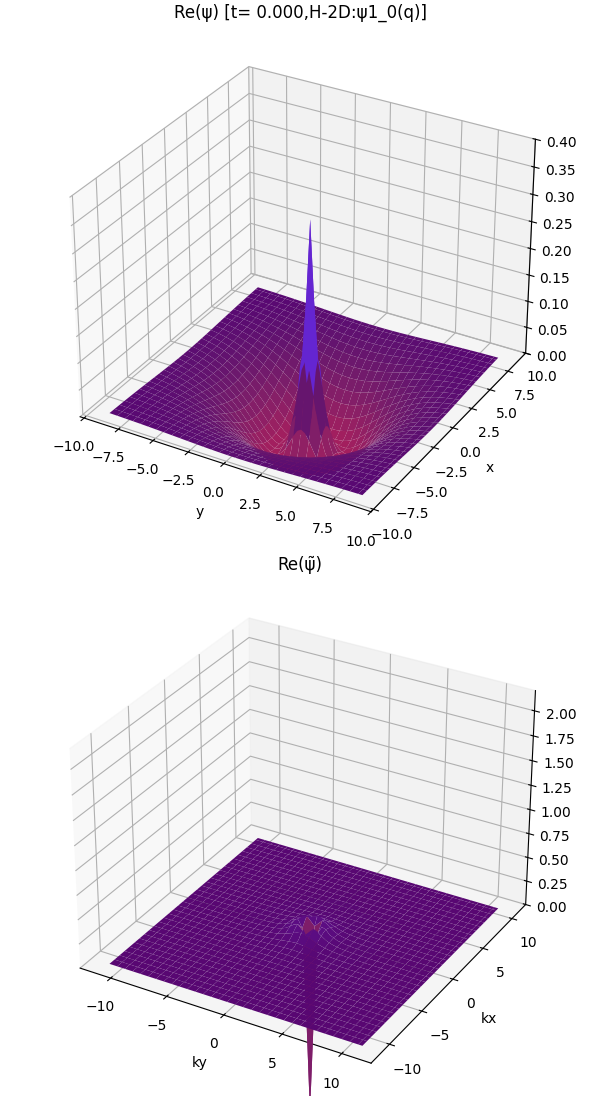
\includegraphics[width=1\columnwidth]{paper2025_figs/classic2D/6b_n1_m0/t_00.000_3d-qp.png}
        \caption{波動関数 $\PsiTwoD_{1,0}$}
        \label{subfig:initial-wavefunction-2d-1-0}
    \end{subfigure}
    \begin{flushleft}\small 

        (a) 主量子数$n=0$ 方位量子数 $m=0$ の基底状態 $\PsiTwoD_{0,0}$(式
        \ref{eq:psi2D00-wave-function})。 (b) $n=1,m=0$ の励起状態
        $\PsiTwoD_{1,0}$ (式\eqref{eq:psi2D10-wave-function})。それぞれ上段が
        real-spaceでの波動関数の実部の値で、下段はk-spaceでの実部の値。(a)と(b)
        は原点での波動関数の値が非ゼロである。

    \end{flushleft}
\end{figure}

\begin{figure}[ht]
    \centering
    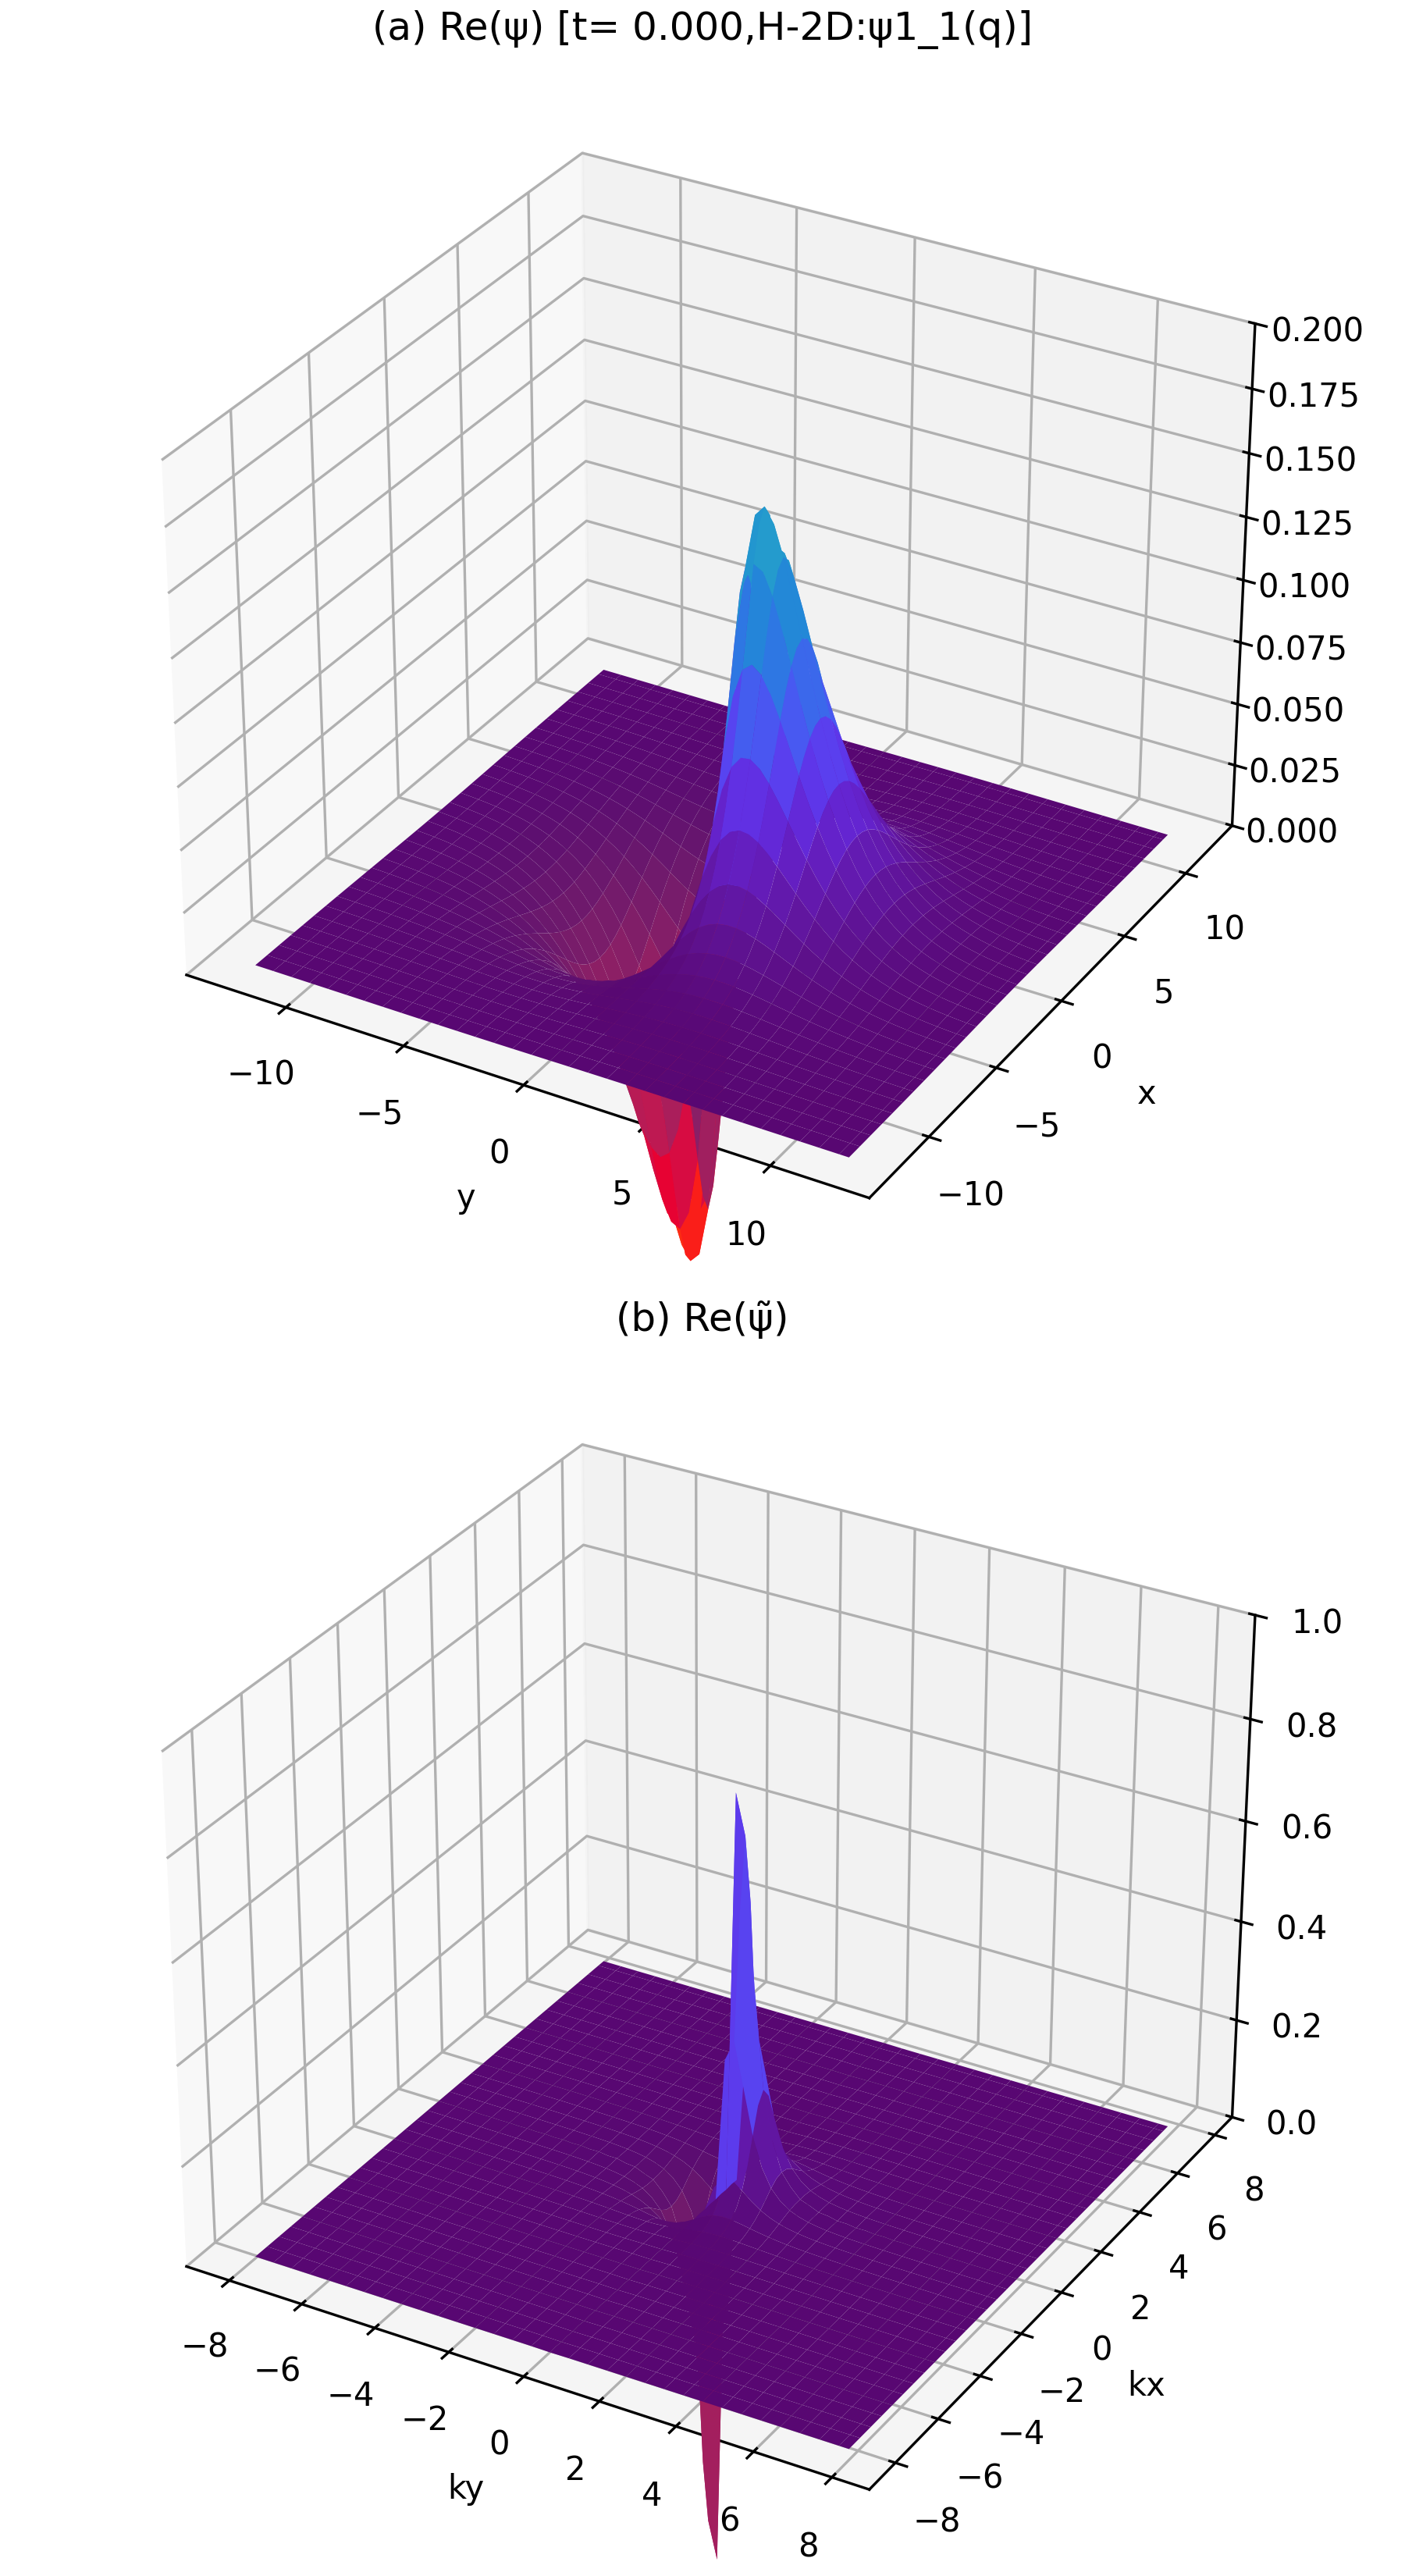
\includegraphics[width=0.45\columnwidth]{paper2025_figs/classic2D/6b_n1_m1/t_00.000_3d-qp.png}
    \caption{波動関数 $\PsiTwoD_{1,1}$}
    \label{subfig:initial-wavefunction-2d-1-1}
    \begin{flushleft}\small

        $n=1,m=1$ の励起状態 $\PsiTwoD_{1,1}$ (式
        \ref{eq:psi2D11-wave-function})。それぞれ上段がreal-spaceでの波動関数の
        実部の値で、下段はk-spaceでの実部の値。原点での波動関数の値がゼロであ
        る。

    \end{flushleft}
\end{figure}


\clearpage
\subsection{古典プログラムによる時間発展シミュレータの併用}
本研究のシミュレータ回路を量子コンピュータのエミュレータ上で動作させるには、回路
のqubit数とゲート数をエミュレータで扱える範囲に抑える必要がある。そのため、指定
できるモデルのパラメータの範囲は限られている。エミュレータで実行可能なパラメータ
の範囲を超える値について評価するために、シミュレータ回路と等価な動作をするように
作成した古典プログラムを併用する。シミュレータ回路で実際に動作させたパラメータに
ついては第\ref{subsec:circuit-size-evaluation}節の表
\ref{tab:emulator-circuit-configurations}に示す。

\subsection{量子コンピュータエミュレータの使用}
本研究では量子回路を実行するのに量子コンピュータの実機ではなく、古典コンピュータ
上の量子コンピュータエミュレータを使用する。これは古典コンピュータ上で動くプログ
ラムであり、量子回路のSDKのツールの一つとして提供されている
\cite{website:qiskit-aer}。

量子コンピュータエミュレータはqubitの状態ベクトルの内容を古典コンピュータのメモ
リ上に保持し、qubitに対する演算については、重ねあわされた個々の状態に対する演算
に展開して実行する。

qubitの状態の表現方法にはいくつか方法があり、最も単純なstate vector法ではqubit数
$N$の状態ベクトルを、要素数$2^N$の配列としてメモリ上に保持する方法である。

qubitの量子もつれの程度が低く、遠く離れたqubit同士のもつれがほとんどない場合に
は、qubitを数珠繋ぎのような行列の連なりとして表現することでメモリ使用量を大幅に
圧縮する、Matrix Product State (MPS)法が知られており、Qiskitのエミュレータでも提
供されている\cite{Vidal2003.PhysRevLett.91.147902}。しかし、第一量子化における
qubitの使い方では、補助qubitを除いて全てのqubitを基本的にもつれさせるので、MPS法
によるデータ圧縮は望めない。そのため、本研究ではstate vector法を用いる。

また、エミュレータの機能として、量子コンピュータ実機のノイズモデルのシミュレー
ションがあるが、本研究のアルゴリズムは演算回数が多いため、ノイズが克服された
Fault Tolerant Quantum Computer(FTQC)での動作が前提となる。そのため回路設計とし
てノイズ影響下での動作を考慮していない。エミュレータを利用する際にはノイズをゼロ
とした理想的な量子コンピュータとして動作させている。


\subsection{使用した計算環境}
シミュレーション計算に使用した計算機ハードウェアとソフトウェアは以下の通りである。
\begin{itemize}
    \item CPU:AMD Ryzen 9 7950X 16 Core × 1
    \item メモリ: 128GB
    \item GPU: NVIDIA GeForce RTX 4090 × 1
    \item OS: Ubuntu 22.04.4 LTS
    \item Quantum SDK: Qiskit 1.4.0, qiskit-aer-gpu 0.15.1
    \item 量子化学シミュレータソフトウェア: Chemical Reaction Simulator Q (crsQ) \cite{website:crsq}
\end{itemize}


\section{限られたqubit数の下でのポテンシャルの計算の工夫}
今後期待される誤り訂正を有するQCは初期においては、誤り訂正技術が必要とする大量の
冗長ビットのために利用可能なqubit数が厳しく限られるであろう。現在利用可能な古典
コンピュータ上のQCエミュレータでも、qubit数の指数のオーダーのメモリと計算量を必
要とするという理由でやはり利用可能なqubit数は厳しく制限される。

量子化学シミュレーションの量子回路が必要とするqubit数やゲート数を見積もる一般的
なアプローチでは計算を希望する分子モデルのサイズと許容する誤差から出発して、それ
に対応するために必要なqubit数とゲート数を見積もるが、本報告では逆に、利用可能な
qubit数から出発して、その上で動作可能な回路構成例を定める方法を検討する。そのた
めに、小規模モデルにおける具体的な規模数値に着目し、大規模モデルに対しては必ずし
も効率的ではない回路構成も取り上げる。

シミュレータ回路の回路規模の主要な部分がクーロンポテンシャルの計算回路である。
Trotter分解に基づく基本的なクーロンポテンシャルの計算回路では、シミュレーション
対象の直方体空間を等間隔の格子に分割し、格子のインデクスを複数のqubitからなるレ
ジスタに対応させ、qubitの値に対する算術演算によりクーロンポテンシャルを計算する
\cite{Zalka-rspa.1998.0162}。算術演算には二進の演算回路を用いる
\cite{Vedral1996.PhysRevA.54.147}。このように構成された回路の規模は、粒子数の多
項式の量子ビット数とゲート数であり、古典計算機よりも指数的に効率がよい。

これが基本となる計算方法である。ただし、オーダーとしては効率的であるものの、必要
な補助qubitの数とゲート数の定数係数は決して小さくはない。

ゲート数を削減する工夫としては$1/\sqrt{x}$の近似値をQROMで求めた後に、
$1/\sqrt{x}$を3次多項式で近似し、Newton-Raphson法で近似値の精度を高める方法が
提案されている\cite{Rubin2024.pnas.2317772121}。

本研究では新たに、ゲート数の増加は許容しても補助qubit数を削減する方法を検討した。

本節では上記の3つの方法について紹介し、1つ目と3つ目の方法については実際に回路と
して実装して評価する。

\subsection{算術演算ゲートによるポテンシャルの計算回路}
\label{subsec:potential-circuit-by-arithmetic-gates}

クーロンポテンシャル計算回路の基本となるのは算術演算回路に基づく方法である
\cite{Zalka-rspa.1998.0162}。

\begin{figure}[ht]
    \centering
    \begin{quantikz}[transparent]
        \lstick{$n_1$} & \qwbundle{\nb} & \gate[4]{\Thetaep} &                   & \gate[4]{\Thetaep} &\\
        \lstick{$n_2$} & \qwbundle{\nb} &                    &\gate[3]{\Thetaep} & \linethrough &\\
        \lstick{$n_3$} & \qwbundle{\nb} & \linethrough       &                   & & \\
        \lstick{$tmp$} & \qwbundle{} &                    &                   & &
    \end{quantikz}

    \caption{3電子系におけるクーロンポテンシャル項回路 $\Thetaep$ の例}
    \label{fig:theta-ep-multi-electron}
    \begin{flushleft}\small
        
        $n_1,n_2,n_3$はそれぞれ電子 1,2,3 の離散化された座標に対応するレジスタで
        あり、それぞれ$\nb$ビットからなる。qubitの線に付けられた斜線はその線が単
        一のqubitではなく複数のqubitからなるレジスタであることを示す。 $tmp$は補
        助qubitレジスタである。クーロンポテンシャル計算回路$\Thetaep$は3組の電子
        対 (1,2), (2,3), (1,3) のそれぞれに対して設ける必要があるが、補助qubitレ
        ジスタは1組だけでよい。$\Thetaep$回路の箱を貫通しているqubitの線はその回
        路がそのqubitを使用しないことを示す。
    \end{flushleft}
\end{figure}

この回路では計算途中の値を保持するための補助qubitを相当数必要とするが、多数の粒
子からなる系を扱う場合、粒子対の数の分だけ演算回路が必要となるものの、異なる粒子
対に対する計算に対して一組の補助qubitを繰り返し使うことができるので、図
\ref{fig:theta-ep-multi-electron}に示すように粒子数が増えても補助qubitの数を一定
に保つことができる。そのため、回路のqubit数の粒子数に対する依存性の評価において
は一般的に補助qubitの数自体は問題視されない。しかし、小規模モデルにおいては補助
qubitの個数が回路のqubit数の相当な割合を占める。

図\ref{subfig:circuit-1d-arith-overall}は算術演算回路を用いたシミュレータ回路の
全体像である。シミュレータ回路は、状態準備回路と時間発展回路から構成される。時間
発展回路のqubit数が支配的であることが分かる。

図\ref{subfig:circuit-1d-arith-time-evolution}は時間発展回路$\Thetae$の内部の回
路を示している(式\eqref{eq:circuit-eval-theta-e})。時間発展回路はクーロンポテン
シャルエネルギー項回路 $\Thetaep$、逆QFT回路、運動エネルギー項回路
$\Thetaek$、QFT回路から構成される。図
\ref{subfig:potential-energy-circuit-1d-arith}は $\Thetaep$ を示している。この回
路は$1/|x|$を計算する回路である。

\begin{figure}[ht]
    \centering
    \begin{subcaptionblock}[T][][t]{0.3\columnwidth}
        \centering
        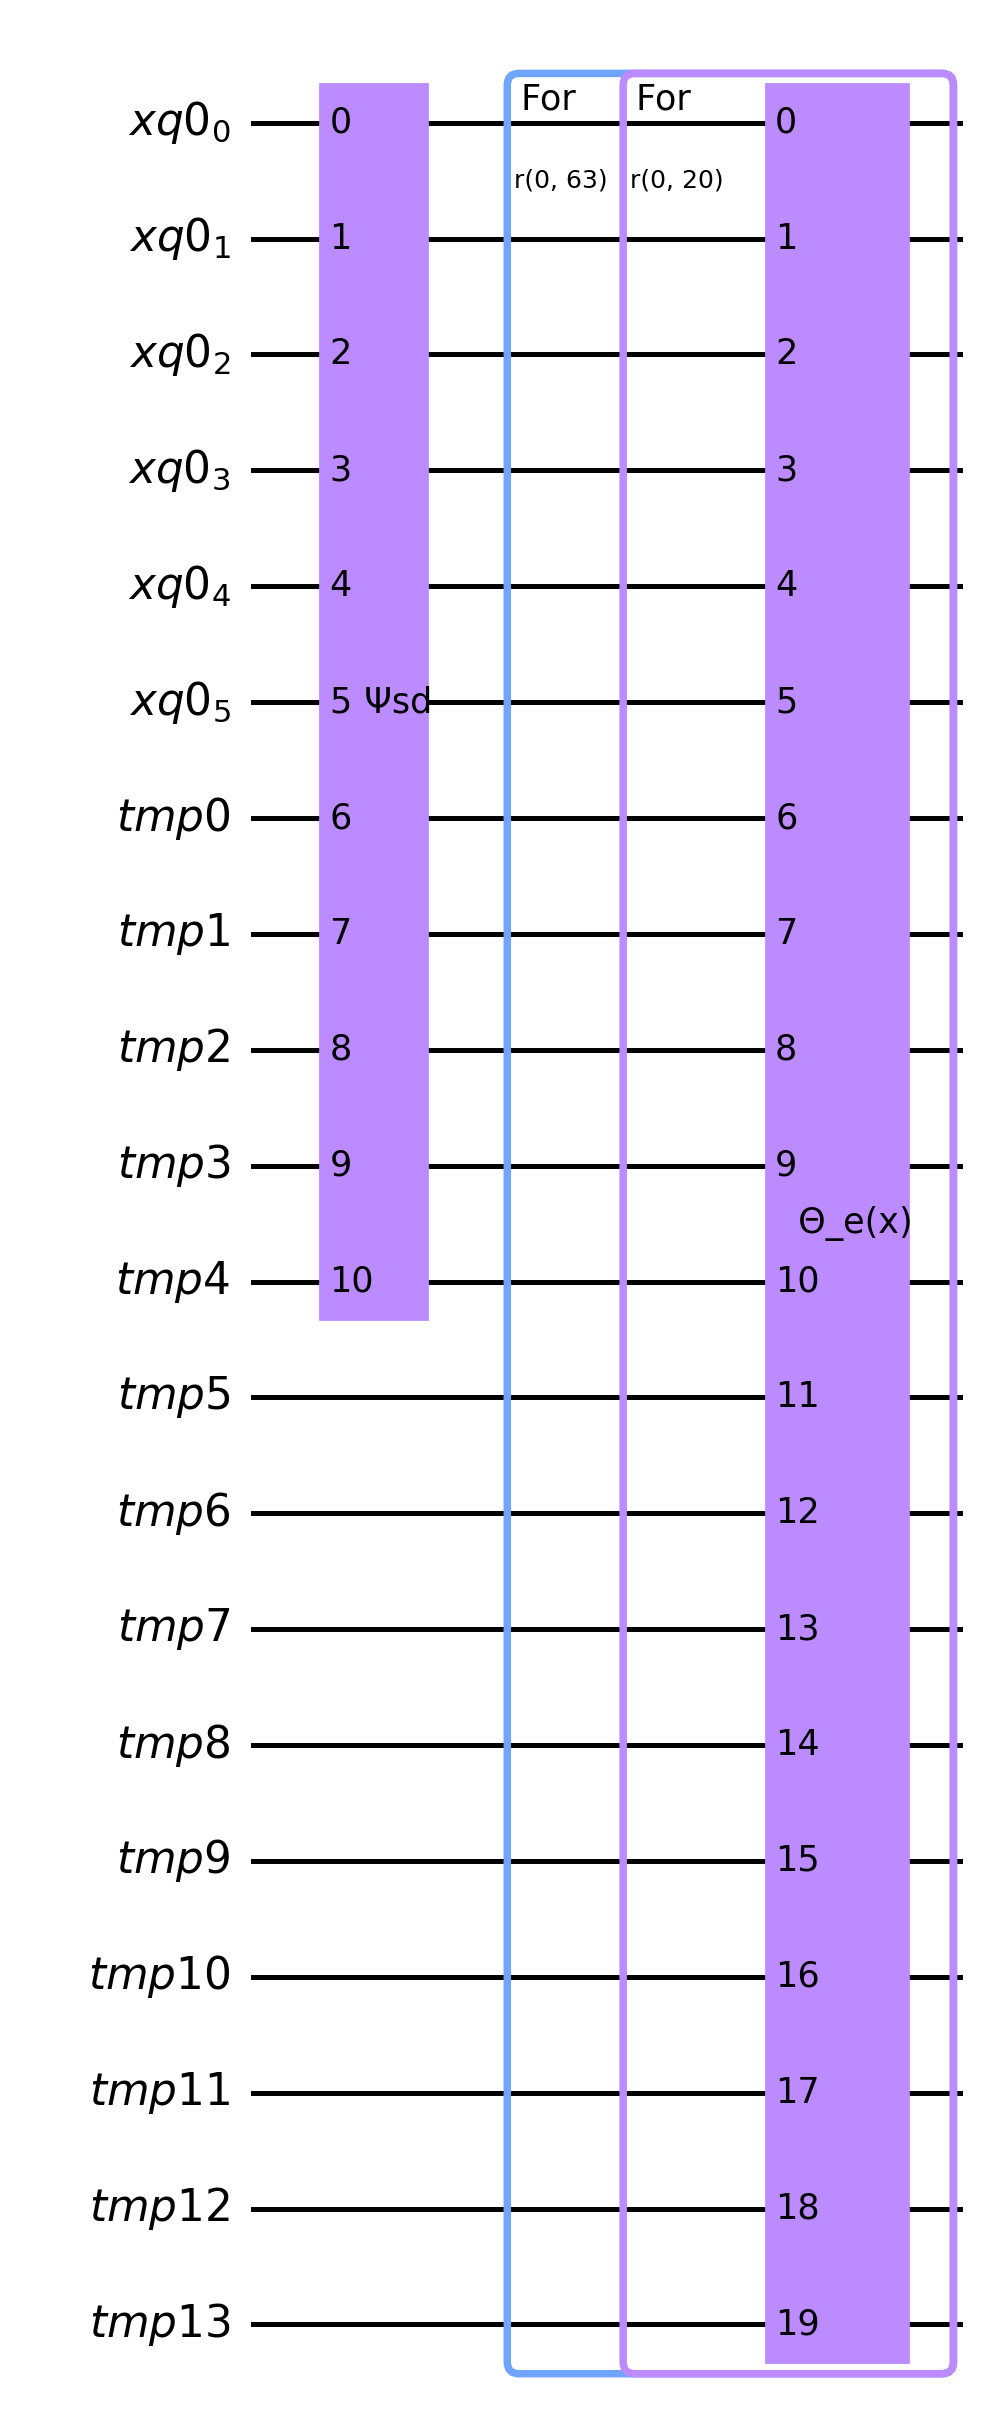
\includegraphics[width=\textwidth]{paper2025_figs/arith1D/circuit.png}
        \caption{回路の全体像}
        \label{subfig:circuit-1d-arith-overall}
    \end{subcaptionblock}
    \begin{subcaptionblock}[T][][t]{0.42\columnwidth}
        \centering
        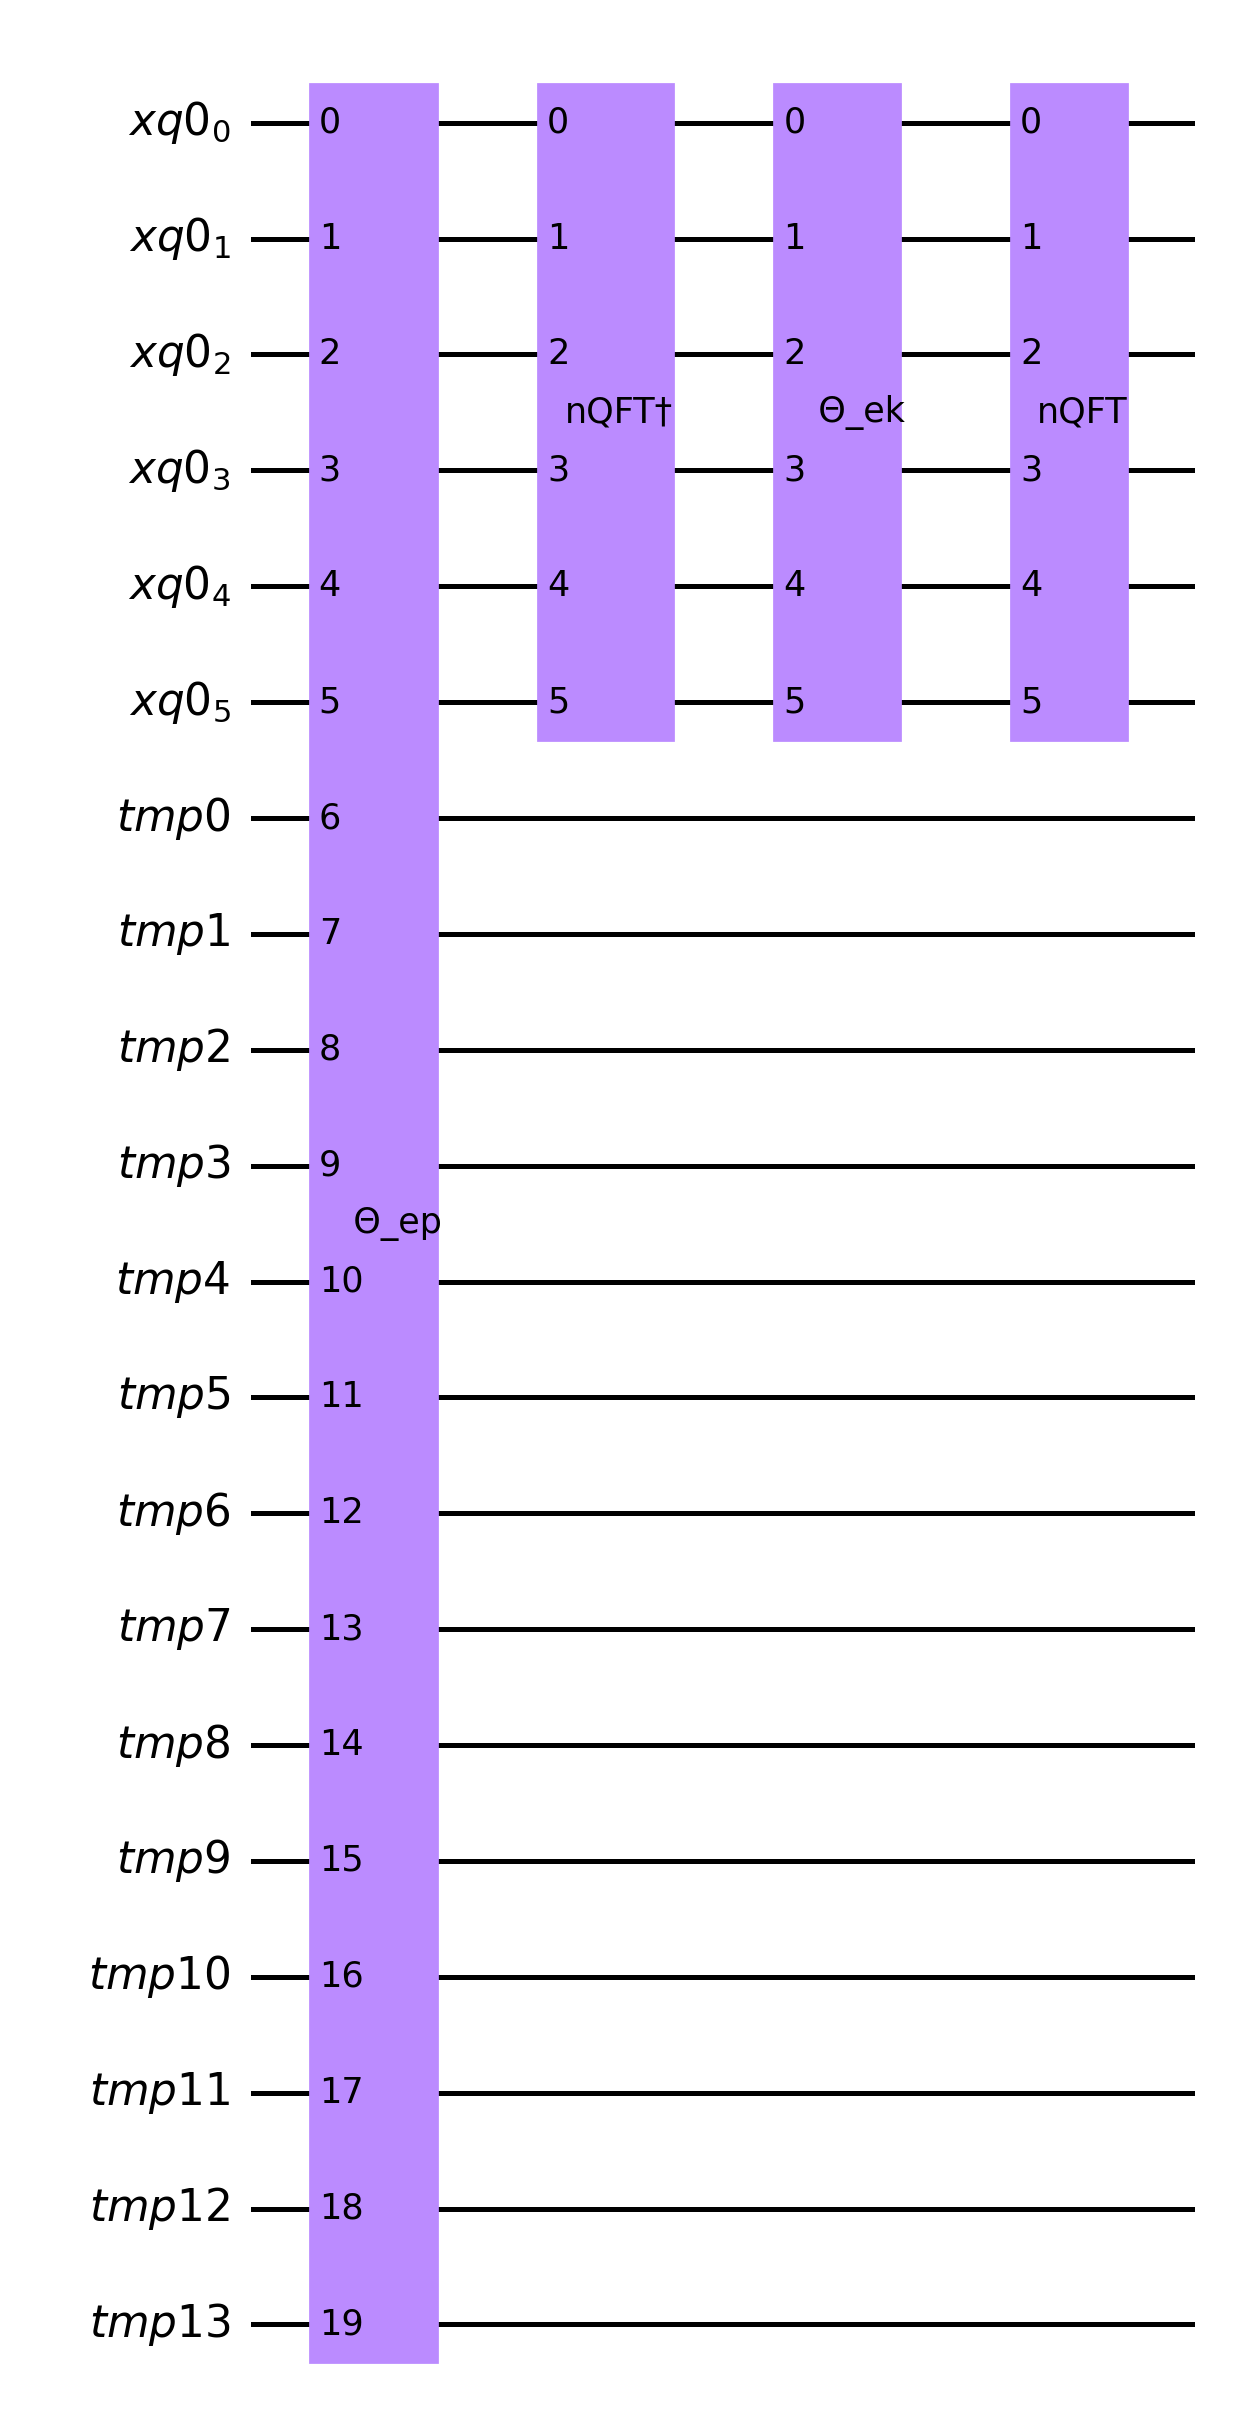
\includegraphics[width=\textwidth]{paper2025_figs/arith1D/elec_motion.png}
        \caption{時間発展回路$\Thetae$の内部}
        \label{subfig:circuit-1d-arith-time-evolution}
    \end{subcaptionblock}
    \caption{算術演算ゲートによる1次元モデルのシミュレータ回路}
    \label{fig:circuit-1d-arith}
    \begin{flushleft}\small

        (a)は1次元モデルのシミュレータ回路の全体像を示す。回路は初期化回路
        $\PsiSD$と時間発展回路$\Thetae$から構成される。(b)は時間発展回路
        $\Thetae$の内部構成を示している。ポテンシャルエネルギー項回路
        $\Thetaep$、逆QFT回路、運動エネルギー項回路$\Thetaek$、QFT回路から構成さ
        れる。 $\Thetaep$のqubit数23が回路全体のqubit数を規定している。

    \end{flushleft}
\end{figure}

\begin{figure}[ht]
    \centering
    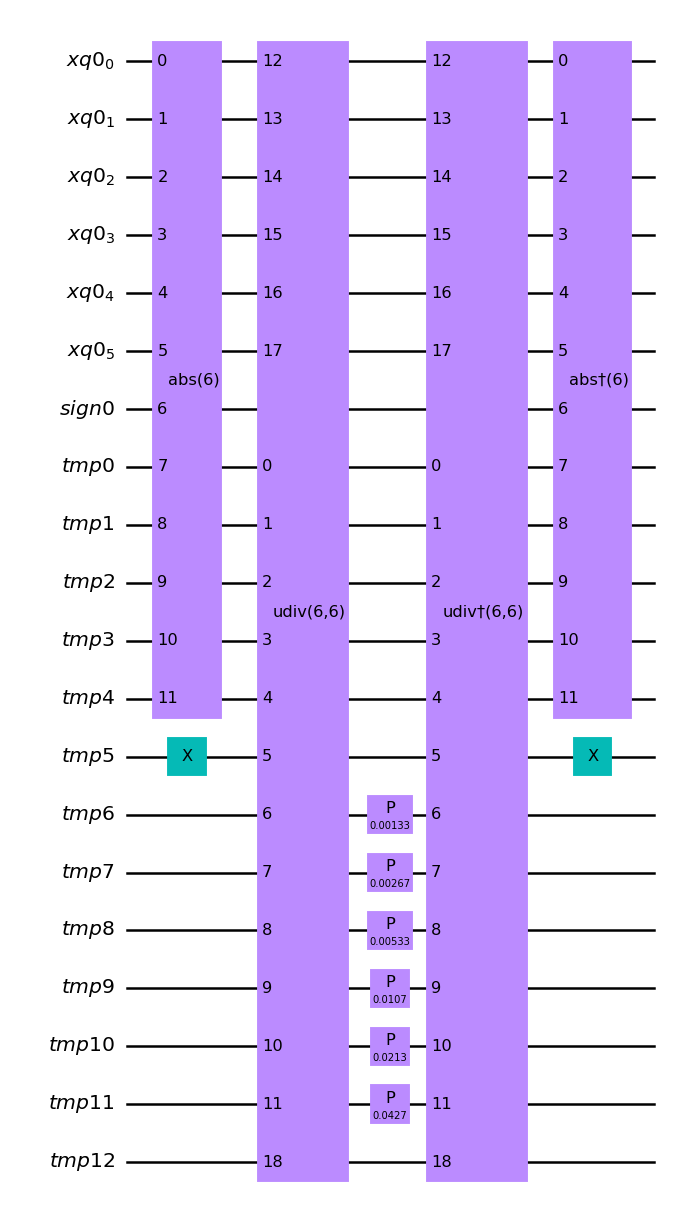
\includegraphics[width=0.5\textwidth]{paper2025_figs/arith1D/elec_potential_arithmetic.png}
    \caption{算術演算ゲートによるポテンシャルエネルギー項回路 $\Thetaep$}
    \label{subfig:potential-energy-circuit-1d-arith}
    \begin{flushleft}\small

        算術演算ゲートを用いて実装されたクーロンポテンシャル項回路$\Thetaep$回路
        の中身。算術演算ゲートで $1/|x|$を2進数で計算し、結果のビット列の各ビッ
        トの重みに応じてPゲートで位相を変化させている。除算ゲートudiv7のqubit数
        が支配的である。補助qubitの総数は17ビットである。

    \end{flushleft}
\end{figure}
\clearpage
\subsection{QROMとNewton-Raphson法を併用するポテンシャルの計算回路}
\label{subsec:potential-circuit-by-qrom-newton-raphson}

第一量子化の時間発展シミュレーションの先行研究では、qubit数の定数因子については
受容している一方でゲート数については削減が模索されている。例えば、ゲート数の多い
平方根と除算を合わせて回避する改良案としてはQuantum Read Only Memory (QROM)で概
算値を求めてからNewton-Raphson法を1ステップ実行することで精度を高める方式が提案
されている\cite{Rubin2024.pnas.2317772121}。この方法では、$1/\sqrt{x}$を3次多項
式で近似し、 Newton-Raphson法を用いて解を求める。精度を高めるために、計算の定義
域を区画に分割して区画ごとに3次多項式の係数を変える。また、Newton-Raphson法を1ス
テップだけで済ませるために、$1/\sqrt{x}$の近似値をQROMで与える。QROMの元々の提案
では、 QROM回路は入力ビットの指数のゲート数を必要とする
\cite{Babbush_2018b.PhysRevX.8.041015}。しかしここでは
\cite{Sanders2020.PRXQuantum.1.020312}で提案されたVariable Spacingという手法を用
いて、QROM回路のゲート数をビット数のオーダーまで抑えている。

この方法では平方根と除算の回路を回避できるため、ゲート数を削減することができる
が、 QROM回路が必要とする補助qubit数は依然として多い。QROM回路は出力ビット数に比
例した補助qubit数を必要とするためである。そのため、小規模モデルにおいては補助
qubit数が回路全体のqubit数に占める割合が大きくなり、回路全体のqubit数の削減には
寄与しない。粒子数がある程度多い大規模モデルにおいて有効な方法である。

この方式は必要とするqubit数が多く、エミュレータによる動作が困難であるため、本研
究においてはこの方法の実装はしていない。

\subsection{UCRZゲートによるポテンシャルの計算回路}
\label{subsec:potential-circuit-by-ucrz-qubits}

本研究では、電子数が少ないモデルのシミュレーションを扱うため定数個の補助qubit数
も問題視し、これを削減する手段としてQROMと作用が似ている回路であるUniformly
Controlled Rotation (UCR)回路に着目する
\cite{Mottonen2004.PhysRevLett.93.130502}。UCR回路のバリエーションのひとつ、UCRZ
回路では回路の出力がターゲットとするqubitの位相回転角として得られる。これはクー
ロンポテンシャル回路の出力と形式が同じであるので、UCRZ回路の出力をクーロンポテン
シャル回路の出力としてそのまま使うことができる。UCRZ回路が必要とする補助qubit
は、ターゲットqubit一つだけであるので、算術演算回路に比べて補助qubitを大幅に減ら
すことができる。ただし、この回路のゲート数はQROM回路と同様にコントロールレジスタ
の指数となるので、大規模なモデルへの適用は現実的ではないが、小さいモデルにおいて
は有効な選択肢となる。UCRZ回路は総qubit数が限定されている場合の代替の回路として
有用である。本研究ではUCRZ回路を用いることによって2次元モデルの計算がエミュレー
タ上で実行可能となった。

UCR回路は$n$ビットの入力レジスタの値のビット列に応じて単一のターゲットqubit $t$
に特定の回転軸$a$ まわりの回転を与える回路である
\cite{Mottonen2004.PhysRevLett.93.130502}。入力値に対して事前に指定された値を出
力するという点で、UCR回路の働きはQROM回路の一種とみなすことができる。一般のQROM
が出力を出力レジスタ上のビット列として出力するのに対してUCR回路はターゲットqubit
の回転角として出力する。UCRZ回路は出力がターゲットqubitの位相変化であるため、時
間発展演算子のポテンシャル項の計算にそのまま使うことができ、粒子間の距離計算と逆
数計算とを単一のUCRZ回路で置き換えることができる。その結果算術演算回路で必要な多
数の補助qubitを省略することが可能になる。

UCR回路の作用を式で表すと
\begin{equation}
    \ket{b}\ket{t} \mapsto \ket{b} R_{\mathrm{a}}(\theta_{\mathrm{b}})\ket{t}
\end{equation}
となる。

\begin{figure}[ht]
    \centering
    \begin{quantikz}[column sep=0.3cm]
        \lstick{$b_0$} & & \ctrl{3} & &          & & \ctrl{3} & &          & & \ctrl{3} & &          & & \ctrl{3} & &          &\\
        \lstick{$b_1$} & &          & & \ctrl{2} & &          & &          & &          & & \ctrl{2} & &          & &          &\\
        \lstick{$b_2$} & &          & &          & &          & & \ctrl{1} & &          & &          & &          & & \ctrl{1} &\\
        \lstick{$t$} & \gate{\mathrm{R_0}} & \targ{} & \gate{\mathrm{R_1}} & \targ{} & \gate{\mathrm{R_2}} & \targ{} & \gate{\mathrm{R_3}} & \targ{} &
                       \gate{\mathrm{R_4}} & \targ{} & \gate{\mathrm{R_5}} & \targ{} & \gate{\mathrm{R_6}} & \targ{} & \gate{\mathrm{R_7}} & \targ{} &
    \end{quantikz}
    \caption{3ビット入力のUCRZ回路の例}
    \label{fig:ucrz-n3}
    \begin{flushleft}\small 3ビットの入力レジスタ$b_2b_1b_0$に対して8通りの入力
    値があり、それぞれに対応する8個のRzゲートがターゲットqubitに対して作用す
    る。$\mathrm{R}_k$は$\mathrm{Rz}(\theta_k)$を表す。 各Rzゲートは事前に指定
    された回転角$\theta_k$で位相を回転させる。Rzゲートの前後にC-NOTゲートが配置
    されており、入力レジスタのビット列に応じてRzゲートの作用が反転する。
    \end{flushleft}
\end{figure}

$n$ビット入力のUCRZ回路は、ターゲットqubitに対するC-NOTとRzゲートを交互に$2^n$個
並べた回路である。3ビット入力のUCRZ回路の例を図\ref{fig:ucrz-n3}に示す。

$k$番目のRzゲート$\mathrm{R_Z}_k$は事前に決めた角度$\theta_k$
だけ位相を回転させる。全てのC-NOTが反転しない場合、回路全体での回転角は
$\theta_k$ の合計値になる。しかし、反転するC-NOTが存在する場合、反転するC-NOTに挟
まれる全てのRzゲートは$\mathrm{XR_z}(\theta)\mathrm{X}=\mathrm{R_z}(-\theta)$の関係から、回転角の符号が反転する。行列
で表すと
\begin{equation}
    \mathrm{XRz}(\theta)\mathrm{X} = \begin{pmatrix}
        0 & 1 \\
        1 & 0
    \end{pmatrix}
    \begin{pmatrix}
        e^{-i\theta/2} & 0 \\
        0 & e^{i\theta/2}
    \end{pmatrix}
    \begin{pmatrix}
        0 & 1 \\
        1 & 0
    \end{pmatrix}
    = \begin{pmatrix}
        e^{i\theta/2} & 0 \\
        0 & e^{-i\theta/2}
    \end{pmatrix}
    = \mathrm{Rz}(-\theta)
\end{equation}
である。

C-NOTのコントロールビットには入力レジスタ $b$のいずれかのビットがつながれるの
で、 $b$ の値に応じて作用が反転するRzゲートが変わる。その結果、入力 $b$ に対して
出力される回転角の合計値 $\alpha_b$ は$\alpha_b=\sum_{k}{(-1)^{f_k(b)}\theta_k}$
のようになる。すなわち、$\theta_k$ の符号を $k,b$ に応じて決めて加算した値とな
る。$\theta_k$から$\alpha_b$ への写像は逆写像が知られているので、各bに対して所望
の $\alpha_b$ が得られるように$\theta_k$ を定めることができる。

クーロンポテンシャル項回路においては、粒子の座標のqubitをUCR回路の入力qubitの$b$を
通し番号とする格子点$\bm{\chi}_b$に対応させ、その格子点でのポテンシャルエネルギー
$\Hp(\bm{\chi}_b)$に基づいてターゲットqubitの位相回転角$\alpha_b$を
\begin{equation}
\alpha_b = -\frac{\Hp(\bm{\chi}_b)\deltat}{\hbar}
\end{equation}
と指定することで、求める時間発展演算子のポテンシャルエネルギー項回路となる。

図\ref{fig:circuit-2d-ucrz}は水素の2次元モデルに対するUCRZ回路を用いたシミュレー
タ回路である。

\begin{figure}[ht]
    \centering
    \begin{subcaptionblock}[T][][t]{0.3\columnwidth}
        \centering
        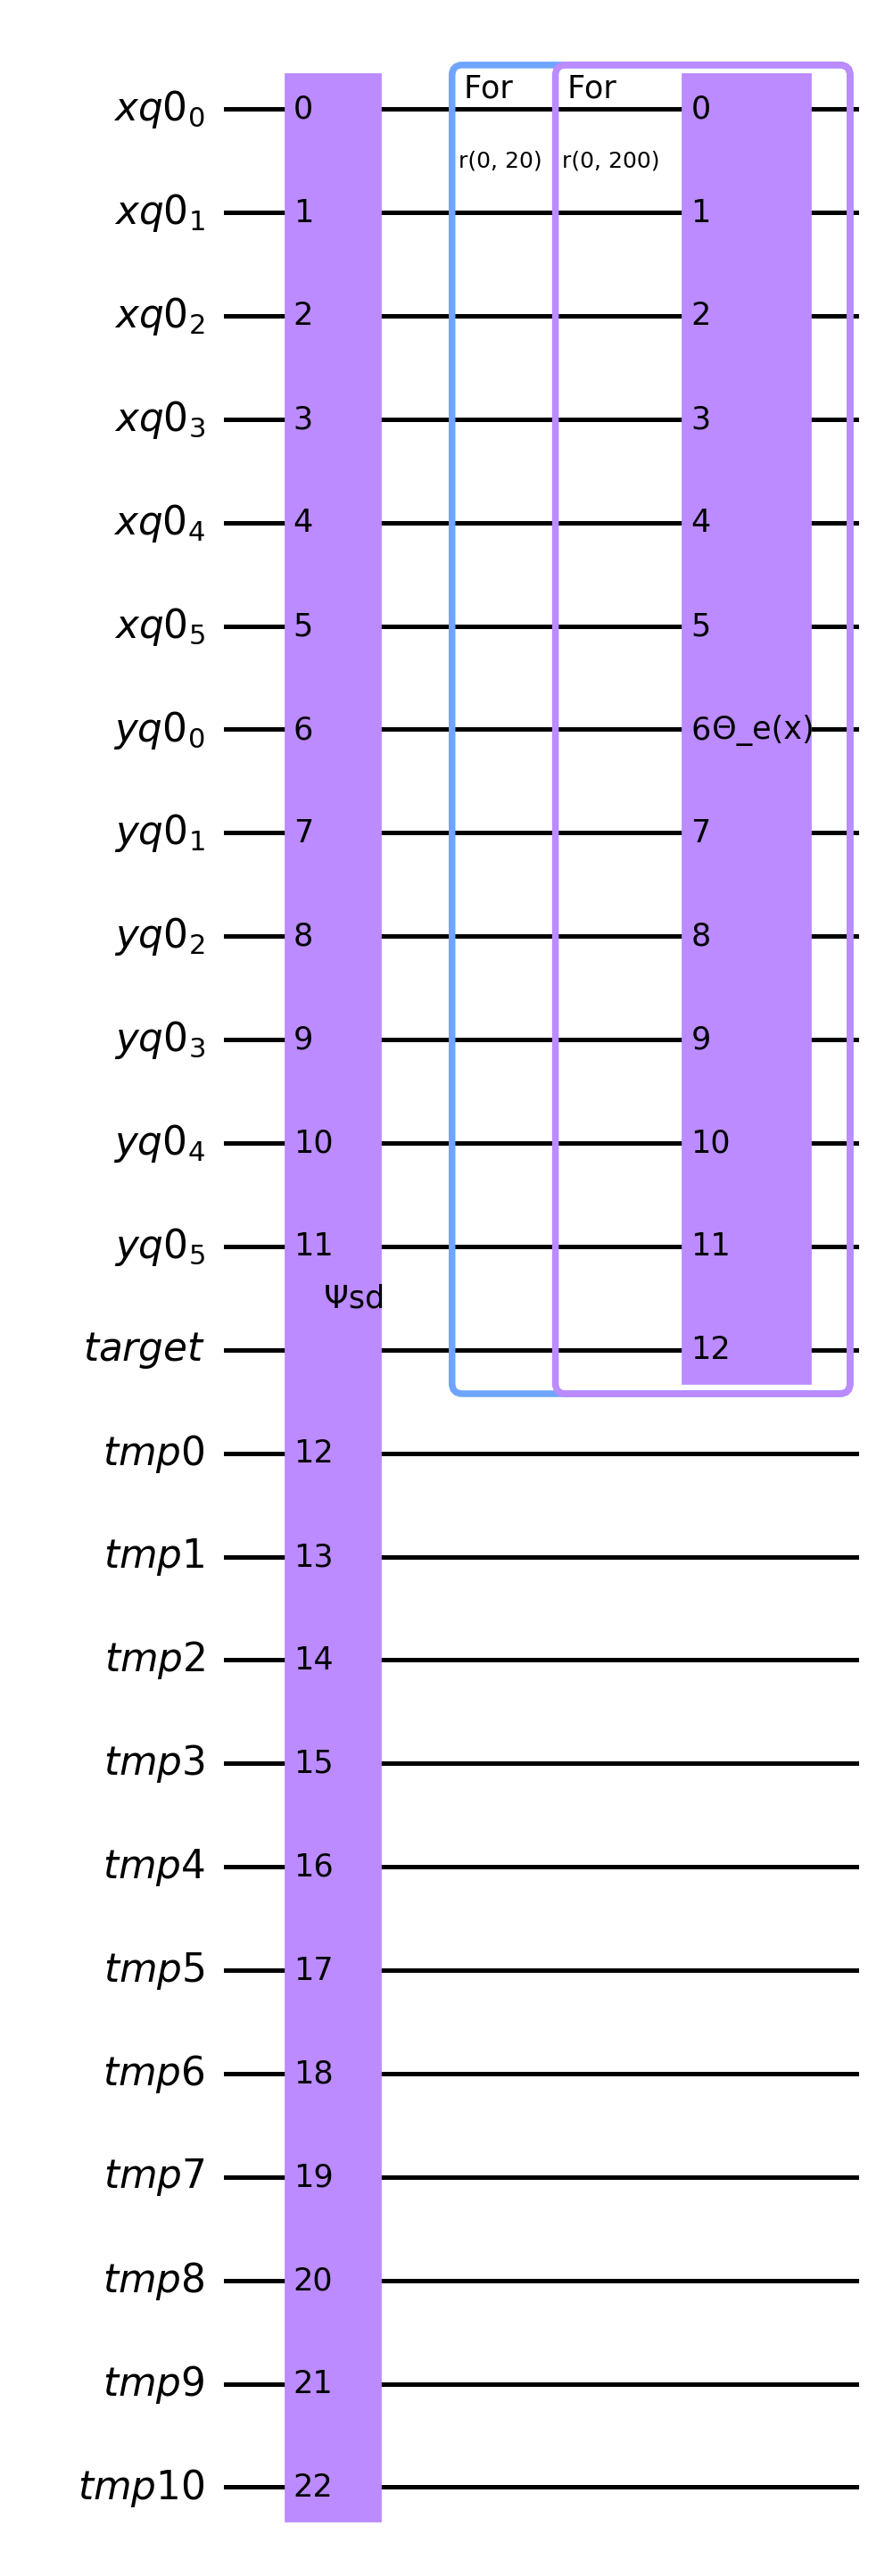
\includegraphics[width=\textwidth]{paper2025_figs/ucrz2D/circuit.png}
        \caption{シミュレータ全体}
        \label{subfig:circuit-2d-ucrz-overall}
    \end{subcaptionblock}
    \begin{subcaptionblock}[T][][t]{0.52\columnwidth}
        \centering
        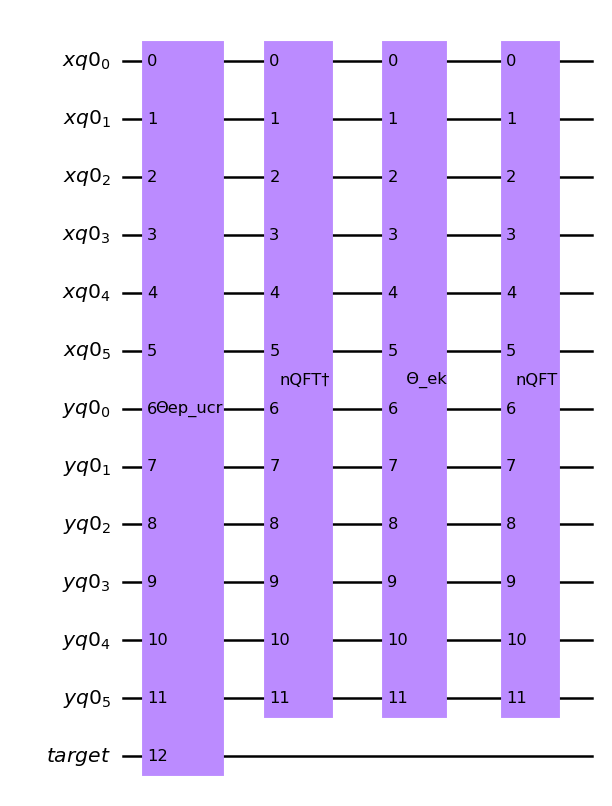
\includegraphics[width=0.8\textwidth]{paper2025_figs/ucrz2D/elec_motion.png}
        \caption{時間発展回路 $\Thetae$ の内部}
        \label{subfig:time-evolution-circuit-2d-ucrz}
    \end{subcaptionblock}
    \caption{UCRZ回路を用いた座標分解能6bit の2次元モデルのシミュレータ回路}
    \label{fig:circuit-2d-ucrz}
    \begin{flushleft}\small

        (a) シミュレータ回路の全体図。状態準備回路と時間発展回路から構成され
        る。qubit数は状態準備回路の方が多い。(B)は時間発展回路の構成であり、ポテ
        ンシャルエネルギー項回路 $\Thetaepucr$ はUniformly controlled Rotation
        (UCR) 回路の一種、UCRZ回路を用いている。この例では6ビットの入力レジスタ
        $xq0$, $yq0$の合計12ビットに与えられた重ねあわされた入力の値のそれぞれに
        応じて補助 qubit である $target$ の位相を変化させる。補助 qubit は$target$
        の1つだけである。
    \end{flushleft}
\end{figure}

\clearpage
\subsection{回路規模の評価}
\label{subsec:circuit-size-evaluation}
今回用いた計算環境のエミュレータで動作させられた最大のqubit数は27、ゲート数の現
実的な上限は$10^7$程度であった。シミュレータの回路を生成させて回路規模を測定するこ
とで、この範囲に回路規模が収まる回路構成を調べた。

\begin{figure}[ht]
    \centering
    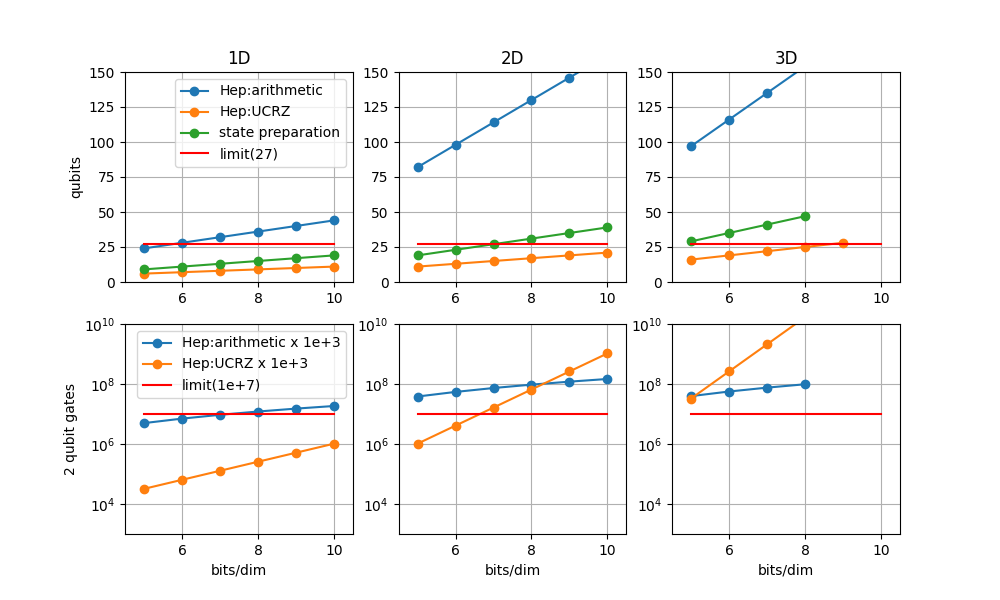
\includegraphics[width=15cm]{paper2025_figs/hamiltonian-gatecount.png}
    \caption{回路規模}
    \label{fig:hamiltonian-gatecount}
    \begin{flushleft}\small
    上段のグラフは1Dから3Dのモデルにおける回路のqubit数を示している。qubit数の多い
    ものから順に、算術演算ゲート版回路、UCRZ版回路、状態準備回路を示している。状
    態準備回路と時間発展回路の双方がqubit数制限に収まっている必要がある。算術演
    算回路がqubit数の上限に収まっているのは1Dの7ビット以下の範囲に限られる。状態
    準備回路が制限に収まっているのは2Dの7ビットのケースまでである。UCRZ回路は3D
    の8ビットのケースまで範囲に収まっている。算術演算ゲートの回路のqubit数が1Dの
    場合と2D,3Dの場合とで大きく異なっているが、これは1Dにおいては距離計算が絶対
    値回路で済むのに対して2D,3Dでは二乗回路と平方根回路を用いたノルム計算が必要
    となり、回路が複雑になるためである。

    下段のグラフは回路が使用するtwo-qubitゲートの数である。時間発展回路のゲート数は
    シミュレーションのステップ数の一例として1000ステップ分の回路のゲート数を示し
    ている。状態準備回路は1回しか実行されないので無視している。算術演算回路の
    ゲート数はどの次元でも大きく値が変わらないがUCRZ回路は傾きが次元に応じて大き
    くなっている。これはUCRZ回路のゲート数が入力ビット数の指数に比例し、入力ビッ
    ト数は次元数×座標ビット数になっているためである。その結果、1次元では常に
    UCRZ回路のゲート数の方が少ないが、3DになるとUCRZ回路のゲート数の方が算術演算
    回路版のゲート数よりも多くなっている。
    \end{flushleft}
\end{figure}

$\Thetaep$ を算術演算ゲートで実装した場合とUCRZゲートで実装した場合とで回路の
qubit数と時間発展1ステップあたりのtwo-qubitゲート数を比較したグラフを図
\ref{fig:hamiltonian-gatecount}に示す。グラフにはさらにシステムの状態準備回路の
値もプロットしている。これらのグラフから、1次元モデルおよび2次元モデルの座標
ビット数6bitまでであればUCRZ回路の方が算術演算回路よりもビット数だけでなくゲート
数も少ないことが分かる。一方で3次元モデルではどのビット数においても算術演算ゲー
ト版のゲート数がUCRZ回路版のゲート数を下回っており、UCRZよりも有利な回路となって
いることが分かる。

量子コンピュータ実機で回路を動作させる場合には、ビット数とモデルの次元数に応じて
有利な回路構成を選ぶことが推奨できる。

\clearpage

\begin{table}[ht]
\centering
\caption{エミュレータで動作した回路構成一覧}
\begin{tabular}{r|c|c}
    \hline
    次元数 & 算術ゲート版回路の$\nb$ & UCRZ版回路の$\nb$ \\
    \hline
    1 & 6,7 & 評価せず \\
    2 & 動作せず & 6 \\
    3 & 動作せず & 動作せず \\
    \hline
\end{tabular}
\label{tab:emulator-circuit-configurations}
\end{table}

次元数1から3のそれぞれにおいて動作可能であった回路の構成を 表
\ref{tab:emulator-circuit-configurations} に示す。1次元のモデルでは算術演算回路
版のシミュレータが動作可能であったのでUCRZ回路版は評価していない。2次元のモデル
では算術演算回路版は動作できず、UCRZ回路版のみが動作可能であった。3次元のモデル
ではいずれの版の回路も動作不能であった。

1次元、2次元のモデル共に、回路をエミュレータ上で動作させることができた。計算にあ
たっては、第\ref{sec:coulomb-potential-handling}節で述べるクーロンポテンシャルの
特異点の扱い方を採用し、第\ref{sec:parameter-selection-for-minimum-error}節で述
べる誤差最小化のためのパラメータ選択を行った。これにより、算術演算ゲートを用いた
クーロンポテンシャル計算回路、UCRZ回路によるクーロンポテンシャル計算回路共に、期
待する波動関数の時間発展動作を得ることができた。計算の誤差については第
\ref{sec:parameter-selection-for-minimum-error}節で分析する。

\begin{figure}[ht]
    \centering
    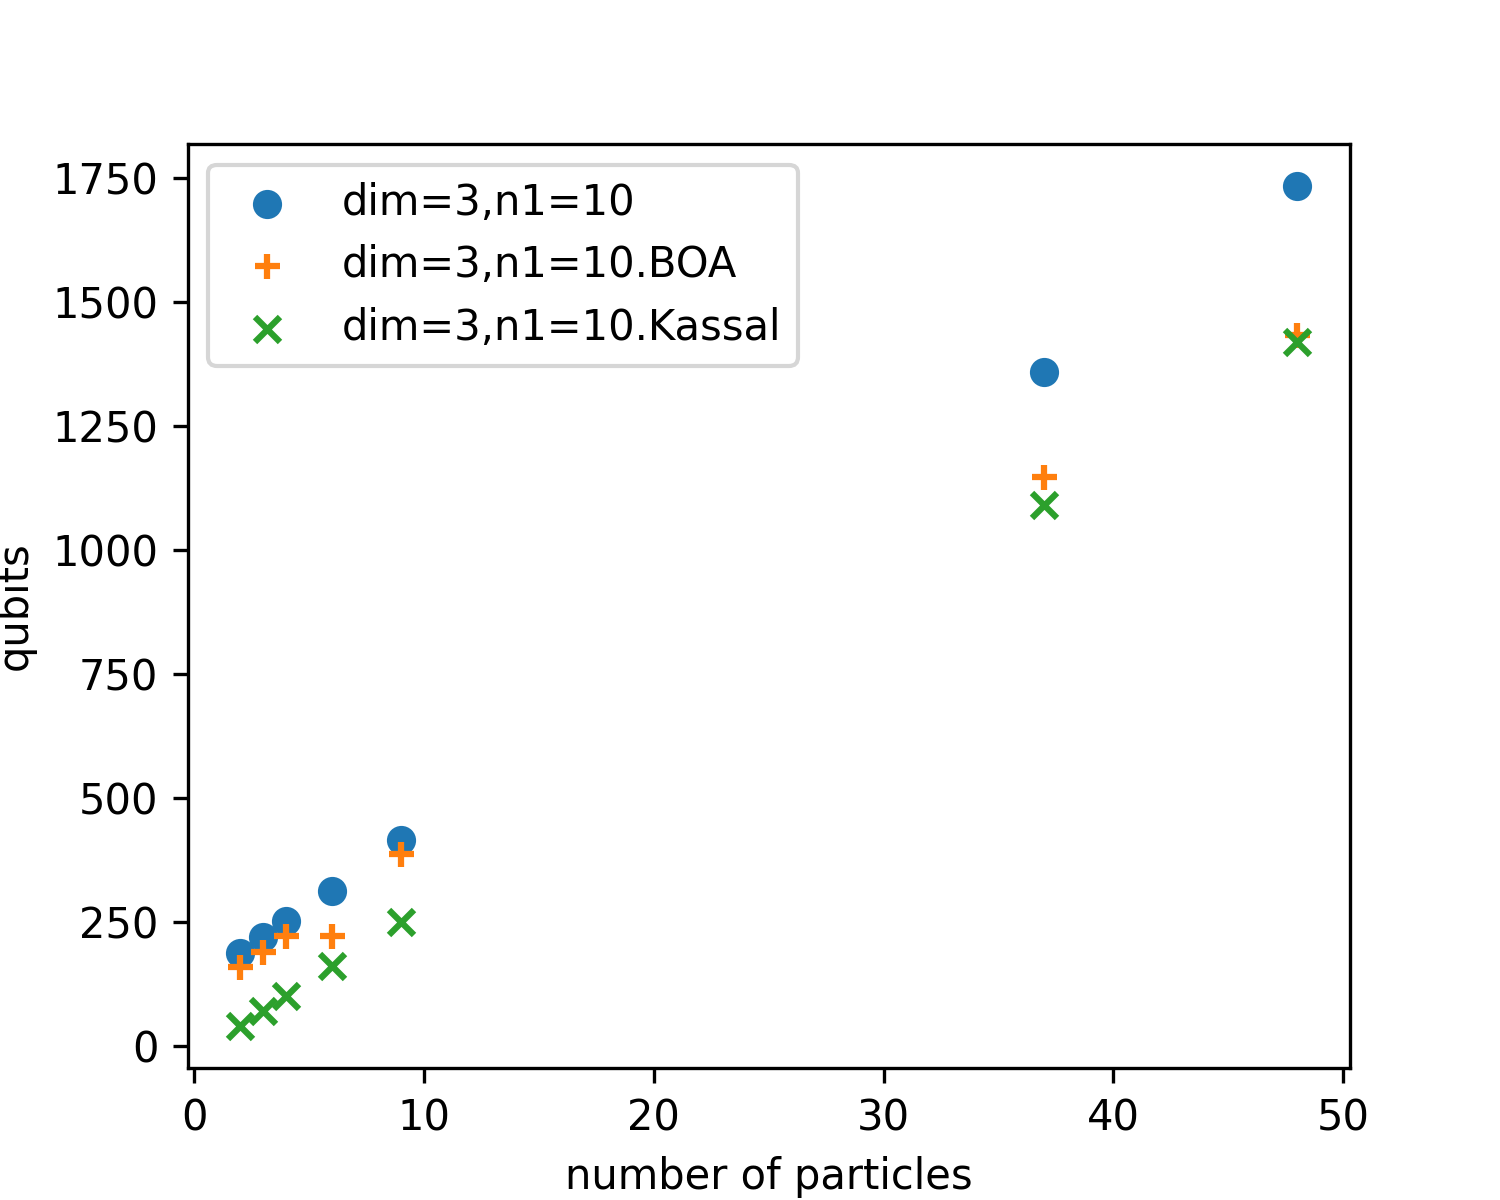
\includegraphics[width=0.6\textwidth]{paper2025_figs/circuit-size-qubits.png}
    \caption{粒子数とqubit数の関係}
    \label{fig:qubit-for-some-molecules}
    \begin{flushleft}\small

        粒子数の異なるいくつかの分子に対して、qubit数の関係を示している。粒子数
        (number of particles)は電子数と原子数の和である。各点が表している原子な
        いし分子は、粒子数の順に \ce{H}, \ce{He}, \ce{Li}, \ce{H + H2}, \ce{O},
        glycine(\ce{C2H5NO2}), Alanine(\ce{C3H7NO2}) である。 「\verb|+|」の点
        は原子核位置を固定の条件による値である(Born-Oppenheimer近似:BOA)。
        「\verb|x|」の点はKassal\cite{kassal2008.pnas.0808245105}に掲載の式に
        よる値である。
    \end{flushleft}
\end{figure}

いくつかの原子ないし分子に対して本回路生成プログラムでシミュレータの回路を生成さ
せた時の粒子数とqubit数の関係を図\ref{fig:qubit-for-some-molecules}に示す。この
図はエミュレータでの実行は無視してqubit数を制約なく使っている。座標のqubit数は10
ビットとしており、3次元のモデルとして計算している。演算は算術演算ゲートを用いて
いる。粒子数に線形なqubit数が必要であることが分かる。
\clearpage


\section{クーロンポテンシャルの極の扱い}
\label{sec:coulomb-potential-handling}
本研究では原子モデルを扱うためクーロンポテンシャルを量子回路によって計算する。原
子モデルに対するハミルトニアンシミュレーションではクーロンポテンシャルの極の扱い
方を定める必要がある。時間発展計算においてはポテンシャル$-1/r$と波動関数$\psi$の
積が各格子点の座標で計算される。この積をポテンシャルの極で計算すると発散してしま
う。これに対処する方法は大きく2つに分類される。(a)粒子間距離が０でも発散を起こさ
ないようなポテンシャルの近似式を導入する方法と、(b)原子核と電子の座標の離散化の
定義を変えることで計算上では両者の距離がゼロになることを防ぐ方法である。 (a)の近
似式の例を2つ検討する。一つ目の近似式(a1)は、極を含む格子でのポテンシャルエネル
ギーの平均値をその格子での代表値として用いる方法である。二つ目の近似式(a2)は、粒
子間距離を求めるノルム計算にオフセット項を加えたポテンシャル関数であり、soft
core ポテンシャルと呼ばれる。この関数はハミルトニアンシミュレーションにおいて
クーロン項計算の発散を防ぐ手段としても検討されている
\cite{Childs2022quantumsimulationof,Kivlichan_2017}。また、電子の運動方向が拘束
されている物理系のモデルとしても分析されている\cite{Hall2009.PhysRevA.80.032507,
Fernandez_1991, LiChen2021.doi:10.1021/acs.jpca.1c00698}。

(b)の原子核と電子の座標の離散化の定義を変える方法の例としては、
電子の位置は格子の中心になるものと定義しておく一方で、原子核の座標はここから格子
の刻みの1/2だけいずれかの軸方向にずらした位置として定義する方法が提案されている
\cite{Chan2023.sciadv.abo7484}。この方法ではポテンシャルの極の近傍でTrotter誤差
が大きくなるため、Chanらは計算結果を後付けの演算処理で補正している。本研究では
(b)の手法は取り上げない。

時間発展演算子のポテンシャルエネルギー項の回路 $\Thetaep$ ではクーロンポテンシャ
ルと波動関数の値の積が計算される。波動関数の値がポテンシャルの極においてゼロでは
ない場合、この計算は問題となる。本報告で扱う波動関数の中でこれに該当するのは、2
次元モデルの波動関数のうち方位量子数$m=0$ である$\Psi_{0,0}^{\mathrm{2D}}$と
$\Psi_{1,0}^{\mathrm{2D}}$ の二つの解である。

\subsection{極を含む格子の代表値を用いる近似式}
(a1)の近似式は、極の座標以外では本来の式を用い、極においては有限の値
$-1/\Delta_1$を返す式として次のように定義する。
\begin{equation}
\HaOne(r) = \begin{cases}
-\frac{1}{r} & (r>0) \\
-\frac{1}{\Delta_1} & (r=0)
\end{cases}\label{eq:Ha1r}
\end{equation}
$\HaOne$は、回路としての実装コストを抑えることができる式である。本研究で実装した
固定小数点の除算回路では、ゼロによる除算を行うと表現可能な最大値、すなわち全ビッ
トが1の値が得られる。その時の値がここでの$1/\Delta_1$の値としてそのまま使えるの
であれば回路として追加の要素が不要になる。ポテンシャル計算のためには除算は整数部
$1$桁、小数部$\nb$桁の固定小数点で行っている。全ビットが1の値は2進数で1が$\nb+1$
桁続いた値 $(2^{\nb+1}-1)\times2^{-\nb}=1.11\ldots1_2\simeq2_{10}$である。これは
$r=0$の時に$1/r$の演算結果が約2になることを意味している。$r$の単位が$\deltar$で
あると考慮するとこれは$r=\deltar/2$の時の計算結果に相当する。これは
$\Delta_1=\deltar/2$に取ることに該当する。

まず、$\HaOne$において $\Delta_1$ を選ぶ方法について述べる。ここでは波動関数が既
知である場合の式の導出を示す。

1次元モデルの $\PsiOneD_1$ においてはポテンシャルの極での波動関数の値がゼロであ
り、ポテンシャルの値は有限であればよいため、近似式としては追加の回路が不要にな
る、$\Delta_1=\deltar/2$を用いるものとする。

2次元モデルにおいては、方位量子数$m$の値に応じて、ポテンシャルの極における波動関
数の値がゼロである場合と非ゼロである場合とがある。$m\ne0$の解ではゼロにな
り、$m=0$では非ゼロになる。非ゼロの関数の例として$\PsiTwoD_{0,0}$ と
$\PsiTwoD_{1,0}$を取り上げて、$r=0$におけるポテンシャル関数の適切な値を検討す
る。$m=0$の場合は代表値は任意の値でよいので、$m=1$の場合に対して求めた$\Delta_1$
の値を、$m=0$の場合にも適用することができる。

近似式 $\HaOne$ におけるパラメータ $\Delta_1$ は、次のように定めることができる。
クーロンポテンシャル項の計算では、各グリッドの中心座標におけるポテンシャルの値を
代表値として用いて、それにグリッドの面積を掛けることで積分値を近似する。極と重な
る格子点ではこの代表値が発散してしまうが、格子の領域内で積の平均値を求める積分計
算は２次元以上のモデルであれば発散しない。そこで、積分値と同じ値が得られるような
代表値でもって、極におけるポテンシャルの近似値に定めることを考える。

極を中心としたグリッドの内接円を考え、その円内のクーロンポテンシャルの代表値が
$-1/\Delta_1$ であるとした時のエネルギーの値 $W_{n,m}^\prime$ を計算する。次に、
同じ領域に対して真のクーロンポテンシャルを用いて計算したエネルギーの値 $W_{n,m}$
を計算する。その後、両者が一致するように $\Delta_1$ の値を求める。これを
$(n,m)=(0,0)$と$(1,0)$ のそれぞれに対して求める。$W_{n,m}$と$W_{n,m}^\prime$はそ
れぞれ、
\begin{align}
    W_{n,m}&=\int_{\theta=0}^{2\pi}d\theta\int_{r=0}^{\deltar/2}
    \Hep(r)\abs{\PsiTwoD_{n,m}(r)}^2r dr\\
    W_{n,m}^\prime&=\pi\left(\frac{\deltar}{2}\right)^2
    \HaOne(0)\PsiTwoD_{n,m}(0) \notag \\
    &=-\frac{\pi\deltar^2}{4\Delta_{1,n,m}}
    \sqrt{\frac{q_0^3(n-\abs{m})!}{\pi(n+\abs{m})!}}
    L_{n-\abs{m}}^{2\abs{m}}(0)
\end{align}
である。$(n,m)=(0,0)$と$(1,0)$に対してそれぞれ$W_{n,m}=W_{n,m}^\prime$ を解くと、
\begin{align}
    \Delta_{1,0,0} &=\frac{q_0\deltar^2}{4(-e^{-q_0\deltar}+1)}
    \simeq \frac{q_0\deltar^2}{4(-1+q_0\deltar+1)}=\frac{\deltar}{4}
    \label{eq:delta-1-0-0}\\
    \Delta_{1,1,0} &=\frac{q_0\deltar^2}{4((-1+q_0^2\deltar^2)e^{-q_0\deltar}+1)}
    \simeq \frac{q_0\deltar^2}{4((-1+q_0^2\deltar^2)(1-q_0\deltar)+1)}
    \simeq\frac{\deltar}{4}
    \label{eq:delta-1-1-0}
\end{align}
が得られる。近似はいずれも$\deltar\ll1$ である場合のものである。導出は付録
\ref{chap:appendix_derivation_derivation}に示す。

$\HaOne (r)$おける $\Delta_1$の値を空間離散化の刻み $\deltar$と大きさの逆数$a$を
用いて $1/a=\deltar/\Delta_1$ と表し $1\le a\le 8$の範囲でのエネルギー計算値を複
数種類の$\nb$に対して求めたグラフを図\ref{fig:Ha1-vs-delta1}に示す。
このグラフの計算値はシミュレータ回路による演算が不能な範囲の条件を含む
ため、量子回路ではなく等価な演算をする古典プログラムにより計算した。
図\ref{subfig:Ha1-energy-0-0}と\ref{subfig:Ha1-energy-1-0}を見ると２種類の波動関数
$\PsiTwoD_{0,0}$と$\PsiTwoD_{1,0}$ のそれぞれにおいて、$a=4$ すなわち
$\Delta_1=\deltar/4$ の時にエネルギー固有値の解析解にほぼ一致する結果が得られ
た。いずれのグラフも$a=4$を境に誤差の符号が反転している。 $\Delta_1$の値を導出し
た式(15)では、$\deltar\ll1$の時の近似値が$\deltar/4$であるが、グラフを見ると
$\deltar/4$から外れると誤差が生じるので最適条件が各ビット数で共通になっている。

\begin{figure}[ht]
    \centering
    \begin{subfigure}{0.45\columnwidth}
        \centering
        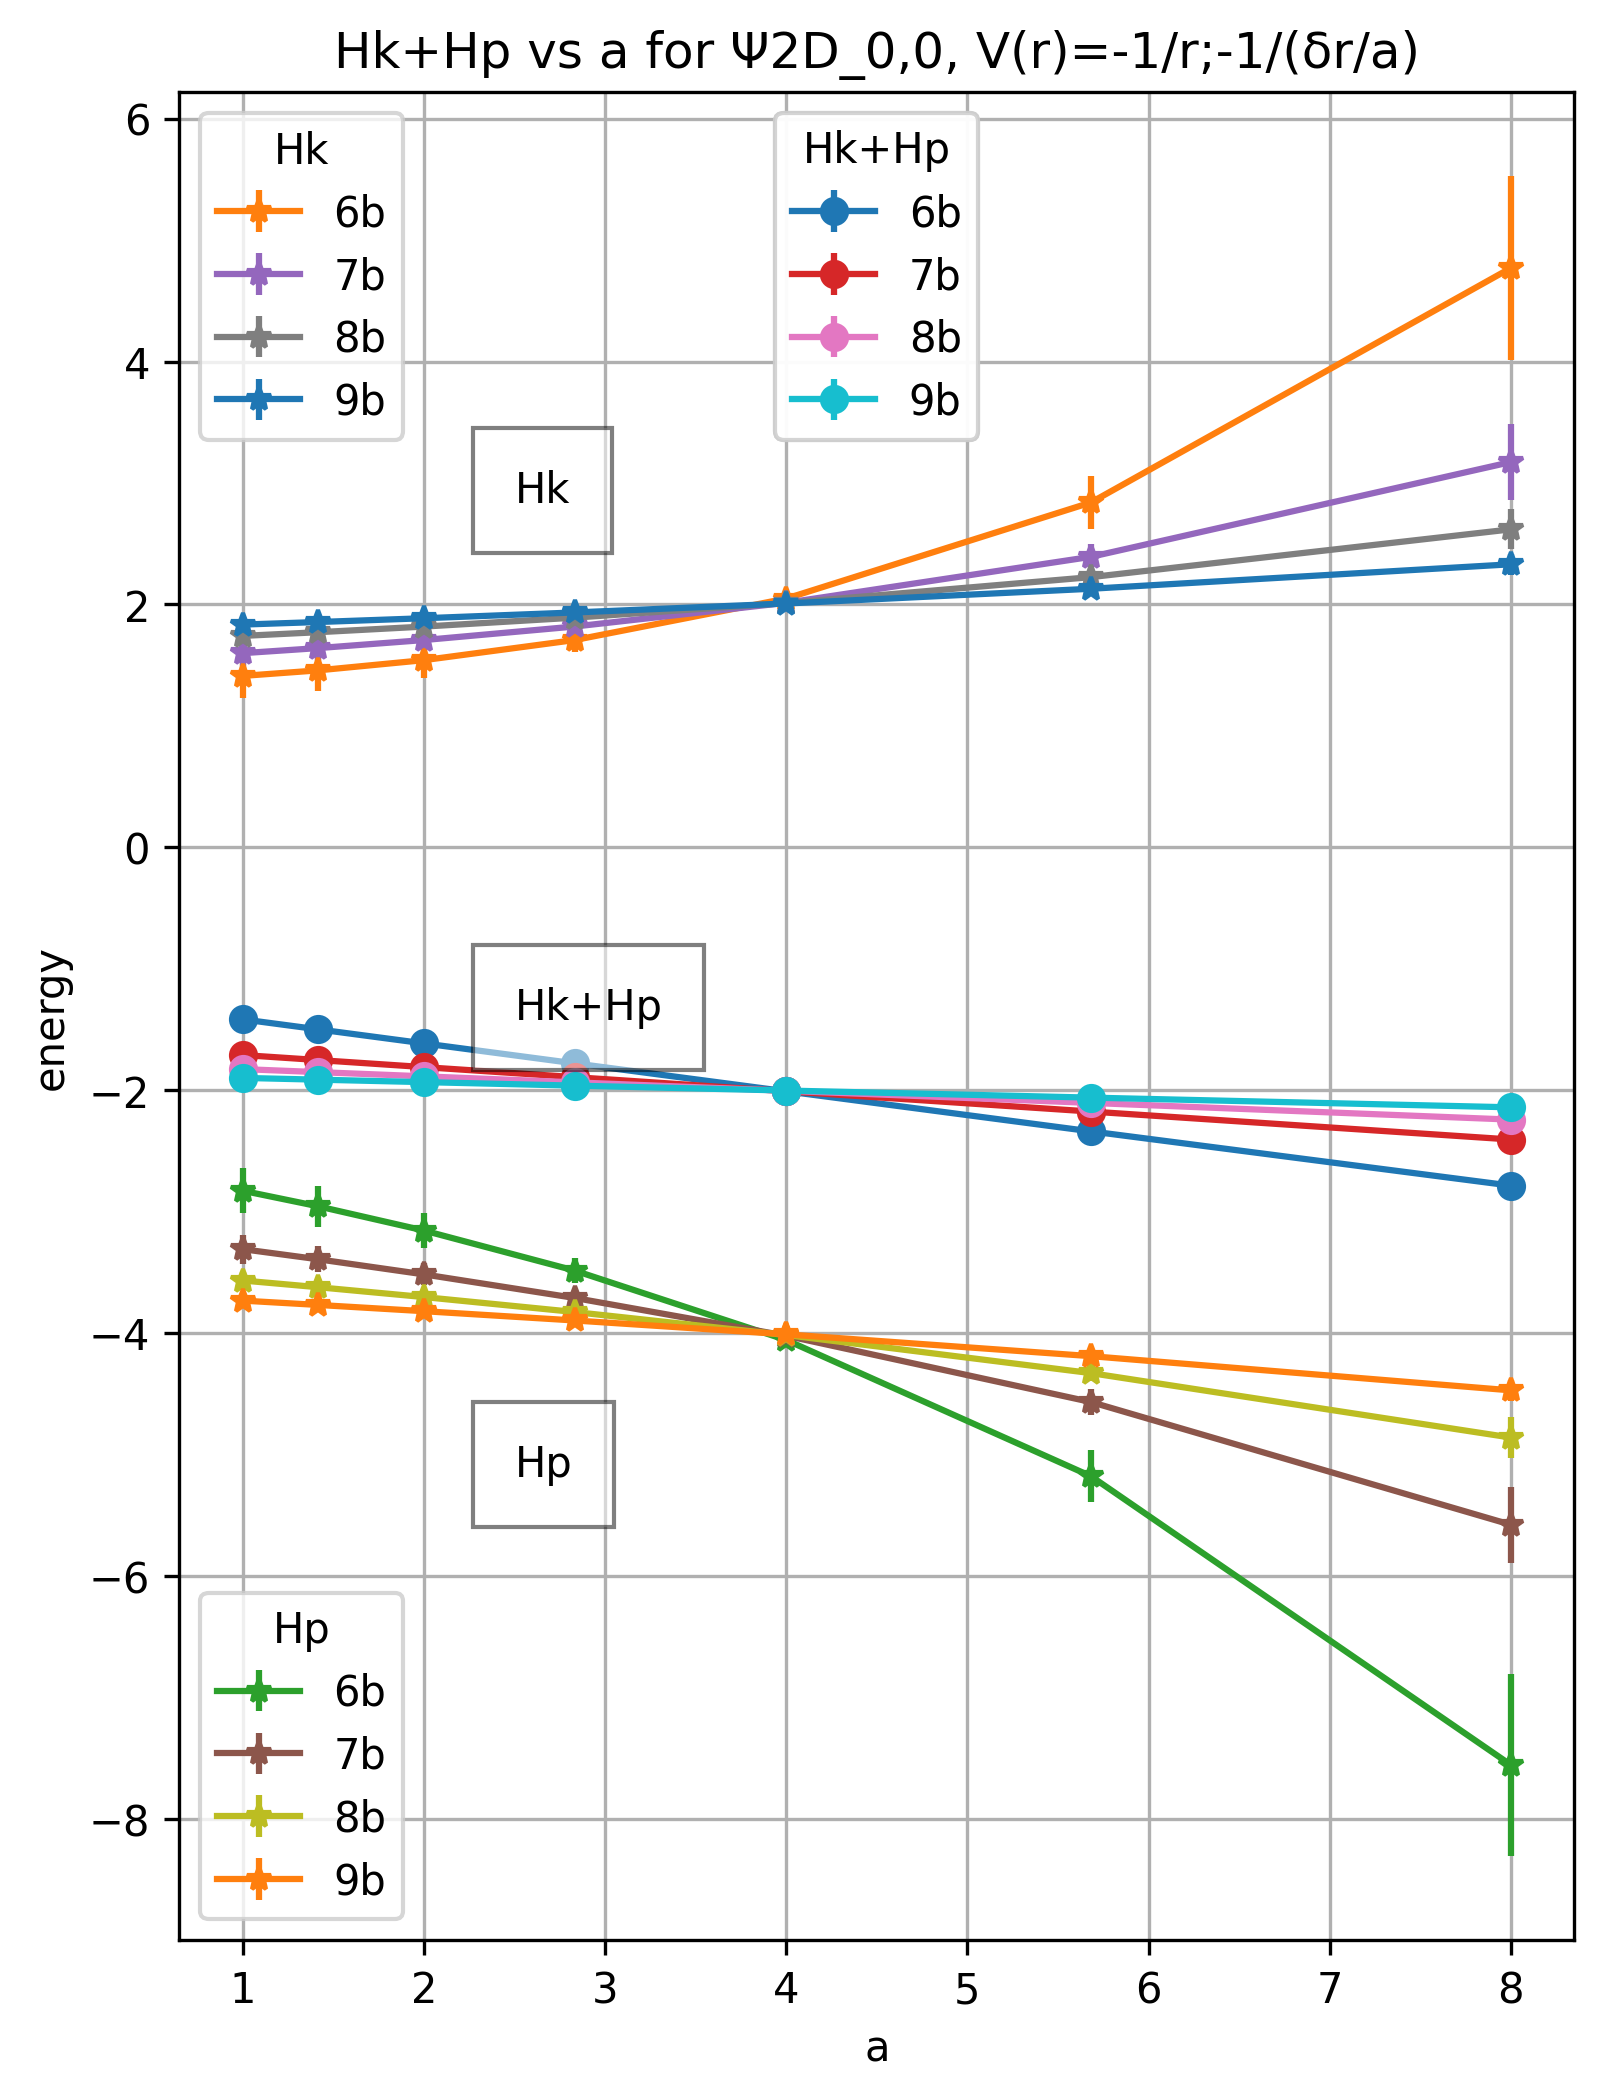
\includegraphics[width=1\columnwidth]{paper2025_figs/compare_energy/compare_energy_h2D_TO2_r0lim_0_0.png}
        \caption{$\PsiTwoD_{0,0}$}
        \label{subfig:Ha1-energy-0-0}
    \end{subfigure}
    \begin{subfigure}{0.47\columnwidth}
        \centering
        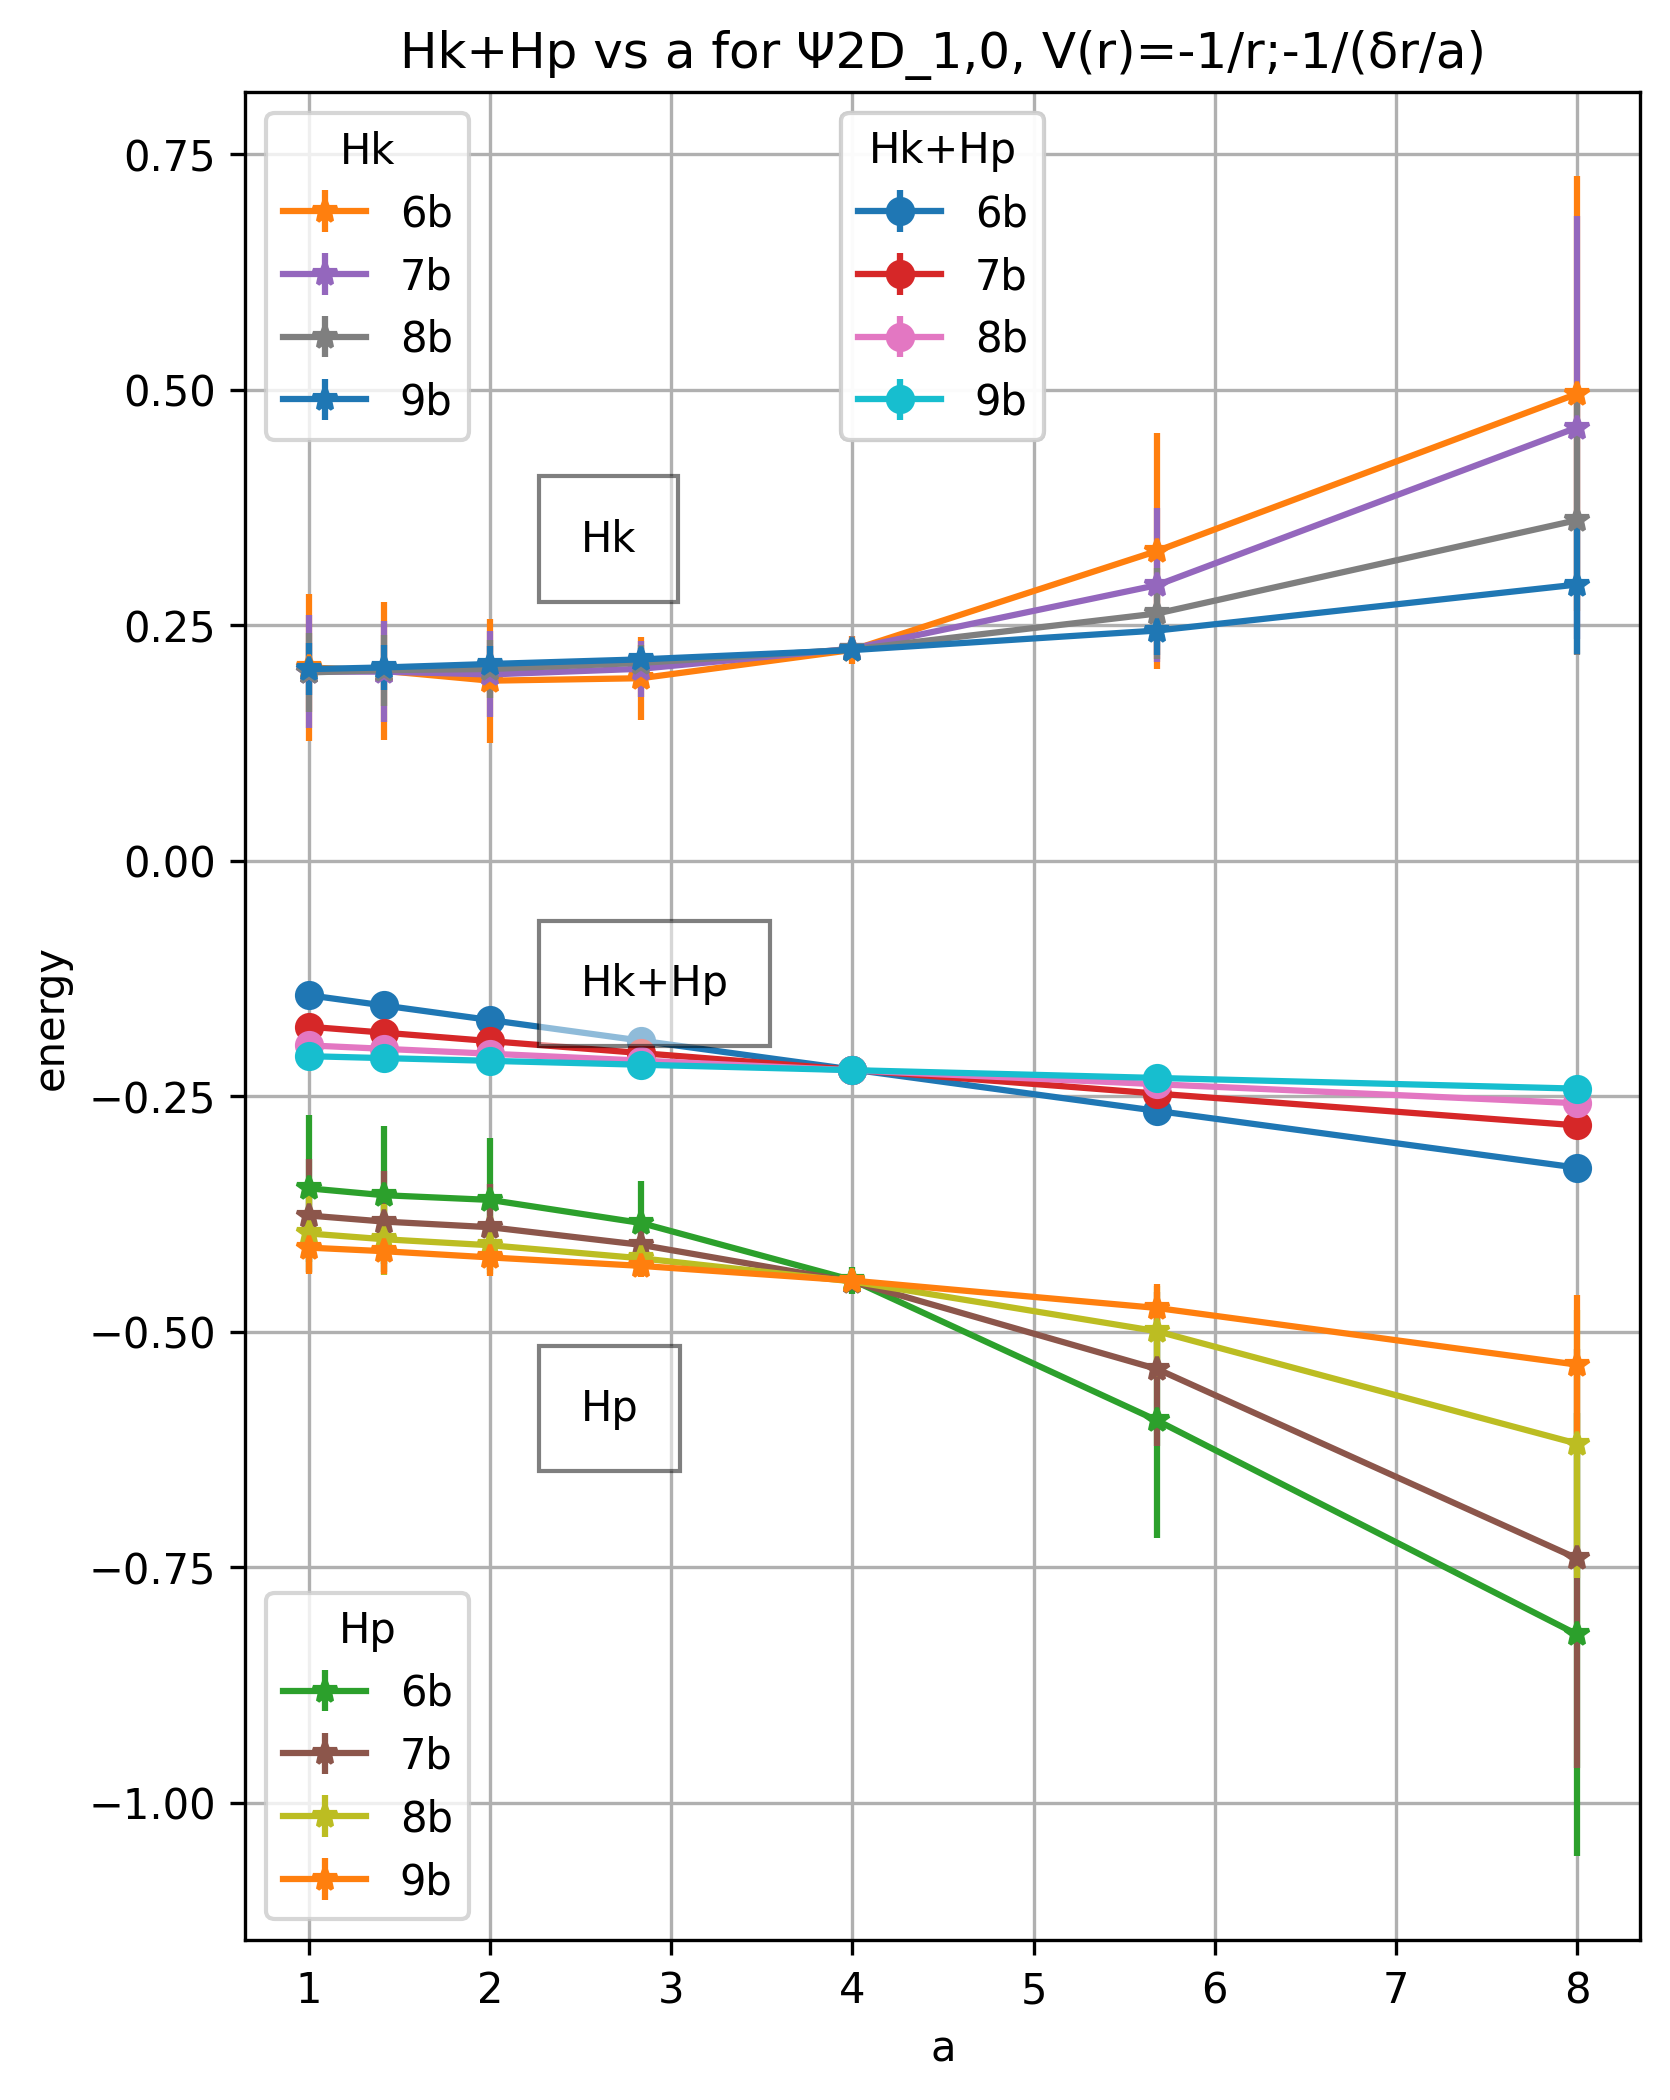
\includegraphics[width=1\columnwidth]{paper2025_figs/compare_energy/compare_energy_h2D_TO2_r0lim_1_0.png}
        \caption{$\PsiTwoD_{1,0}$}
        \label{subfig:Ha1-energy-1-0}
    \end{subfigure}
    \caption{近似式$\HaOne(r)$において$\Delta_1$の値を変えた時のエネルギー値の変化}
    \label{fig:Ha1-vs-delta1}
    \begin{flushleft}\small
        (a) $\PsiTwoD_{0,0}$に関して $\Delta_1=\deltar/a$とおいて $a$ を変化させ
        たグラフ。$a$ の値は比が$\sqrt{2}$ の等比級数としている。各ビット数共に
        $a=4$ の時すなわち $\Delta_1=\deltar/4$ の時に$\Hk+\Hp$ が解析解のエネル
        ギー固有値の $-2.0$ に近い値を示している。(b)$\PsiTwoD_{1,0}$の時のグラ
        フ。ここでも $a=4$ においてエネルギー固有値の $-0.2222$ に近い値を示して
        いる。
    \end{flushleft}
\end{figure}

\clearpage
\subsection{soft-core ポテンシャルによる近似式}
(a2)の近似式は、距離を求めるノルム計算にオフセット項を加えた、soft-core
ポテンシャルの式であり、次のように定義する\cite{Kivlichan_2017}。
\begin{equation}
\HaTwo(r) = -\frac{1}{\sqrt{r^2+\Delta_2^2}}\label{eq:Ha2r}
\end{equation}

$\HaTwo(r)$ について、式の中での定数$\Delta_2$ を変化させた時のエネルギー計算値
を図\ref{fig:Ha2-vs-delta2}示す。なお、これらのグラフの計算値はシミュレータ回路ではな
く古典プログラムにより計算した。

$r=0$においては$\HaTwo(0)=-1/\Delta_2$となり、$\HaOne(r)$と同じ式となる。その結
果、$\HaOne(r)$の時と同じ$\Delta_2=\deltar/4$を用いた時にエネルギー固有値の解析
解に近い値が得られている。$r\ne0$においては両者には差があるが、エネルギー計算値
には大きな差は見られない。図 8に示すグラフを見ると、$\HaTwo(r)$においても
$\Delta_2=\deltar/4$の時にエネルギー固有値の解析解に近い値が得られている。

\begin{figure}[ht]
    \centering
    \begin{subfigure}{0.45\columnwidth}
        \centering
        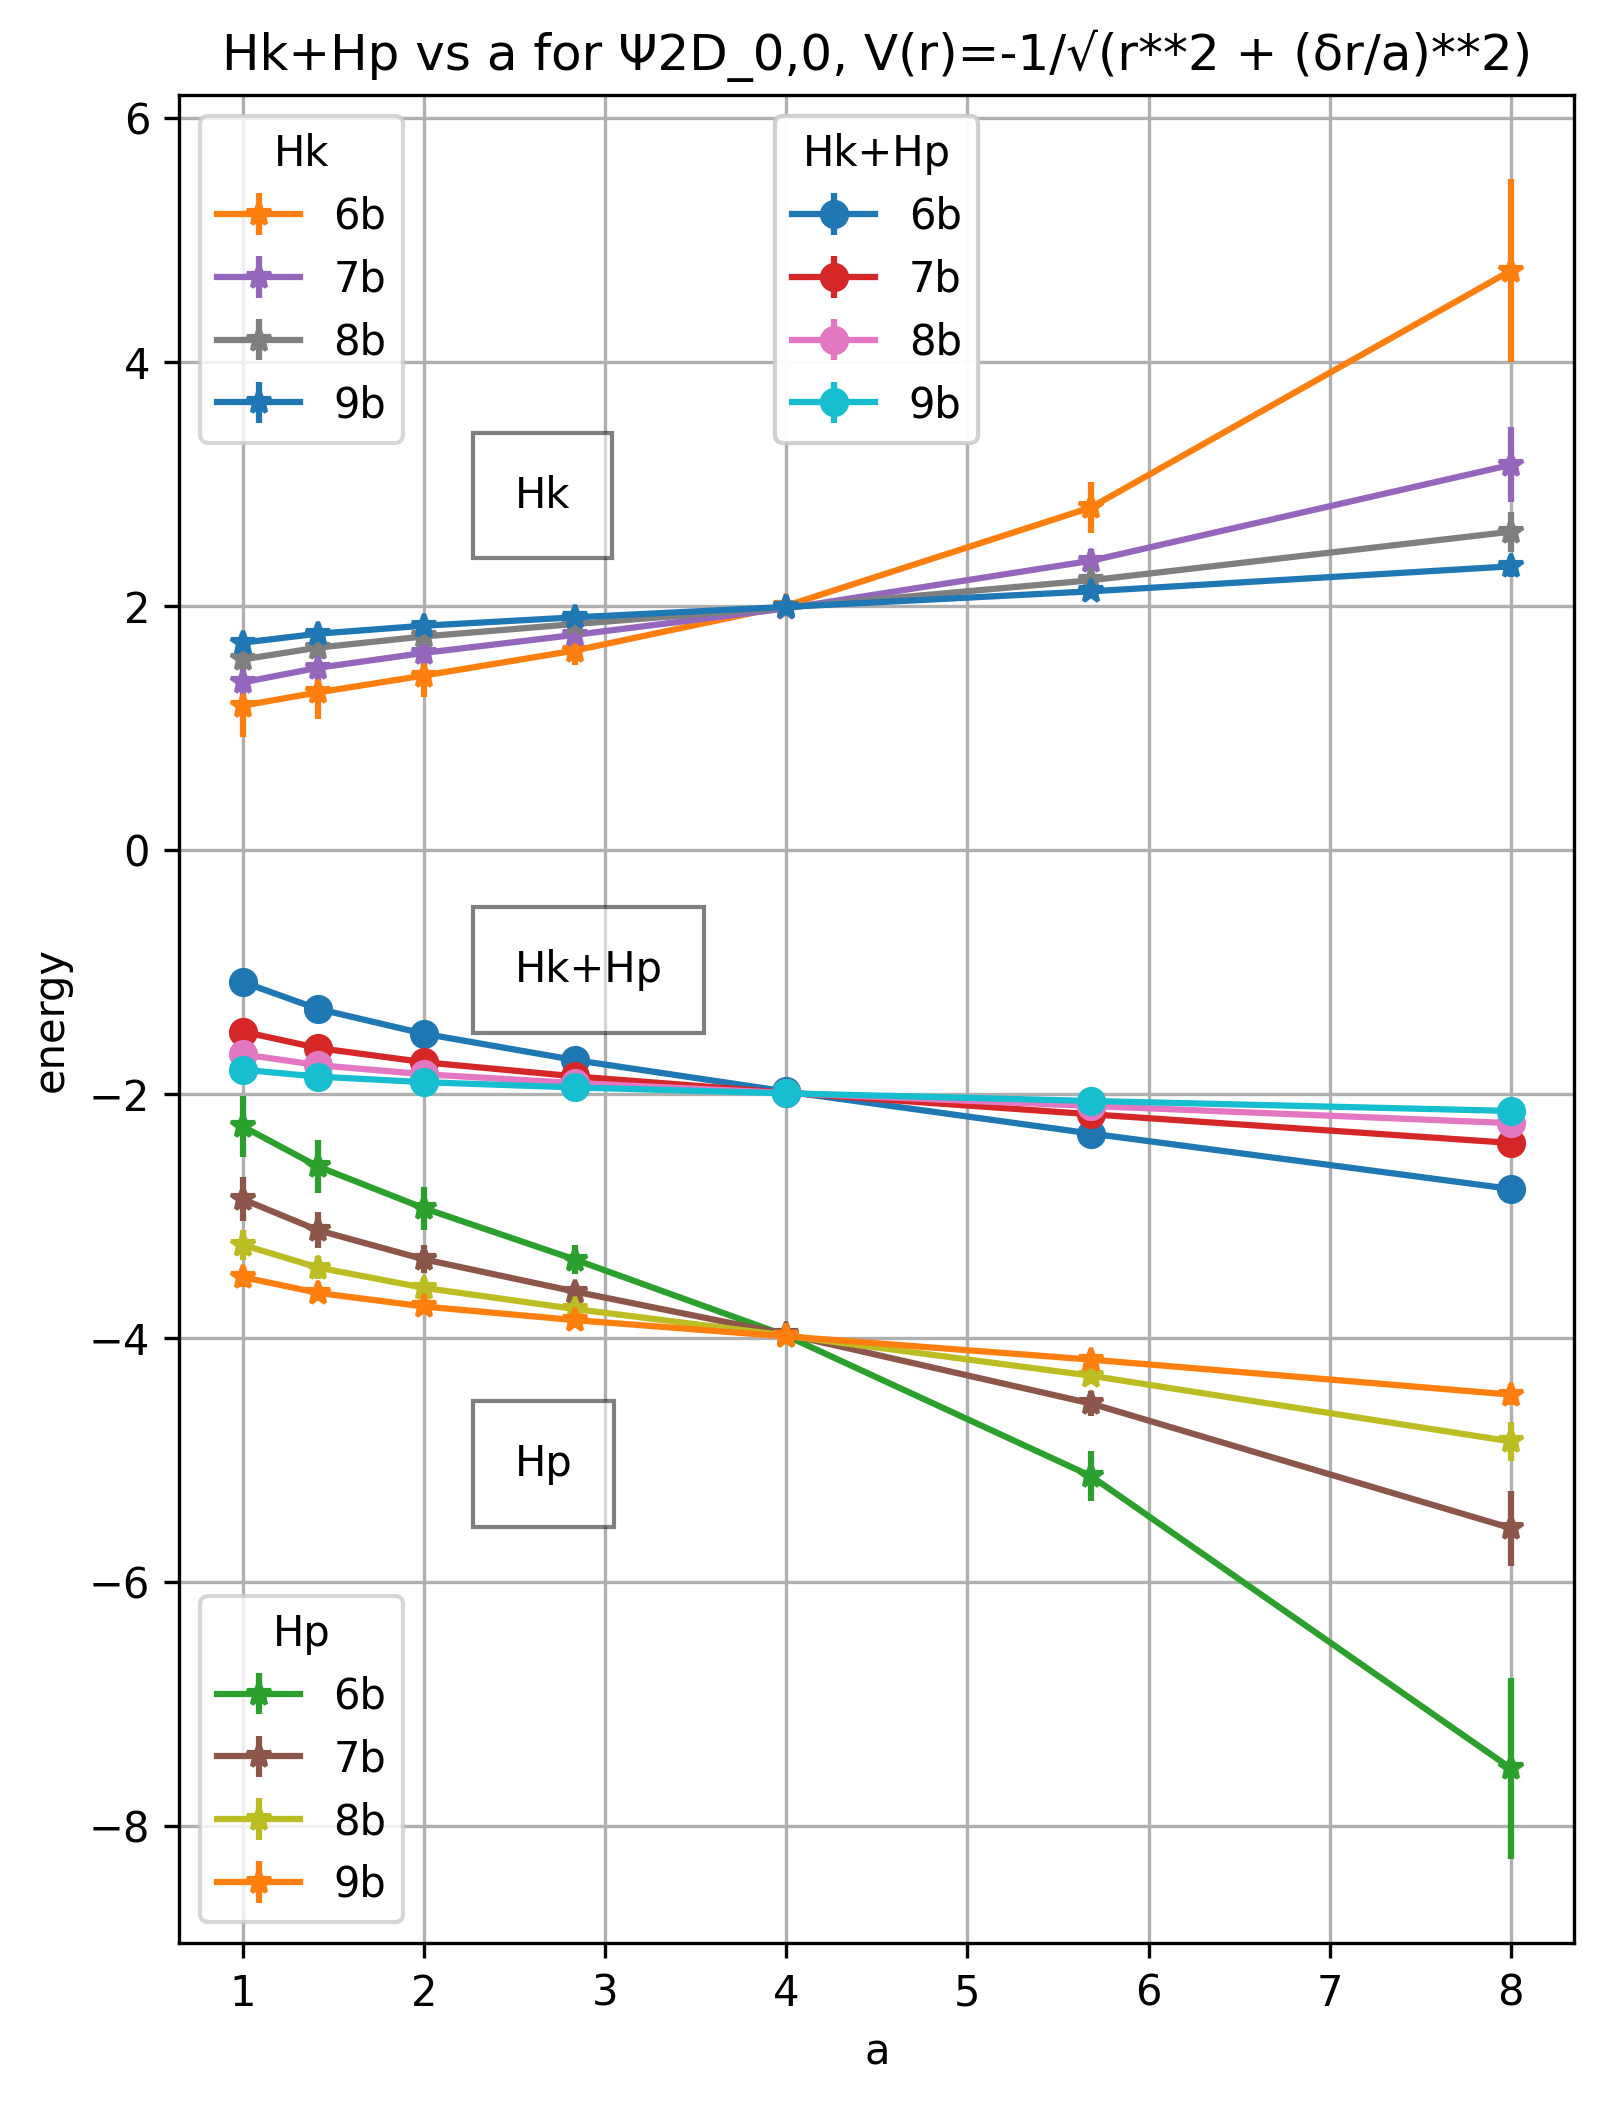
\includegraphics[width=1\columnwidth]{paper2025_figs/compare_energy/compare_energy_h2D_TO2_rofs_0_0.png}
        \caption{$\PsiTwoD_{0,0}$}
        \label{subfig:Ha2-energy-0-0}
    \end{subfigure}
    \begin{subfigure}{0.47\columnwidth}
        \centering
        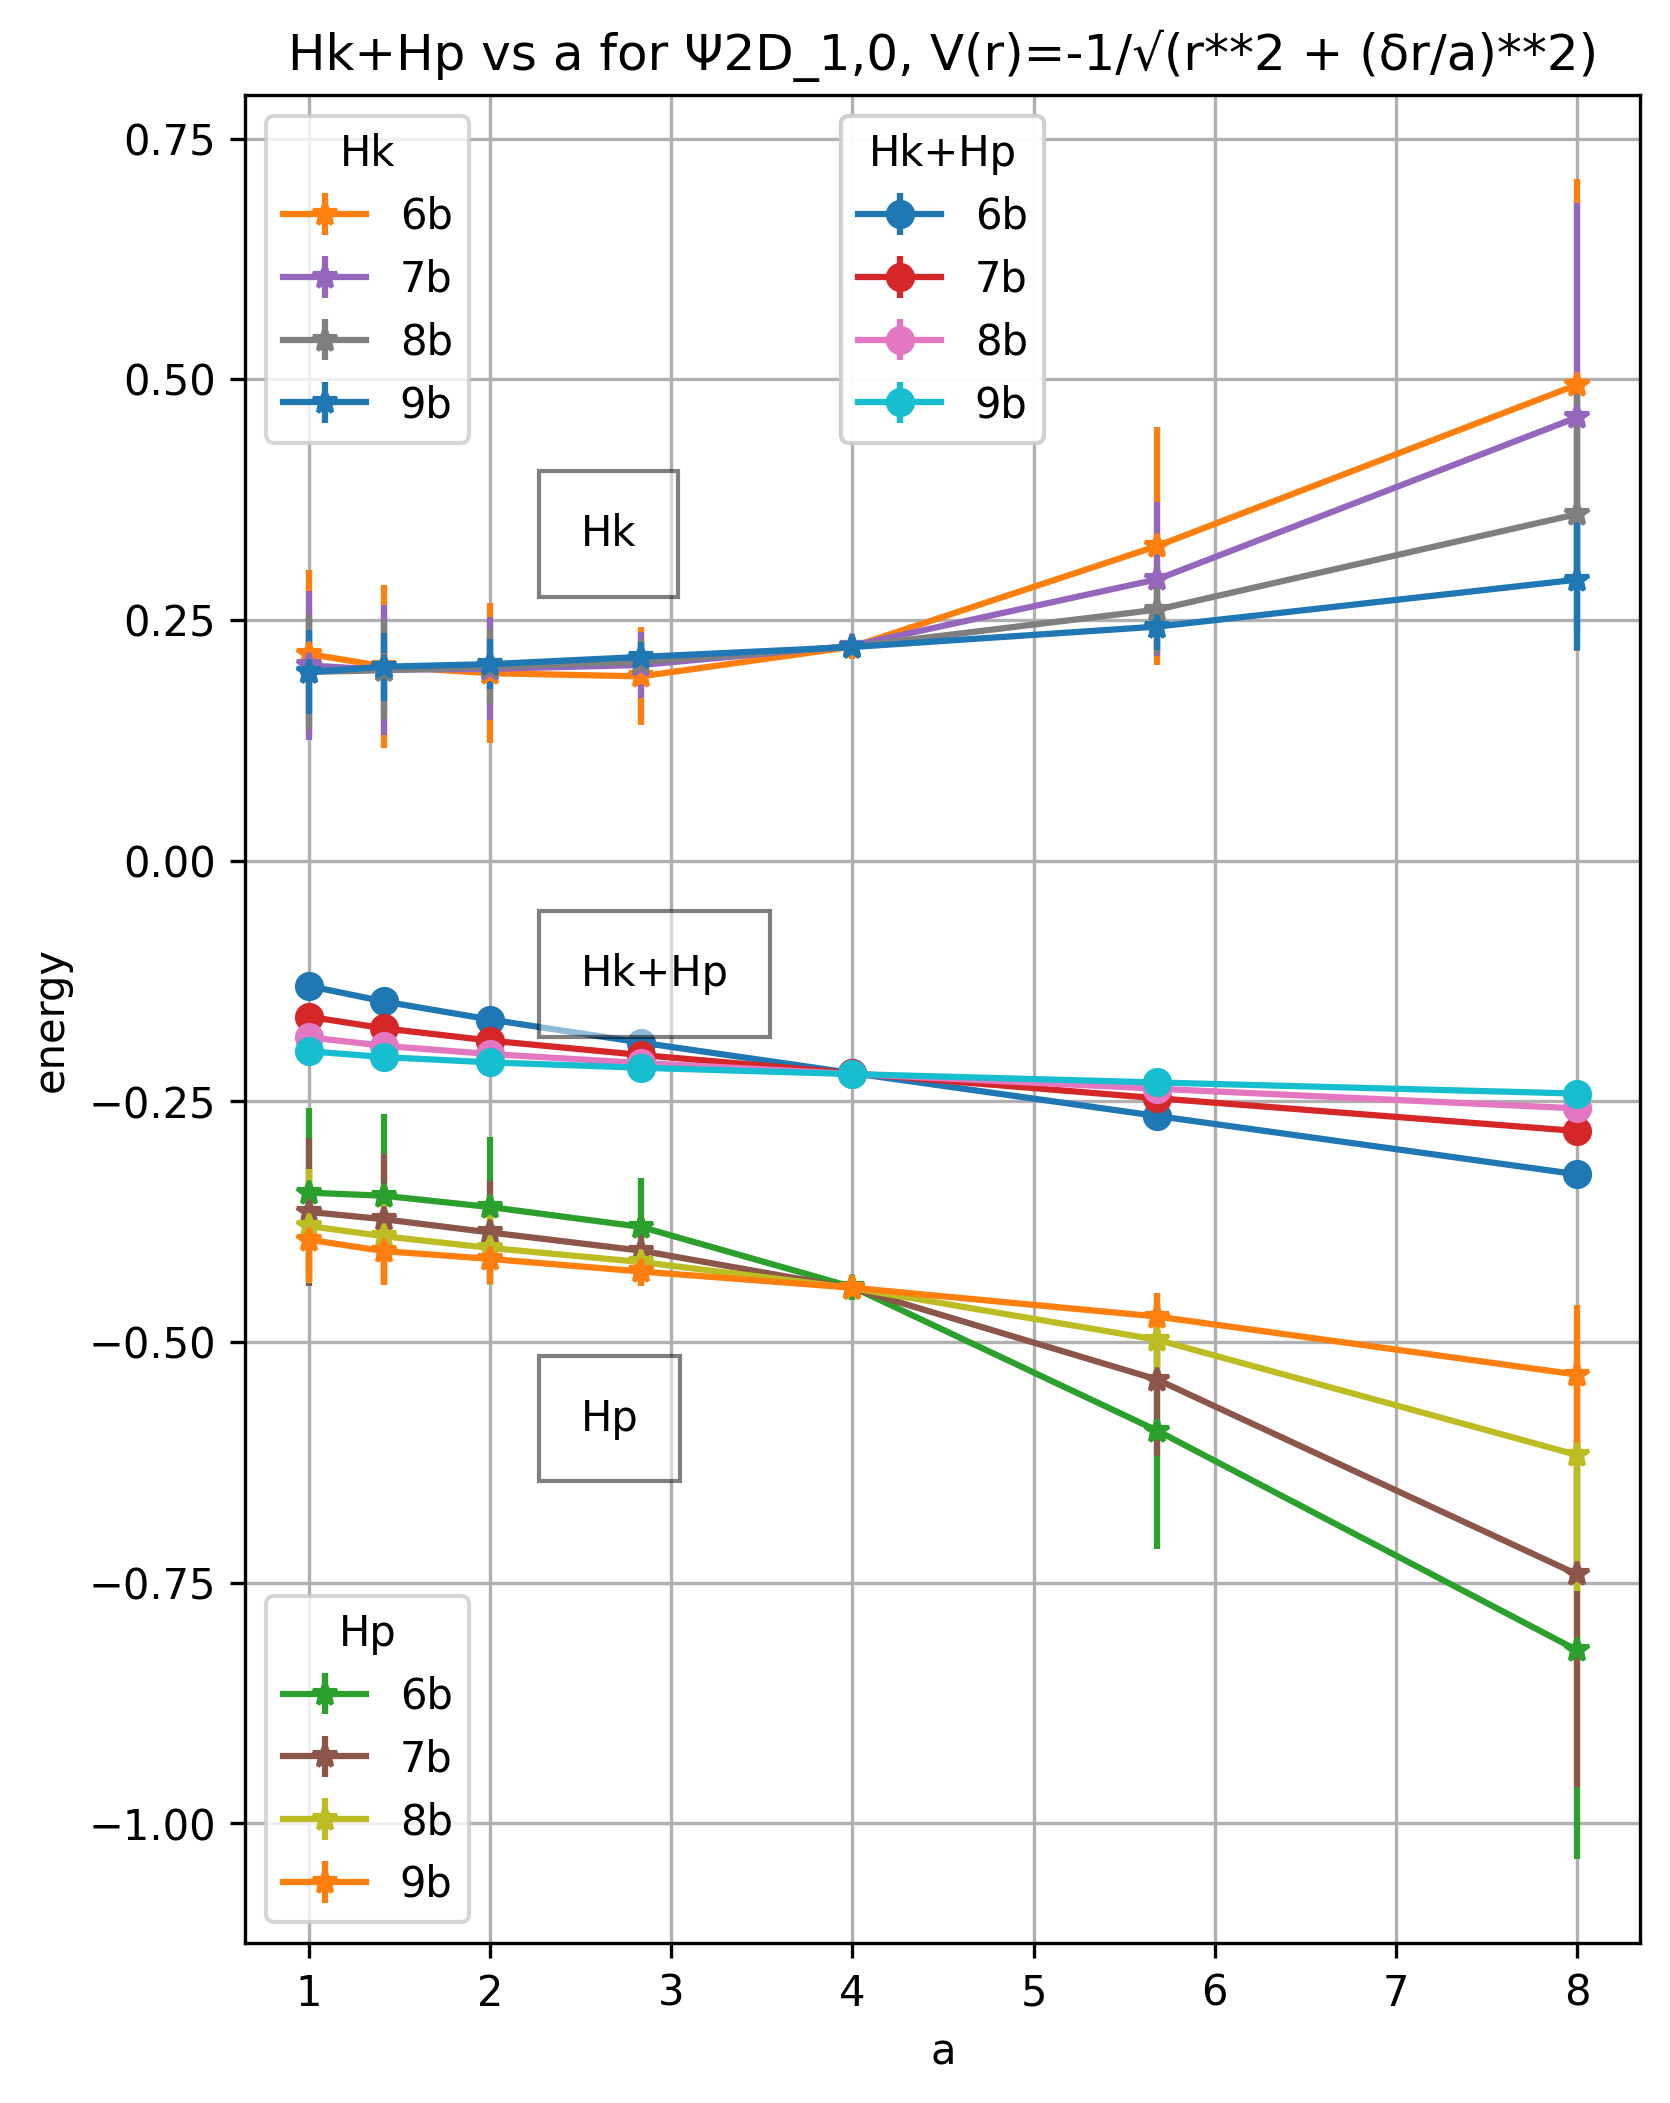
\includegraphics[width=1\columnwidth]{paper2025_figs/compare_energy/compare_energy_h2D_TO2_rofs_1_0.png}
        \caption{$\PsiTwoD_{1,0}$}
        \label{subfig:Ha2-energy-1-0}
    \end{subfigure}
    \caption{近似式$\HaTwo(r)$において$\Delta_2$の値を変えた時のエネルギー値の変化}
    \label{fig:Ha2-vs-delta2}
    \begin{flushleft}\small

        (a) $\PsiTwoD_{0,0}$に関して $\Delta_2=\deltar/a$とおいて $a$ を変化させ
        たグラフ。$a$ の値は比が$\sqrt{2}$ の等比級数としている。各ビット数共に
        $a=4$ の時すなわち $\Delta_2=\deltar/4$ の時に$\Hk+\Hp$ が解析解のエネル
        ギー固有値の $-2.0$ に近い値を示している。(b)$\PsiTwoD_{1,0}$の時のグラ
        フ。ここでも $a=4$ においてエネルギー固有値の $-0.2222$ に近い値を示して
        いる。

    \end{flushleft}
\end{figure}

\clearpage

\section{誤差を最小にするシミュレーションパラメタの決定}
\label{sec:parameter-selection-for-minimum-error}
ハミルトニアンシミュレーションを行うにはいくつかのシミュレーションパラメータの設
定が必要になる。計算誤差を所望の範囲に収めるために必要となるシミュレーションの空
間分解能やステップ時間の検討は多くされており、所望の精度を得るために必要となる
qubit数の算出が検討されている\cite{FEIT1982412, Kivlichan_2017,
Chan2023.sciadv.abo7484}。 本報告では既存の検討とは逆に、qubit数が所与の場合にシ
ミュレーションパラメータに課される制約条件やトレードオフ関係に着目して最良な精度
をもたらすパラメータの決定方法を示す方法を検討する。本報告では時間発展にTrotter
分解を用いるが、グリッド法で定義されたモデルにTrotter分解で時間発展させた場合に
計算結果として得られる波動関数には、以下の誤差が含まれる。

\begin{equation}
\errtotal \leq \errspatial + \errtemporal
\label{eq:error-total-decomposition}
\end{equation}

ここで $\errtotal$ は誤差の合計、$\errspatial$ は空間離散化のパラメータに起因す
る誤差、$\errtemporal$ は時間離散化のパラメータに起因する誤差である。両者はさら
に要素に分解される。それぞれの要素ごとに特性が知られているが、特定の要素だけ改善
しても他の要素の成分が優勢の場合には全体としての改善が得られない。そこで、トレー
ドオフ関係を考慮しながら支配的な誤差項を削減していくことが必要になる。

トレードオフとして本報告で考察するのは空間座標の刻み$\deltar$と、シミュレーショ
ン対象直方体の１辺の長さ$L$の関係である。グリッド法では計算対象の直方体空間を定
めてその領域に収まる範囲の波動関数を計算する。領域外では波動関数の振幅が無視され
るので、得たい精度に照らして領域の境界での波動関数の振幅が無視できる大きさとなる
ように十分大きな寸法に設定することが必要である。領域の一辺の長さ$L$が所望の精度
に照らして十分であるかどうか判断する方法として、シミュレーション対象の波動関数か
ら領域境界面上の電子密度の最大値を数値的に算出し、それが目標値$\rho_0$以下となる
ように$L$を定める方法が提案されている\cite[Supplementary material, S8, A. Space
Cost]{Chan2023.sciadv.abo7484}。$L$を拡大するにはqubitの数を増やすか、分解能を粗
くする必要がある。qubit数が多い計算環境下では必要に応じてqubit数を増やすことがで
きるが、qubit数が制限されている条件下では座標の量子化の刻み$\deltar$を大きくする
ほかない。この場合、空間の寸法と分解能がトレードオフ関係になる。このトレードオフ
を加味した寸法の決定方法については今まで具体的に論じられていない。本報告では波動
関数を仮定した上でこのトレードオフを数値的に評価し、適切なパラメータの値を決定す
る方法を示す。

時間刻み$\deltat$の満たすべき条件は２つあり、離散的フーリエ変換を用いることでサ
ンプリング定理からの要請に基づく条件\cite{FEIT1982412}とTrotter分解の誤差に起因
する条件である
\cite{Childs2021.PhysRevX.11.011020,Burgarth2024.PhysRevResearch.6.043155}。これ
らの両方を考慮する必要がある。

誤差を空間パラメータによる誤差と時間パラメータによる誤差に分かれると示した式
\ref{eq:error-total-decomposition}はさらに以下の要素に分けられる。
\begin{align}
    \errspatial &\equiv \errdisc + \errcutoff \\
    \errtemporal &\equiv \erralias + \errtrotter
\end{align}
ここで、$\errdisc$ は空間離散化による波動関数の近似誤差であり、$\errcutoff$ は計
算対象領域の直方体からはみ出た部分の波動関数の成分による誤差である。ま
た、$\erralias$ は有限の項数で波数表示されていることに伴うエイリアシング誤差であ
り、$\errtrotter$ はTrotter近似に起因する誤差である。

本節ではqubitの総数が所与の条件でこれらの誤差を小さくしていくためのパラメータの
決定方法を示す。空間パラメータによる２つの誤差 $\errdisc$ と $\errcutoff$ の対は
トレードオフ関係にあるので、トレードオフを考慮したパラメータ値 $\deltar$ の決定
方法を検討する。時間パラメータ $\deltat$ に関してはトレードオフが存在せず、サン
プリング定理から$\deltat$の上限値が、Trotter誤差の解析的評価からは予想される誤
差の上限が与えられるので、これらを考慮してパラメータを決定する。

\subsection{δrの決定方法}
\label{subsec:delta-r-selection-method}
本報告ではシミュレーション対象領域は周期境界条件を適用しており、空間の一辺の長さ
は各次元で共通で$L=2^{\nb}\deltar$ である。この空間の中央を座標系の原点とし、原点
に原子核を配置する。座標値が $[-L/2,L/2]$ からはみ出る部分に関しては波動関数がカッ
トオフされることになる。$\deltar$を小さくとると、$\errdisc$ が小さくなるという点
では好ましいが、$\deltar$に比例して$L$も小さくなるため、$\errcutoff$ は増大してしま
う。計算対象領域内の$\errdisc$と、$\errcutoff$ が拮抗する $\deltar$ を探すことで、二
種類の誤差の合計を最小にする $\deltar$ を求めることができる。

波動関数の二乗をシミュレーション領域上で積分した値$S_1$と領域外で積分した値$S_2$
をそれぞれ
\begin{align}
S_1 &= \int_{x,y,z=-L/2}^{L/2}\Psi(\bm{r})^{\ast}\Psi(\bm{r}) d\bm{r} \\
S_2 &= 1 - S_1
\end{align}
とする。

$S_1$に相当する離散化した座標での近似値を$S_d$とする:
\begin{equation}
S_d = \sum_{j}\abs{\Psi(\chij)}^2 \deltar^3
\end{equation}
このようにとると、
\begin{align}
\errdisc &\simeq \abs{S_1 - S_d} \label{eq:err-disc-definition}\\
\errcutoff &\simeq S_2 \label{eq:err-cutoff-definition}
\end{align}
となる。$\abs{S_d-S_1}+S_2$が最小となる$\deltar$が最適な$\deltar$の値である。

座標のqubit数 $\nb$ が一定の条件下で空間離散化のパラメータ $\deltar$ を変化さ
せるとグリッド数 $2^{(\nb)}$ は一定であるので $L=2^{(\nb)} \deltar$ が同時に増減
する。$\deltar$ が大きいと空間離散化誤差 $\errdisc$ が増大し $L$ が小さいとカット
オフ誤差 $\errcutoff$ が増大する。2つの誤差のトレードオフを考慮して $\deltar$ を
定める必要がある。

1次元のモデル $\psi_1^{1D}$ においていくつかの $\nb$ の値に関して空間離散化誤差
$\errdisc=|S_d-S_1|$ とカットオフ誤差 $\errcutoff=S_2$ を比較したグラフを
図 \ref{subfig:dq-tradeoff-1d} に示す。

グリッドの点が最も少ない $\nb=6$ の場合に着目すると、(A1)により、$S_2$の線と
$|S_d-S_1|$の線は$\deltar=0.22$ のあたりで交差する。(A2)においては$\nb=6$の線が
最小になる点に該当する。この値が2種類の誤差のトレードオフがバランスする値
である。$\deltar$と$L$ は比例しており(A3)からこの時 $L=14$ である。

qubit数が2つ多い $\nb=8$のケースに着目すると(A2)から、$\deltar=0.07\sim0.14$ の
範囲で値はほぼ0となっている。これは、この範囲で$\deltar$を変化させても、誤差の目
立った増減はないことを意味する。$\deltar<0.07$で値が急減するのは、$L$ が小さく
なってカットオフによる誤差が顕在化するためである。$\deltar>0.14$ で値が増加して
いくのは空間離散化誤差が顕在化するためである。qubit数が多い程、(A2)の値がほぼ最小とな
る $\deltar$ の範囲が広くなり、$\deltar$を自由に選べるようになる。

２次元モデルの波動関数 $\Psi_{0,0}^{2D}$ と $\Psi_{1,0}^{2D}$ に対するグラフを
図\ref{subfig:dq-tradeoff-2d-0-0} と \ref{subfig:dq-tradeoff-2d-1-0}にそれぞれ示
す。波動関数の広がりの違いに応じて適切な $\deltar$ の範囲が大きく変わることが分
かる。

\begin{figure}[ht]
    \centering
    \begin{subfigure}{1.0\columnwidth}
        \centering
        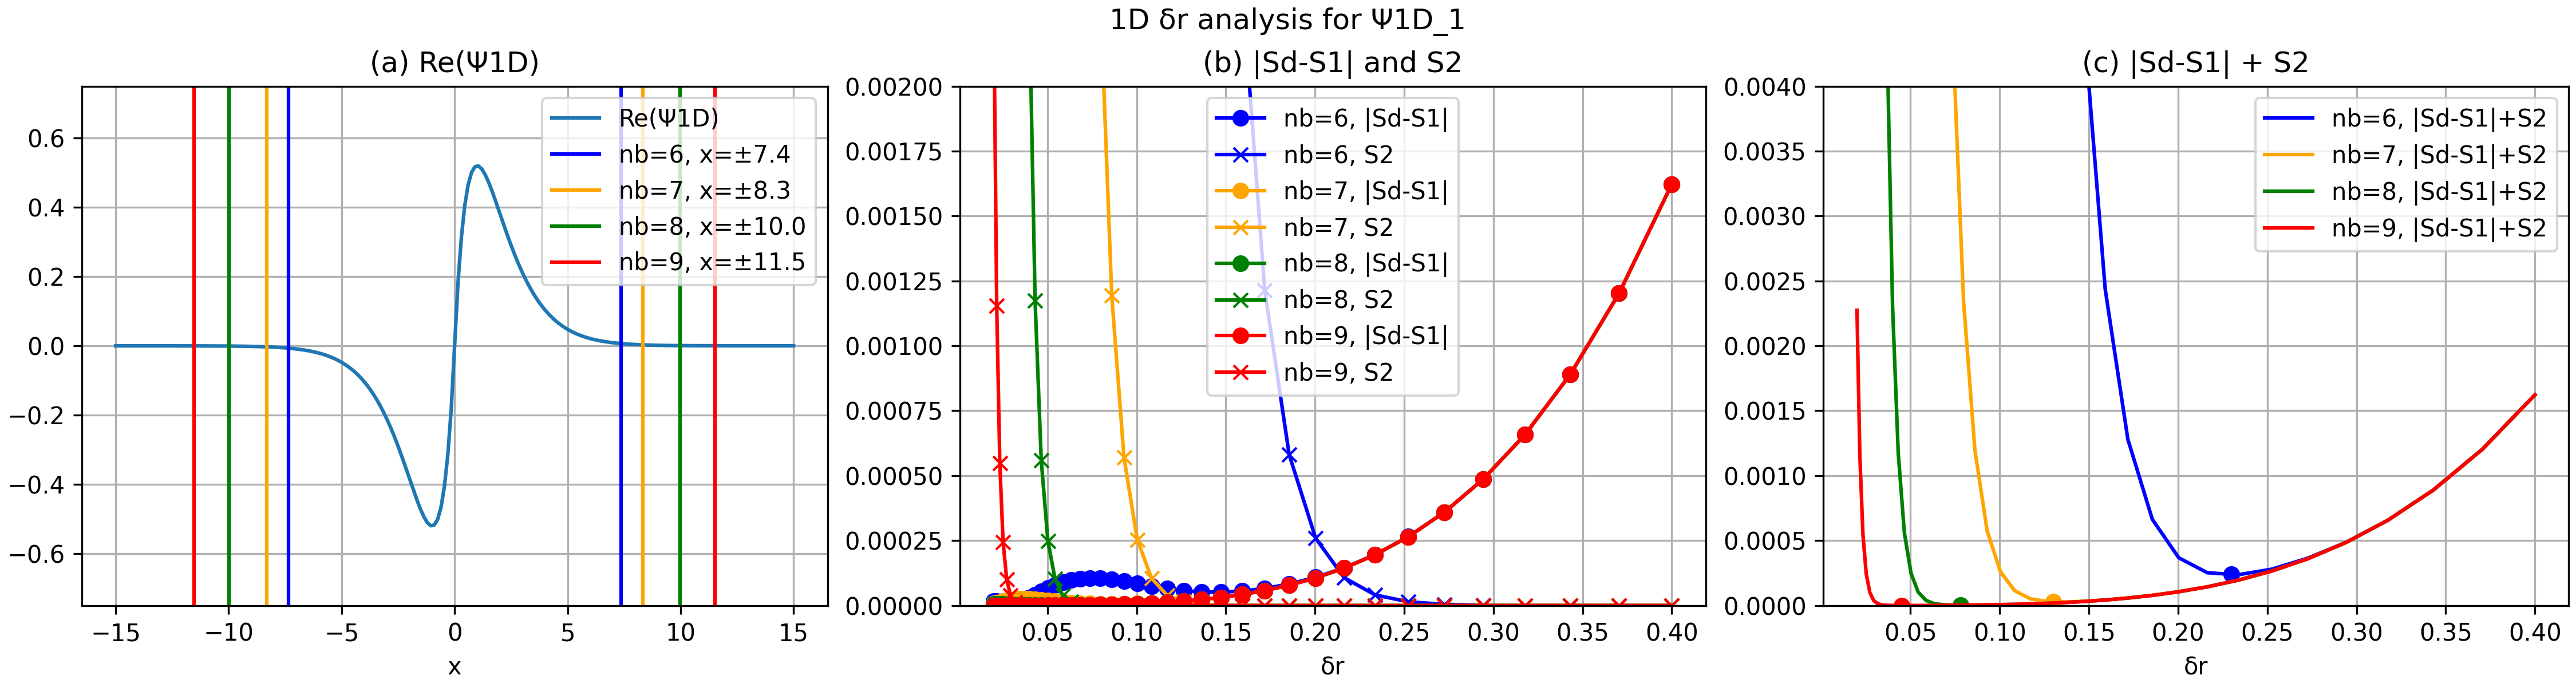
\includegraphics[width=\columnwidth]{paper2025_figs/dq_tradeoff/eval1d_dq.png}
        \caption{1次元モデル $\PsiOneD_1$}
        \label{subfig:dq-tradeoff-1d}
    \end{subfigure}
    \begin{subfigure}{1.0\columnwidth}
        \centering
        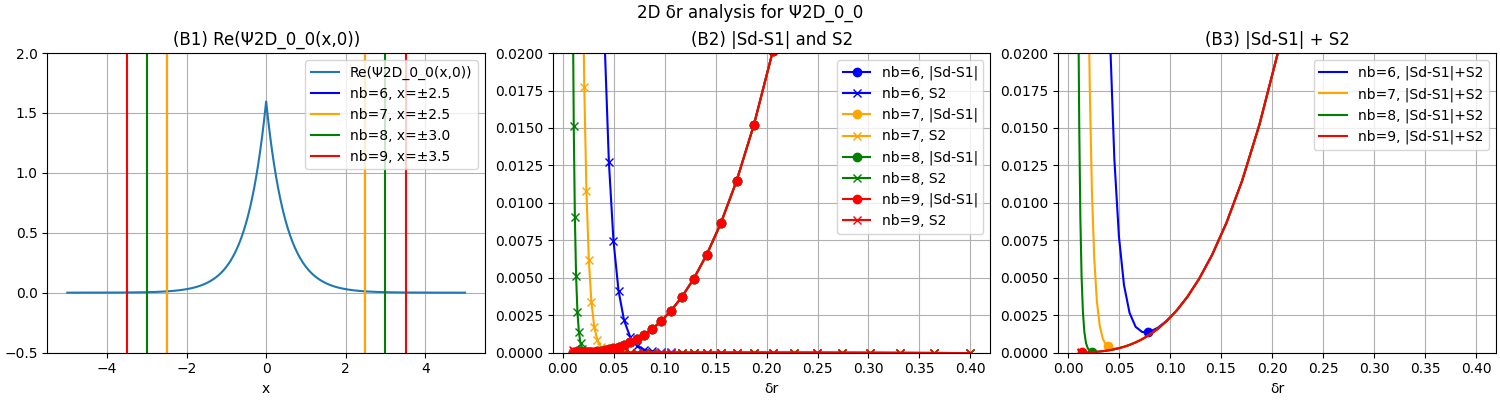
\includegraphics[width=\columnwidth]{paper2025_figs/dq_tradeoff/eval2d_dq_geom_0_0.png}
        \caption{2次元モデル $\PsiTwoD_{0,0}$}
        \label{subfig:dq-tradeoff-2d-0-0}
    \end{subfigure}
    \begin{subfigure}{1.0\columnwidth}
        \centering
        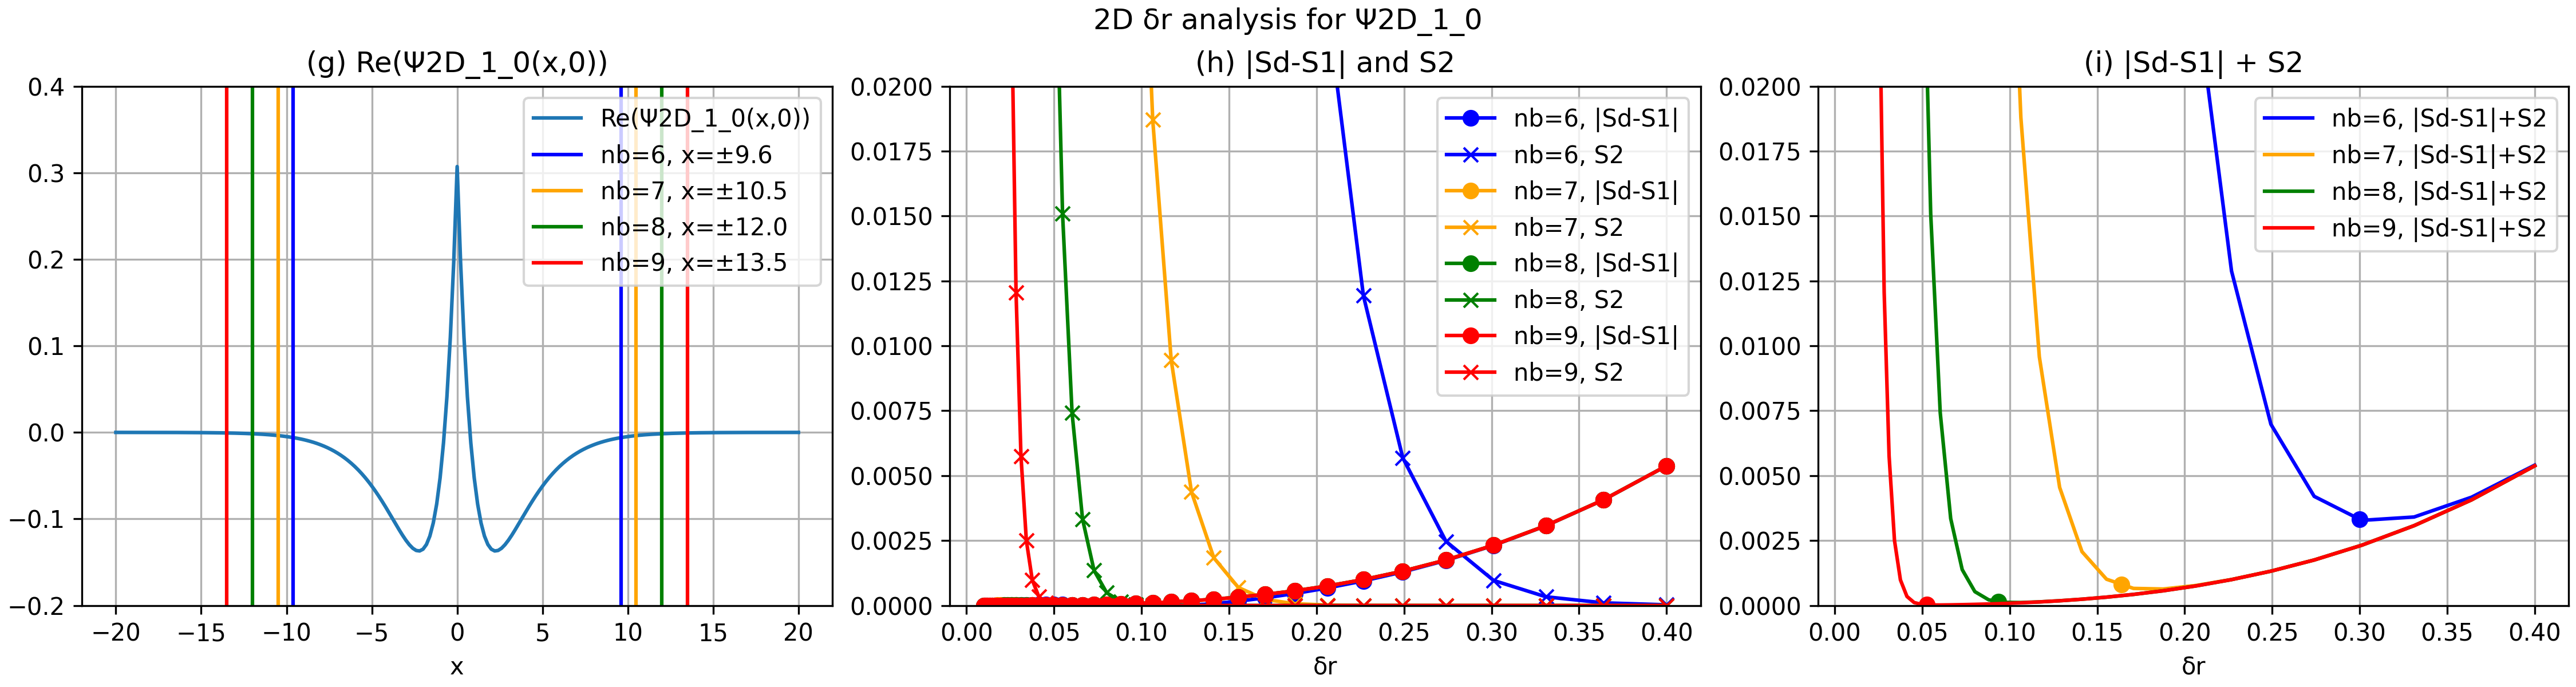
\includegraphics[width=\columnwidth]{paper2025_figs/dq_tradeoff/eval2d_dq_geom_1_0.png}
        \caption{2次元モデル $\PsiTwoD_{1,0}$}
        \label{subfig:dq-tradeoff-2d-1-0}
    \end{subfigure}
    \caption{いくつかの $\nb$ における$|\Sd-S_1|$と$S_2$の関係}
    \label{fig:dq-tradeoff}
    \begin{flushleft}\small

        (a)は1次元の $\PsiOneD_1$ に関するグラフ。(b), (c)はそれぞれ2次元の
        $\PsiTwoD_{0,0},\PsiTwoD_{1,0}$ に関するグラフ。(A1)から(C1)は波動関数
        の$y=0$切片における実部の値を示しており、選ばれた$\deltar$に対する
        $\pm L/2$の位置が垂直線で示されている。(A2)から(C2)は        
        $|\Sd-S_1|$と
        $S_2$を別の線としてプロットしており(式\eqref{eq:err-disc-definition},
        \ref{eq:err-cutoff-definition})、(A3)から(C3)が両者の和をプロットしてい
        る。誤差の和が最小となる点がトレードオフが均衡する点であり、最適な
        $\deltar$の値である。

    \end{flushleft}
\end{figure}
\clearpage

\subsection{δtの決定方法}
\label{subsec:deltat-selection-method}
\subsubsection{サンプリング定理に基づくδtの条件}
\label{subsubsec:deltat-selection-by-sampling-theorem}
$\deltat$が満たすべき条件の根拠としては、サンプリング定理に由来する条件
と、Trotter分解の誤差に由来した条件がある。まず、サンプリング定理に基づく条件に
ついて検討する。

Trotter分解による時間発展によって求まる波動関数の各ステップでの値をサンプリング
された信号ととらえると、サンプリング定理により信号の中の最も高い周波数成分の２倍
のサンプリング周波数、すなわち $1/\deltat$ よりも高い周波数を用いる必要があ
る。Suzuki-Trotter分解の計算の文脈ではポテンシャルエネルギー項と運動エネルギー項
のそれぞれにおいて、時間発展の１ステップでの位相の変化量が半周期分、すなわち$\pi$
以下であることを意味する。
\begin{align}
\max_{\bm{r}}\abs{\Hep(\bm{r})\deltat/\hbar} < \pi \label{eq:nyqist-limit-by-hep}\\
\max_{\bm{k}}\abs{\Hek(\bm{k})\deltat/\hbar} < \pi \label{eq:nyqist-limit-by-hek}
\end{align}
それぞれの式は、波動関数が所与の条件下では以下のように具体的に求めることができる。

まず、本報告の１次元モデルの場合について検討する。位置エネルギー項に関する不等式
\ref{eq:nyqist-limit-by-hep}を解こうとした場合、そのままでは極において$\Hep$が
発散してしまう。時間発展計算においては、発散を起こさないように$\Hep$に近似を導入す
るので、その近似式を用いて評価する。

クーロンポテンシャルの極の扱いの節で述べたように1次元モデルにおけるハミルトニア
ンの近似式は$\HaOne(r)$で$\Delta_1=\deltar/2$ と置いたものである。格子点座標につ
いて記述すると
\begin{equation}
\HaOneOneD(\chij) = \begin{cases}
-\frac{1}{\abs{\chij}} & (\chij\neq0) \\
-\frac{2}{\deltar} & (\chij=0)
\end{cases}
\end{equation}
である。$\abs{\HaOneOneD}$が最大となるのは $\chij=0$ の時であり、
\begin{equation}
\max_{j}\abs{\Hep(\chij)} = \frac{2\deltat}{\deltar\hbar}<\pi
\end{equation}
となる。これを$\deltat$について解くと、
\begin{equation}
\deltat < \frac{\pi\deltar\hbar}{2}=\frac{L\pi\hbar}{2^{\nb+1}}\equiv\deltatPmaxOneD
 \label{eq:nyqist-limit-by-hep-final}
\end{equation}
を得る。ここで、$\deltar=L/2^{\nb}$を用いた。

同様に、運動エネルギー項に関する不等式\eqref{eq:nyqist-limit-by-hek}からは、
\begin{equation}
\max_{\ell}\abs{\frac{\hbar^2(\kellx)^2}{2}\cdot\frac{\deltat}{\hbar}} < \pi
\label{eq:nyqist-limit-by-hek-maximum}
\end{equation}
が得られる。波数$\kaplx$の絶対値が最大となるのは波数のインデクス
$\ell=\kaplx=-2^{\nb-1}$の時でありその時の
$\kellx=\kaplx\deltak=(-2^{\nb-1})\times2\pi/L$となる。これを用いると式\eqref{eq:nyqist-limit-by-hek-maximum}は、
\begin{equation}
    \frac{\hbar^2}{2}\left(\frac{2\pi}{L}\cdot 2^{(\nb-1)}\right)^2\cdot\frac{\deltat}{\hbar} < \pi
\end{equation}
となり、これを$\deltat$について解くと
\begin{equation}
\deltat < \frac{L^2}{2^{2\nb-1}\hbar\pi}\equiv\deltatKmaxOneD
 \label{eq:nyqist-limit-by-hek-final}
\end{equation}
となる。時間発展の期間$T$とTrotter分割数 $\nT$を用いると $\deltat=T/\nT$ となること
から、$\deltat$に関するこれらの上限値に対応する分割数の下限値をそれぞれ
\begin{align}
    \nTpminOneD &= \frac{T}{\deltatPmaxOneD}=\frac{2^{\nb+1}T}{L\pi\hbar}
    \label{eq:nT-pmin-definition}\\
    \nTkminOneD &= \frac{T}{\deltatKmaxOneD}=\frac{2^{2\nb-1}\pi\hbar T}{L^2}
    \label{eq:nT-kmin-definition}
\end{align}
と定める。時間発展の分割数$\nT$はこれらのいずれよりも大きい値にする必要がある。

次に２次元モデルについて同様に検討する。

まず位置エネルギー項に基づく不等式\eqref{eq:nyqist-limit-by-hep}については、2次元
モデルにおいても1次元モデルと同様に極における発散を防ぐために $\Hep$ には近似式
を用いる。次節で検討するように２つの近似式 $\HaOne$,\ $\HaTwo$ のパラメータ
$\Delta_1,\Delta_2$ には共通の$\deltar/4$ を用いる。格子点座標に基づいて書くと
\begin{align}
\HaOneTwoD(\chij) &= \begin{cases}
    -\frac{1}{\abs{\chij}} & (\chij\neq0) \\
    -\frac{4}{\deltar} & (\chij=0)
\end{cases}\\
\HaTwoTwoD(\chij) &= -\frac{1}{\sqrt{\abs{\chij}^2+(\deltar/4)^2}}
\end{align}
これらを用いると式\eqref{eq:nyqist-limit-by-hep} の最大値は等しく
\begin{equation}
\max_{j}\abs{\HaOneTwoD(\chij)\deltat/\hbar}
  = \max_{j}\abs{\HaTwoTwoD(\chij)\deltat/\hbar}
  = \frac{4\deltat}{\deltar\hbar} < \pi
\end{equation}
となり、これより
\begin{equation}
\deltat < \frac{\pi\deltar\hbar}{4}
        =\frac{L\pi\hbar}{2^{\nb+2}}
        \equiv\deltatPmaxTwoD
 \label{eq:nyqist-limit-by-hep-final-2D}
\end{equation}
を得る。

運動エネルギー項に基づく不等式\eqref{eq:nyqist-limit-by-hek}からは、
\begin{equation}
\max_{\ell}\abs{\frac{\hbar^2((\kellx)^2+(\kelly)^2)}{2}\cdot\frac{\deltat}{\hbar}} < \pi
\label{eq:nyqist-limit-by-hek-maximum-2D}
\end{equation}
波数$\kellx,\kelly$ の二乗和が最大となるのは $\kaplx=\kaply=-2^{\nb-1}$の時であ
り、その時の $\kellx=\kelly=\kaplx\deltak=\kaply\deltak=-2^{\nb-1}\times2\pi/L$ を
用いると式\eqref{eq:nyqist-limit-by-hek-maximum-2D}は、
\begin{equation}
\frac{\hbar^2}{2}\cdot2\left(-\frac{2^{\nb-1}2\pi}{L}\right)^2\cdot\frac{\deltat}{\hbar}<\pi
\end{equation}
すなわち、
\begin{equation}
\deltat < \frac{L^2}{2^{2\nb}\hbar\pi} \equiv\deltatKmaxTwoD
 \label{eq:nyqist-limit-by-hek-final-2D}
\end{equation}
を得る。これに対応するTrotter分割数の下限値はそれぞれ
\begin{align}
    \nTpminTwoD &= \frac{T}{\deltatPmaxTwoD}=\frac{2^{\nb+2}T}{L\pi\hbar} \\
    \nTkminTwoD &= \frac{T}{\deltatKmaxTwoD}=\frac{2^{2\nb}\pi\hbar T}{L^2}
\end{align}
となる。

\subsubsection{Trotter誤差に基づくδtの条件}
\label{subsec:deltat-selection-by-trotter-error}
Trotter分解ではハミルトニアンを運動エネルギー項とポテンシャルエネルギー項に分け
て$e^{-it(H_1+H_2)/\hbar}\simeq\left(e^{-i{tH}_1/N}e^{-itH_2/N}\right)^N$と近似
することに起因して誤差が生じる。旧来のTrotter誤差評価では2つのハミルトニアンの交
換子のオペレータノルム $\| [H_1,H_2] \|$ すなわち
$\sup_{\|\psi\|=1}\|(H_1H_2-H_2H_1)\psi\|$ に基づいて誤差の上限を見積もる。この手法は
最大の誤差をもたらす波動関数 $\psi$ に基づいて評価するワーストケース評価となって
おり、誤差を過大に評価することが指摘されている
\cite{Childs2021.PhysRevX.11.011020}。より厳密な誤差推定を実現するために、実際に
計算対象とする波動関数を仮定した状態依存の誤差評価をすることが提案されている
\cite{Burgarth2024.PhysRevResearch.6.043155}。ここでは、この提案に従い状態依存の
Trotter誤差評価に基づいて検討する。

サンプリング定理に基づく $\deltat$ の決定の場合と異なり、Trotterの誤差評価式から
は特定の$\deltat$ の値が上限値として求まることはなく、$\deltat$ と誤差の上限に関
する不等式が得られる。$\left(H_1+H_2\right)\phi=h\phi$ となるようなハミルトニア
ン$H_1+H_2$ の固有値 $h$ の固有関数 $\phi$ を初期値として1次のTrotter分解を用い
て時間発展させたときの誤差は、任意の $g\in\mathbb{R}$ に対して
\begin{equation}
    \xiN{1}(t;\phi)=\left\|\left[\SN{1}(t)-e^{-it(H_1+H_2)/\hbar}\right]\phi\right\|
    \leq\frac{t^2}{2N}\| \left(\|(H_1-g)^2\phi\|+\|(H_2-h+g)^2\phi\|\right)
    \label{eq:observed-trotter-error-1st}
\end{equation}

で与えられる\cite{Burgarth2024.PhysRevResearch.6.043155}。ここで
$\xiN{1}(t;\phi)$は1次のTrotter分解に基づく計算結果として得られた誤差であり、
$S_N^{(1)}$ は一次のTrotter分解に基づく時間発展演算子、すなわち
\begin{equation}
    \SN{1}(t)=\left(e^{-i{tH}_1/N}e^{-itH_2/N}\right)^N
\end{equation}
である。式\eqref{eq:observed-trotter-error-1st}の右辺はの最小値を$\BN{1}$とおく:
\begin{equation}
\BN{1}(t;\phi)=\inf_{g\in\mathbb{R}}\frac{t^2}{2N}
    \left(\|(H_1-g)^2\phi\|+\|(H_2-h+g)^2\phi\|\right)
\label{eq:observed-trotter-error-bound-1st}
\end{equation}
式\eqref{eq:observed-trotter-error-bound-1st} により特定の $t,N$ に対する誤差の上限
を見積もることができ、誤差のオーダーが $O(t^2/N)$ であることを示しており、誤差が
分割数$N$に反比例することを示している。ただし$N$ が小さい条件や空間分解能が高い条件
ではこの式は成り立たず、オーダーは$O(t^2 N^{-1/4})$ なると指摘されている
\cite{Burgarth2024.PhysRevResearch.6.043155}。

二次のTrotter分解を用いた場合の誤差の見積もり式は
\begin{equation}
  \xiN{2}(t;\phi)\leq\frac{t^3}{N^2}\left(\frac{1}{24}\|H_1(g)^3\phi\| + \frac{1}{8}\|H_2(g)H_1(g)^2\phi\|
  +\frac{1}{12}\|H_2(g)^3\phi\|\right)
    \label{eq:observed-trotter-error-2nd}
\end{equation}
となる\cite{Burgarth2024.PhysRevResearch.6.043155}。ここで
$H_1(g)=H_1-g,H_2(g)=H_2-h+g$である。式\eqref{eq:observed-trotter-error-2nd}の右辺
の最小値を$\BN{2}$とおく:
\begin{equation}
\BN{2}(t;\phi)=\inf_{g\in\mathbb{R}}\frac{t^3}{N^2}
    \left(\frac{1}{24}\|H_1(g)^3\phi\| + \frac{1}{8}\|H_2(g)H_1(g)^2\phi\|
  +\frac{1}{12}\|H_2(g)^3\phi\|\right)
\label{eq:observed-trotter-error-bound-2nd}
\end{equation}

式\eqref{eq:error-total-decomposition} が示す異なる種類の誤差の中で $\errtrotter$
の比率が大きい状況においては式\eqref{eq:observed-trotter-error-1st}や
\eqref{eq:observed-trotter-error-2nd}に基づく誤差の改善が期待できる。他方、Trotter
誤差以外の要因の誤差が支配的である条件では$N$を増やしても$O(N^{-1})$ や
$O(N^{-2})$ の誤差縮小は望めない。


時間離散化のパラメータ $\deltat$ には離散的フーリエ変換を用いることによるサンプ
リング定理から上限が決まる（式\eqref{eq:nyqist-limit-by-hep},
\eqref{eq:nyqist-limit-by-hek-final}, \eqref{eq:nyqist-limit-by-hep-final-2D},
\eqref{eq:nyqist-limit-by-hek-final-2D}）。 Trotter誤差は分割数$\nT=t/\deltat$に応
じて誤差の上限が決まる（式\eqref{eq:observed-trotter-error-bound-1st},
\eqref{eq:observed-trotter-error-bound-2nd}）。これら複数の制約の間にはトレードオ
フ関係はないが、式\eqref{eq:error-total-decomposition}で示した全体の誤差は複数の成
分を含むため$\deltat$による誤差が縮小しても$\errtotal$ が殆ど改善しないこともあ
り得る。計算コストの観点では$\deltat$ はなるべく大きな値を使うことが望ましいの
で、改善が見られる範囲で値を小さくすべきである。

時間発展期間$t=1.0$を固定して、Trotter分割数 $\nT$ を変化させた際の誤差の上限
$\BN{\gamma}(\psi;t)$ と誤差の観測値 $\xiN{\gamma}$を図
\ref{fig:trotter-error-t1-part1}, \ref{fig:trotter-error-t1-part2} に示す。
$\gamma=1,2$ はTrotter次数を表す。より長いシミュレーション時間の例として波動関数
$\PsiTwoD_{1,0}$の周期が$2\pi/E_2=28.277$ であることを考慮して $t=30.0$としたグ
ラフを図\ref{fig:trotter-error-t30-part1}, \ref{fig:trotter-error-t30-part2}に示
す。サンプリング定理に基づく$\nT$の下限である $\nTpminTwoD$ と $\nTkminTwoD$を垂
直線で示した。他のグラフの単位がエネルギーであるのに対して、これらのグラフは式
\eqref{eq:observed-trotter-error-1st}, \eqref{eq:observed-trotter-error-2nd}定義した
波動関数の振幅の差のノルムを示している。

Trotter次数 $\gamma$による違いは方位量子数 $m=0$ である $\PsiTwoD_{0,0}$ と
$\PsiTwoD_{1,0}$ の計算例（図 \ref{subfig:trotter-error-2d-0-0-6b-t1} から
\ref{subfig:trotter-error-2d-1-0-9b-t1}）ではほとんど見られなかった。$m=1$ であ
る$\PsiTwoD_{1,1}$では$\nT$ が小さい領域では両者に差が見られた。Burgarthは3次元
の水素原子モデルにおいて方位量子数が0の固有関数ではTrotter次数を上げても精度の改
善は見られないことを報告している\cite{Burgarth2024.PhysRevResearch.6.043155}。次
元は異なるが$\PsiTwoD_{0,0}$と$\PsiTwoD_{1,0}$の計算例は同様の結果を示す。

いずれのグラフも$\nT$の増大と共に$\xiN{1}$, $\xiN{2}$ 共に減少する
が、$\nT=\nTkminTwoD$のあたりで飽和する。$\PsiTwoD_{1,1}$ では $\nT>\nTkminTwoD$
の領域で多少の減少が見られるがわずかである。これは、この領域では空間分解能による
誤差$\errdisc$ の成分が優勢であるためと考えられる。ここに示した波動関数で
は、$\nT$の値を$\nTkminTwoD$よりも大きな値に設定しても誤差の改善はない。例えば図
\ref{subfig:trotter-error-2d-0-0-6b-t1}と図
\ref{subfig:trotter-error-2d-0-0-9b-t1}を比較すると同じ$\PsiTwoD_{0,0}$に対して
$n_b$を6から9に増やすと飽和した時の誤差の値が1/10程度に縮小していることがわか
る。

なお、$\nT$ に対応する$\deltat$ の値を考えると$t=1.0 \mathrm{a.u.}=24.19
\mathrm{attosecond} (\mathrm{as})$ をさらに$10^2$から$10^3$期間に分割するため
attosecond未満の値になる。

\begin{figure}[ht]
    \centering
    \begin{subfigure}{0.45\columnwidth}
        \centering
        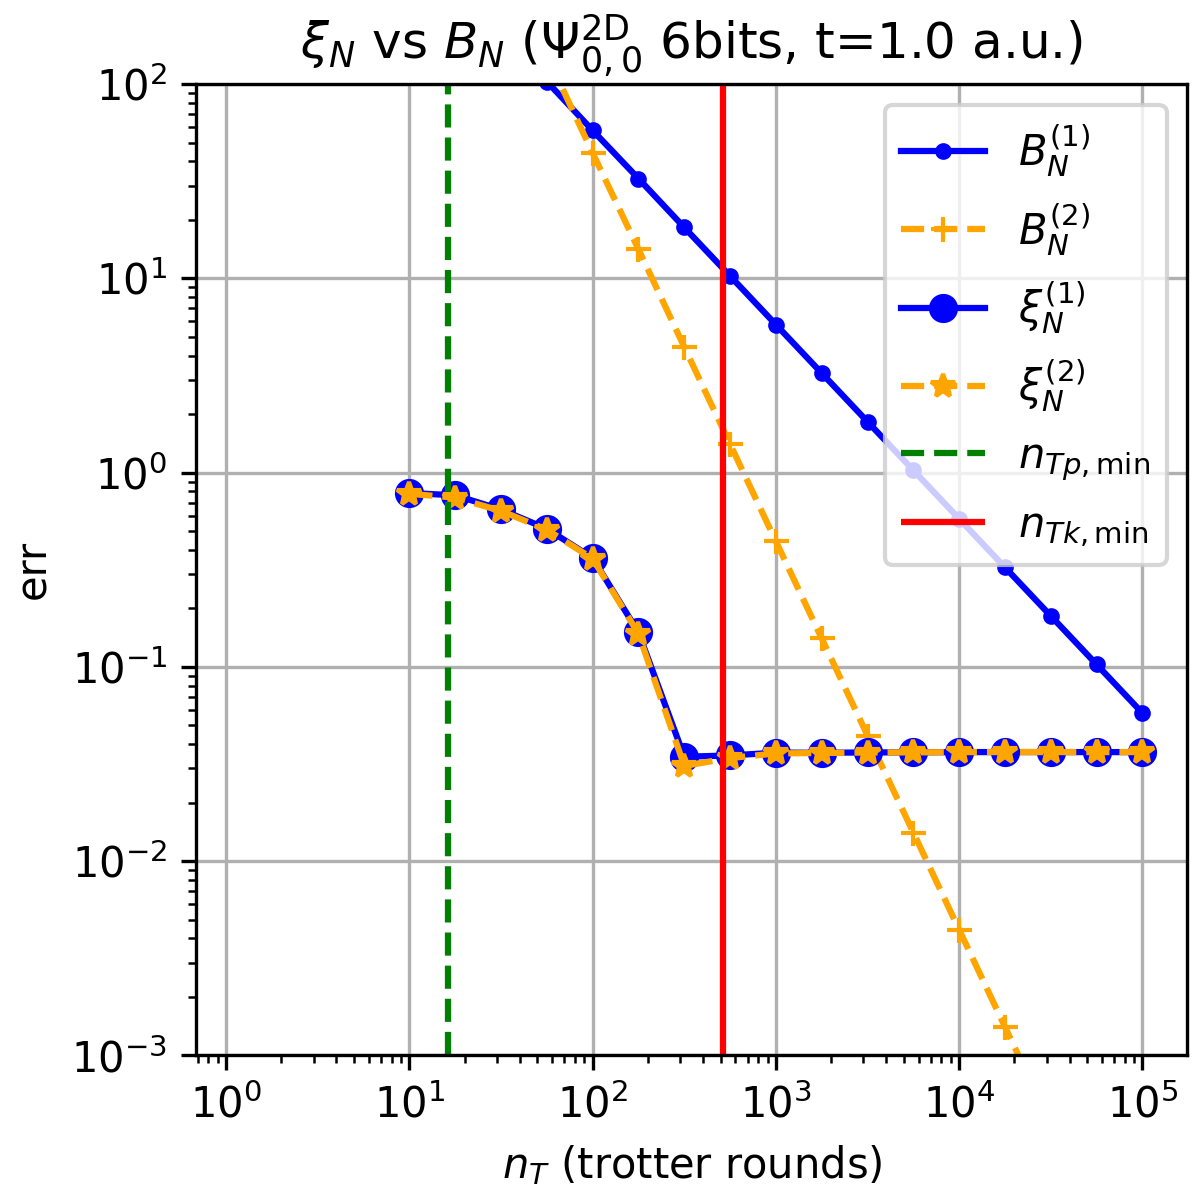
\includegraphics[width=1\columnwidth]{paper2025_figs/sdt_error/trotter_err_n0_m0_6b_t1.0.png}
        \caption{$\PsiTwoD_{0,0}, \nb=6, t=1.0$}
        \label{subfig:trotter-error-2d-0-0-6b-t1}
    \end{subfigure}
    \begin{subfigure}{0.45\columnwidth}
        \centering
        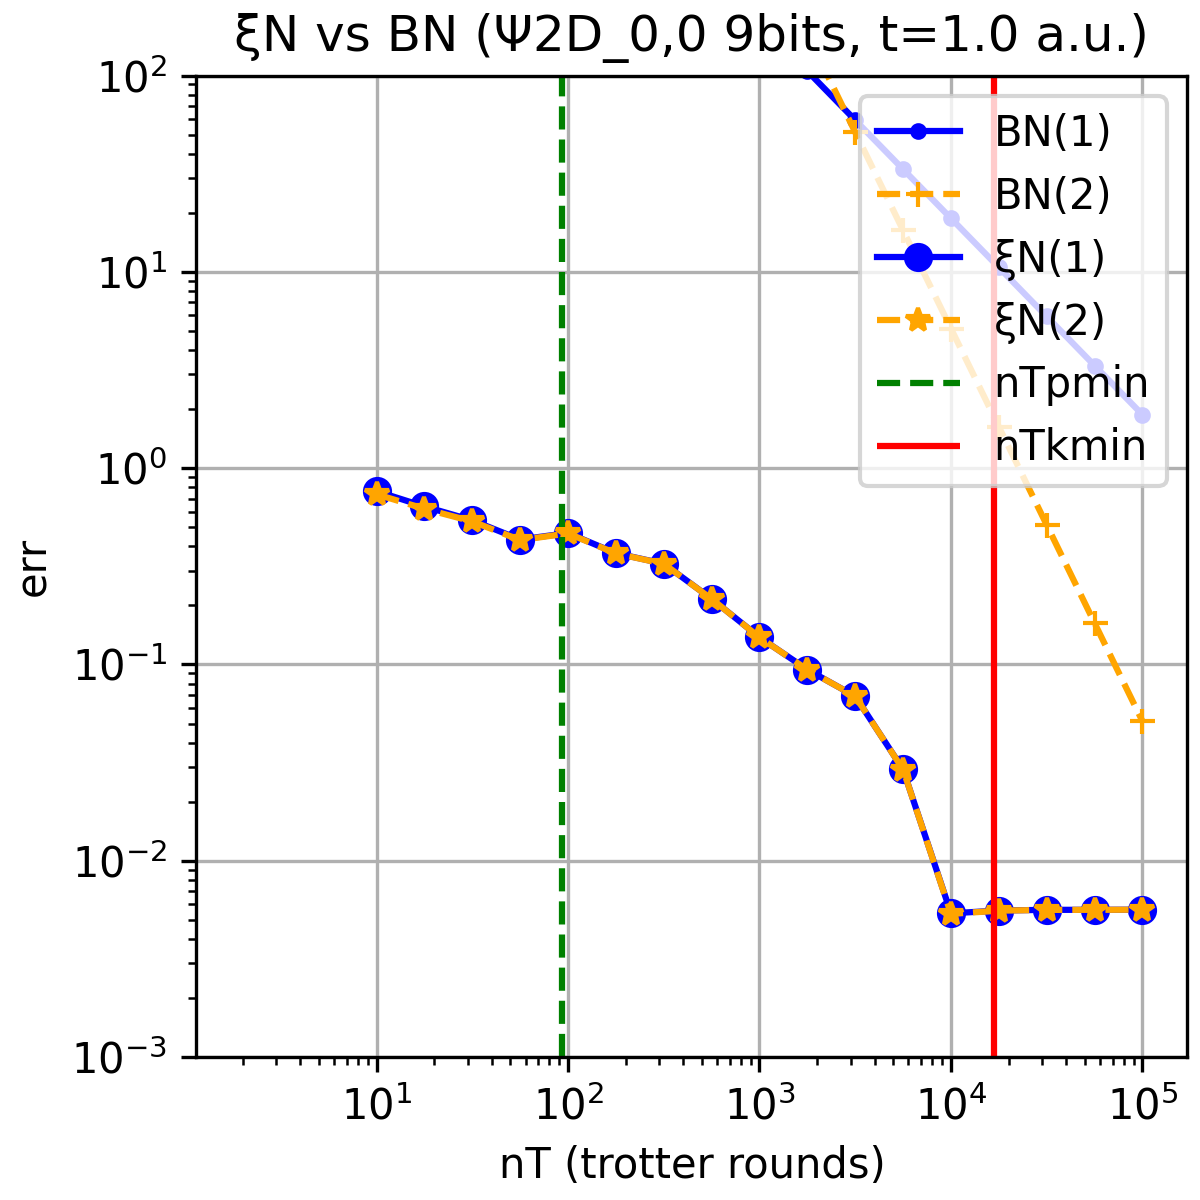
\includegraphics[width=1\columnwidth]{paper2025_figs/sdt_error/trotter_err_n0_m0_9b_t1.0.png}
        \caption{$\PsiTwoD_{0,0}, \nb=9, t=1.0$}
        \label{subfig:trotter-error-2d-0-0-9b-t1}
    \end{subfigure}

    \begin{subfigure}{0.45\columnwidth}
        \centering
        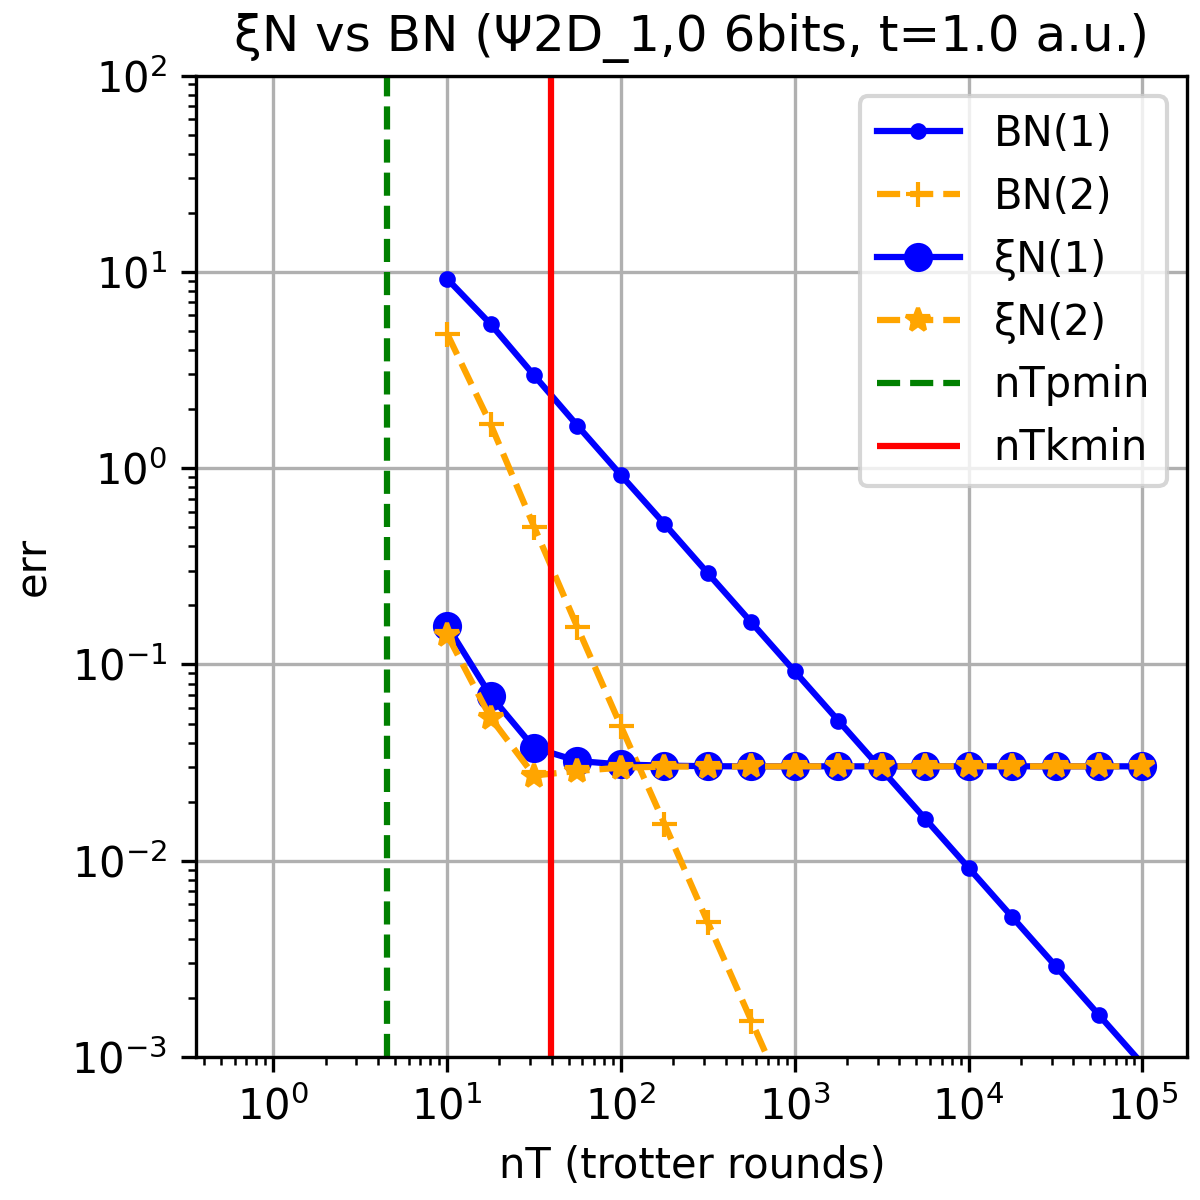
\includegraphics[width=1\columnwidth]{paper2025_figs/sdt_error/trotter_err_n1_m0_6b_t1.0.png}
        \caption{$\PsiTwoD_{1,0}, \nb=6, t=1.0$}
        \label{subfig:trotter-error-2d-1-0-6b-t1}
    \end{subfigure}
    \begin{subfigure}{0.45\columnwidth}
        \centering
        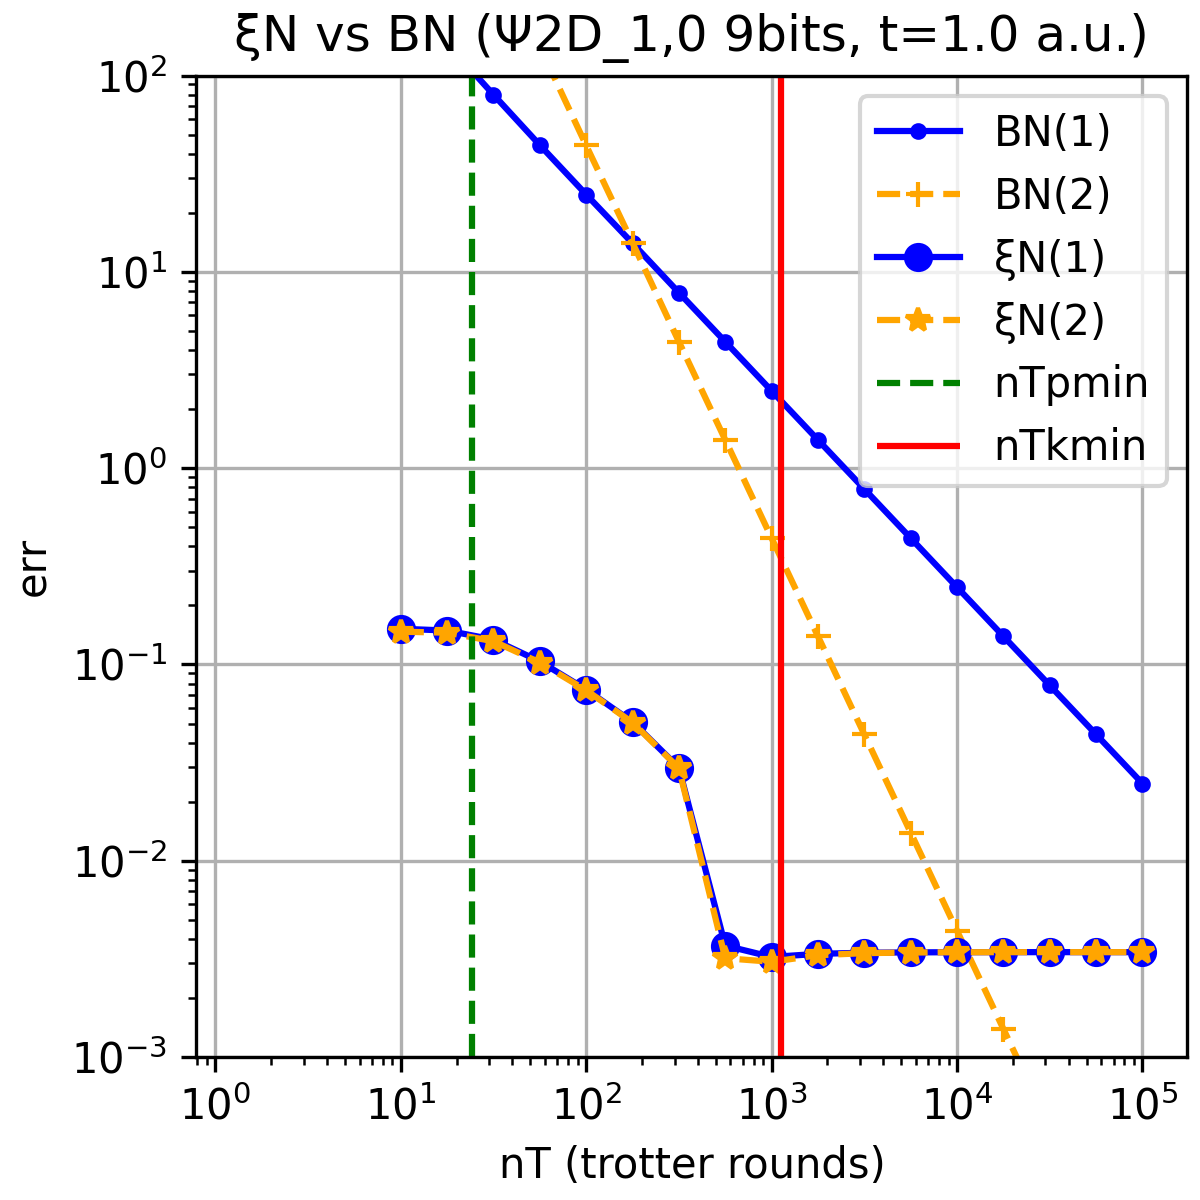
\includegraphics[width=1\columnwidth]{paper2025_figs/sdt_error/trotter_err_n1_m0_9b_t1.0.png}
        \caption{$\PsiTwoD_{1,0}, \nb=9, t=1.0$}
        \label{subfig:trotter-error-2d-1-0-9b-t1}
    \end{subfigure}

    \caption{時間発展期間$t=1.0$ での分割数$\nT$に対する誤差の上限 $\BN{\gamma}$ と観測値 $\xiN{\gamma}$}
    \label{fig:trotter-error-t1-part1}
    \begin{flushleft}\small

        2次元モデルの波動関数におけるTrotter分割数に対する誤差。時間発展の期間
        $t=1.0$は固定であり、横軸はTrotter分割数$\nT$である。$\xiN{1}$と
        $\xiN{2}$はそれぞれTrotter次数1,2 に対する誤差である（式
        \eqref{eq:observed-trotter-error-1st},
        \eqref{eq:observed-trotter-error-2nd}）。この値はTrotter誤差以外の誤差も含
        む。$\BN{1}, \BN{2}$ はそれぞれTrotter誤差の解析的な上限値である（式
        \eqref{eq:observed-trotter-error-bound-1st},
        \eqref{eq:observed-trotter-error-bound-2nd}）。垂直線$\nT=\nTpminTwoD$と
        $\nT=\nTkminTwoD$ はそれぞれ、サンプリング定理に基づく$\deltat$に関する上限
        値 $\deltatPmaxTwoD$と$\deltatKmaxTwoD$ に相当するTrotter分割数である
        （式\eqref{eq:nT-pmin-definition}, \eqref{eq:nT-kmin-definition}）。

    \end{flushleft}
\end{figure}

\begin{figure}[ht]
    \centering
    \begin{subfigure}{0.45\columnwidth}
        \centering
        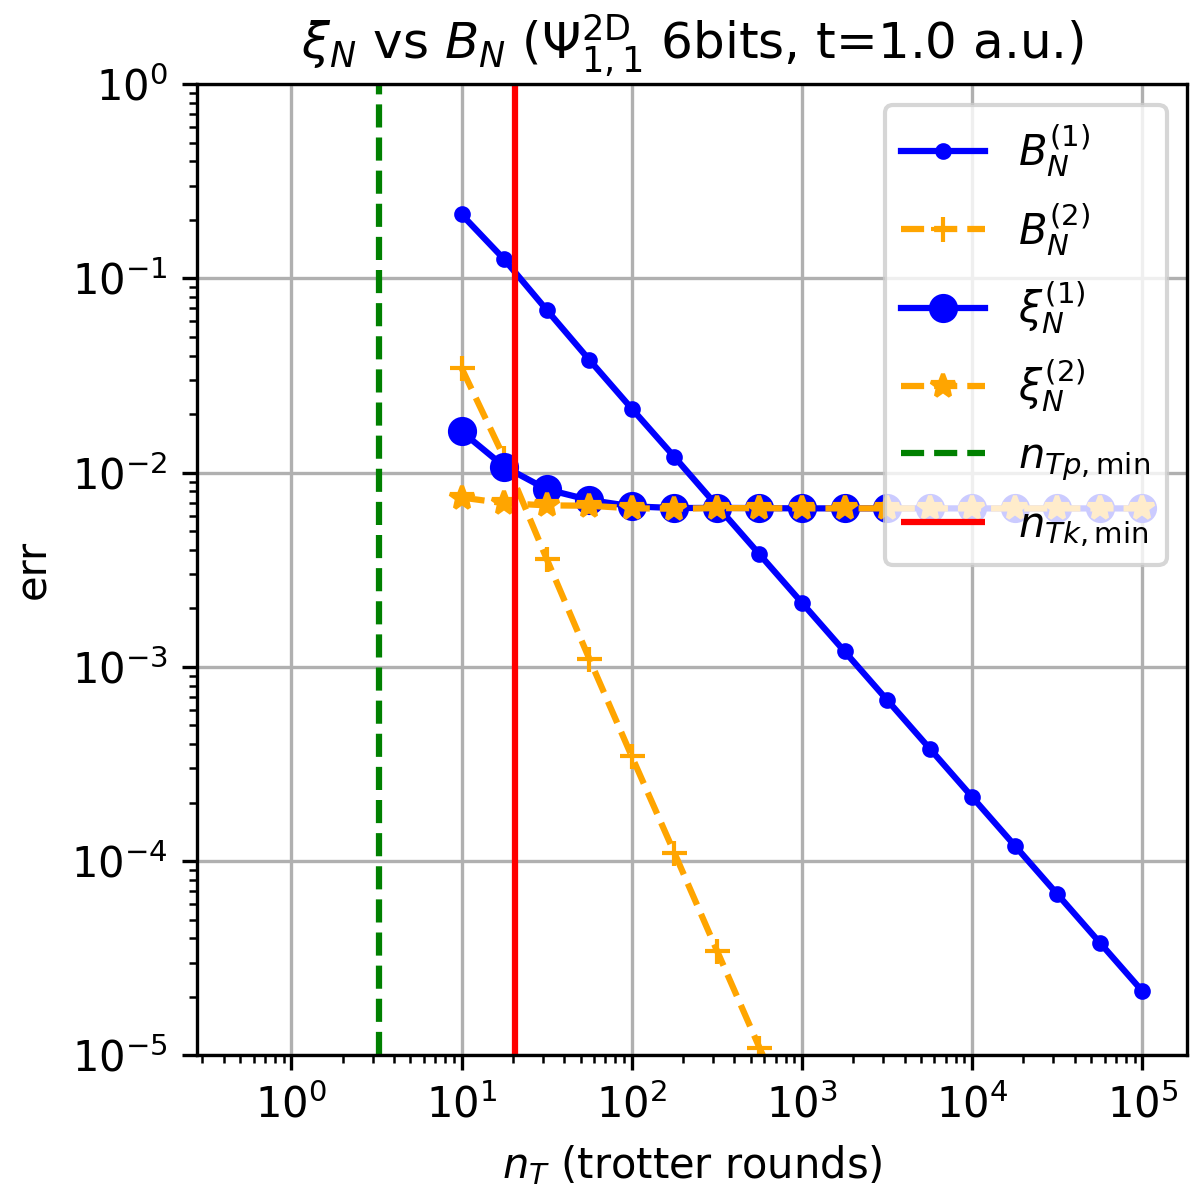
\includegraphics[width=1\columnwidth]{paper2025_figs/sdt_error/trotter_err_n1_m1_6b_t1.0.png}
        \caption{$\PsiTwoD_{1,1}, \nb=6, t=1.0$}
        \label{subfig:trotter-error-2d-1-1-6b-t1}
    \end{subfigure}
    \begin{subfigure}{0.45\columnwidth}
        \centering
        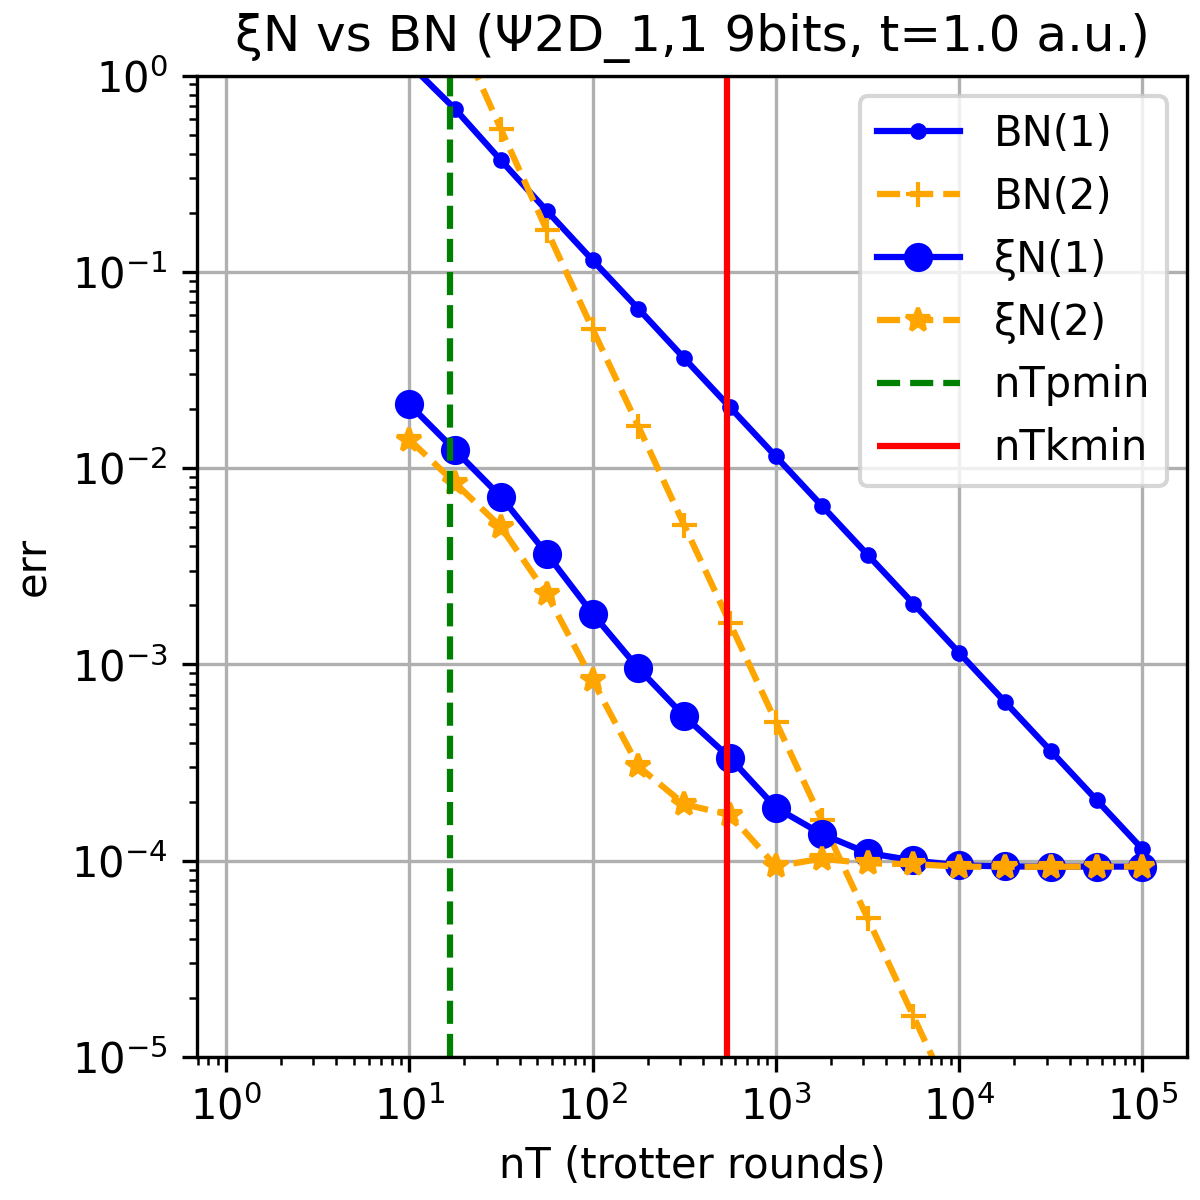
\includegraphics[width=1\columnwidth]{paper2025_figs/sdt_error/trotter_err_n1_m1_9b_t1.0.png}
        \caption{$\PsiTwoD_{1,1}, \nb=9, t=1.0$}
        \label{subfig:trotter-error-2d-1-1-9b-t1}
    \end{subfigure}
    \caption{時間発展期間$t=1.0$ での分割数$\nT$に対する誤差の上限 $\BN{\gamma}$ と観測値 $\xiN{\gamma}$}
    \label{fig:trotter-error-t1-part2}
    \begin{flushleft}\small

        2次元モデルの波動関数におけるTrotter分割数に対する誤差（つづき）。
    \end{flushleft}
\end{figure}

\begin{figure}[ht]
    \centering
    \begin{subfigure}{0.45\columnwidth}
        \centering
        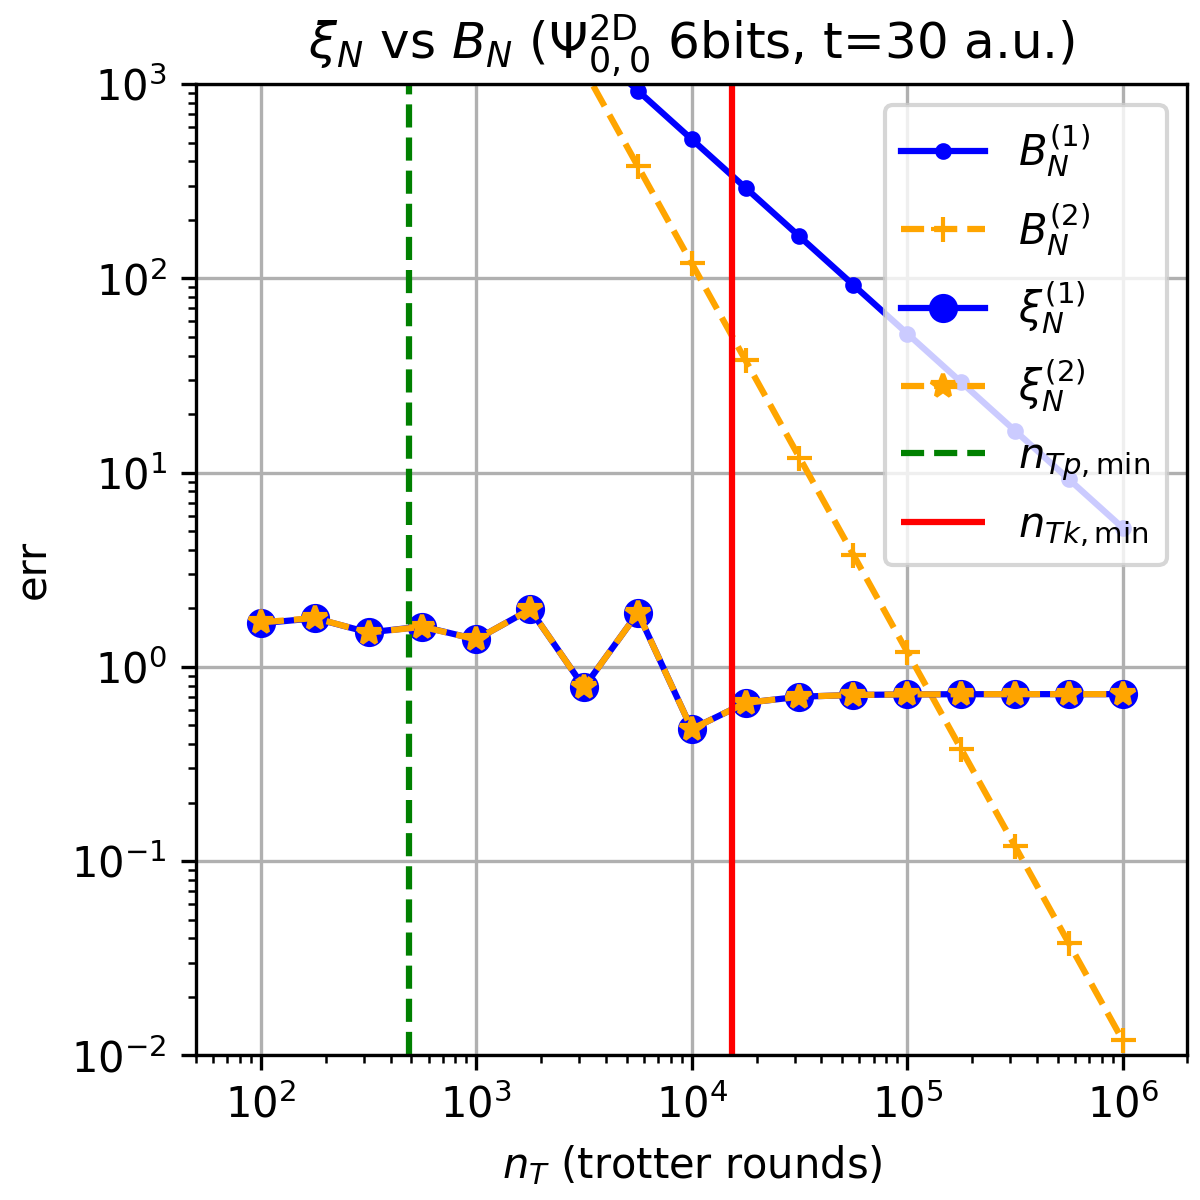
\includegraphics[width=1\columnwidth]{paper2025_figs/sdt_error/trotter_err_n0_m0_6b_t30.png}
        \caption{$\PsiTwoD_{0,0}, \nb=6, t=30.0$}
        \label{subfig:trotter-error-2d-0-0-6b-t30}
    \end{subfigure}
    \begin{subfigure}{0.45\columnwidth}
        \centering
        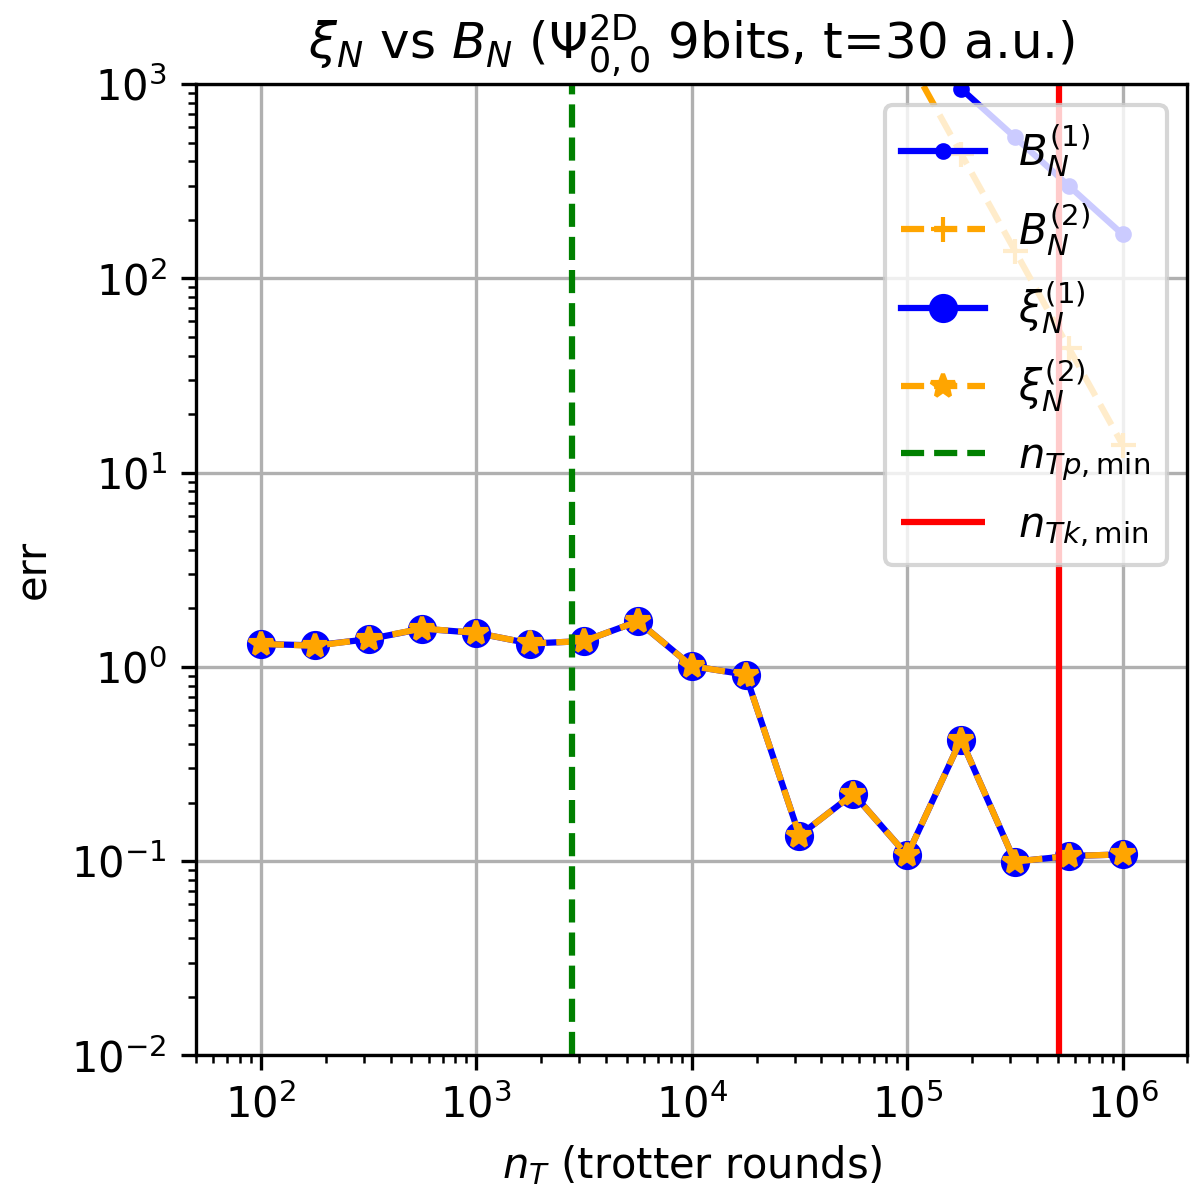
\includegraphics[width=1\columnwidth]{paper2025_figs/sdt_error/trotter_err_n0_m0_9b_t30.png}
        \caption{$\PsiTwoD_{0,0}, \nb=9, t=30.0$}
        \label{subfig:trotter-error-2d-0-0-9b-t30}
    \end{subfigure}

    \begin{subfigure}{0.45\columnwidth}
        \centering
        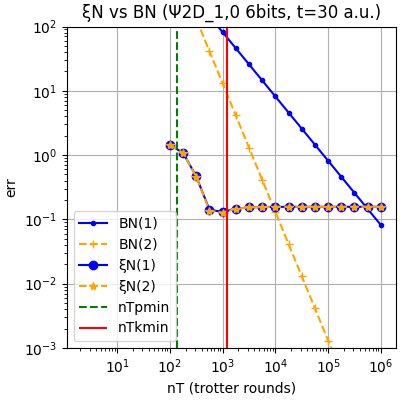
\includegraphics[width=1\columnwidth]{paper2025_figs/sdt_error/trotter_err_n1_m0_6b_t30.png}
        \caption{$\PsiTwoD_{1,0}, \nb=6, t=30.0$}
        \label{subfig:trotter-error-2d-1-0-6b-t30}
    \end{subfigure}
    \begin{subfigure}{0.45\columnwidth}
        \centering
        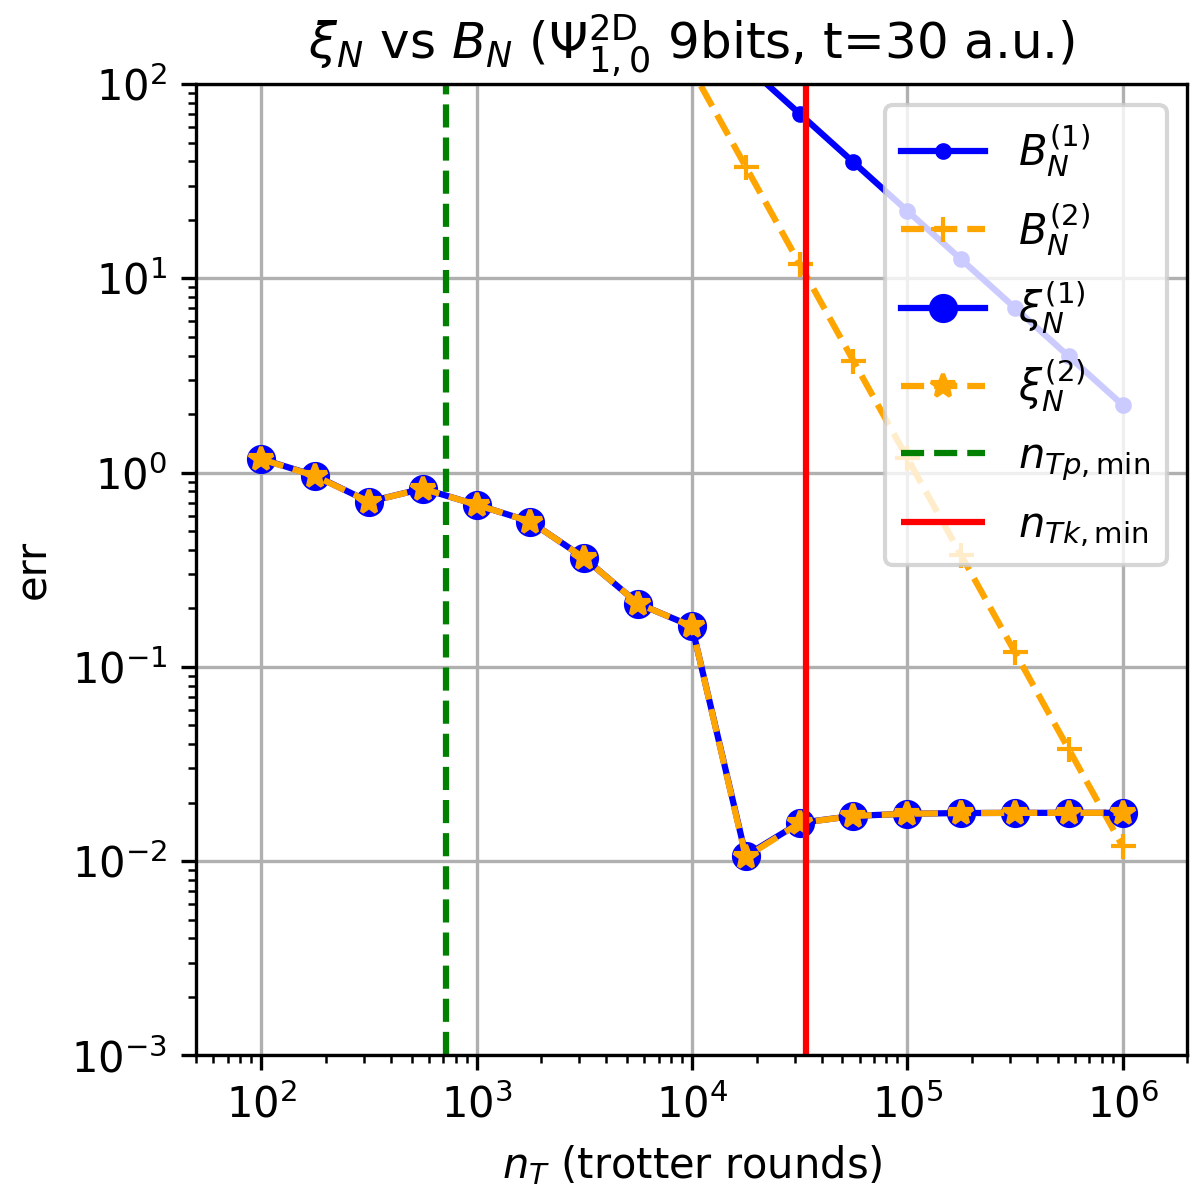
\includegraphics[width=1\columnwidth]{paper2025_figs/sdt_error/trotter_err_n1_m0_9b_t30.png}
        \caption{$\PsiTwoD_{1,0}, \nb=9, t=30.0$}
        \label{subfig:trotter-error-2d-1-0-9b-t30}
    \end{subfigure}

    \caption{時間発展期間$t=30.0$ での分割数$\nT$に対する誤差の上限 $\BN{\gamma}$ と観測値 $\xiN{\gamma}$}
    \label{fig:trotter-error-t30-part1}
\end{figure}

\begin{figure}[ht]
    \centering
    \begin{subfigure}{0.45\columnwidth}
        \centering
        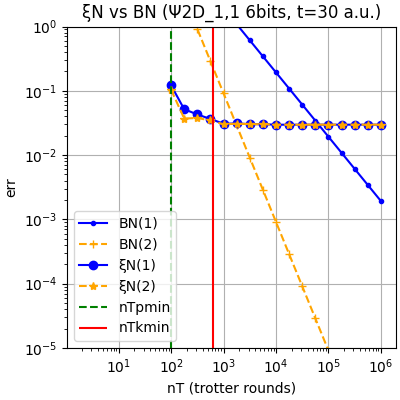
\includegraphics[width=1\columnwidth]{paper2025_figs/sdt_error/trotter_err_n1_m1_6b_t30.png}
        \caption{$\PsiTwoD_{1,1}, \nb=6, t=30.0$}
        \label{subfig:trotter-error-2d-1-1-6b-t30}
    \end{subfigure}
    \begin{subfigure}{0.45\columnwidth}
        \centering
        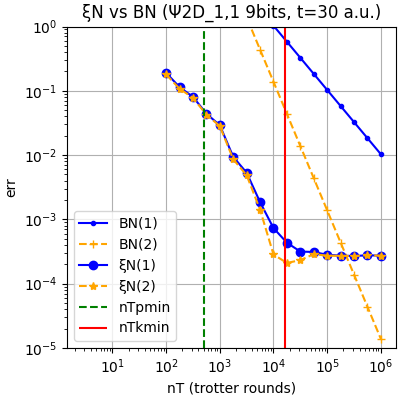
\includegraphics[width=1\columnwidth]{paper2025_figs/sdt_error/trotter_err_n1_m1_9b_t30.png}
        \caption{$\PsiTwoD_{1,1}, \nb=9, t=30.0$}  
        \label{subfig:trotter-error-2d-1-1-9b-t30}
    \end{subfigure}

    \caption{時間発展期間$t=30.0$ での分割数$\nT$に対する誤差の上限 $\BN{\gamma}$ と観測値 $\xiN{\gamma}$（つづき）}
    \label{fig:trotter-error-t30-part2}
\end{figure}
\clearpage

\section{結論}
本研究では、2次元水素原子モデルを対象に、Qiskitエミュレータ上で全系の時間発展が
可能な回路構成を示した。これは、調べた限りにおいてグリッド法に基づく時間発展計算
をクーロンポテンシャルの計算を含めて量子回路で初めて実装し、エミュレータ上で動作
させた例である。

クーロンポテンシャルの特異点を扱う方法として、極を含む格子においては粒子間座標
$r$の代表値として2次元モデルにおいては$r_{\mathrm{eff}}=\delta r/4$ を用いるこ
とを提案した。行った数値評価の範囲ではこの値で誤差が最小となった。

与えられたqubit数の下で誤差を最小化するためには格子間隔 δr を空間離散化誤差とカット
オフ誤差のトレードオフから定めることを提案した。また、トロッター分解の時間刻み
δt は、波動関数の運動量表現における最大の周波数成分の時間変化の速さに着目したサ
ンプリング定理の要請に基づいて決めることができることを数値評価の範囲で確認した。
また、対象の波動関数が基底状態の場合には上記の制約を満たせば残りの誤差はトロッ
ター誤差よりも他の誤差が支配的であった。

これらの知見はグリッド法を用いたシミュレーション条件の設定において有用な指針とな
ると考える。


\printbibliography[heading=bibintoc, title={参考文献}]

%%%%%%%%%%%%%%%% 付録

\appendix
\section{ポテンシャルの近似式のΔ1の導出}
\label{chap:appendix_derivation_derivation}

第\ref{sec:coulomb-potential-handling}節で述べた近似式 $HaOne(r)$ におけるパラメータ $\Delta_1$
の導出を示す。

まず、$\PsiTwoD_{0,0}$に関するパラメタ$\Delta_{1,0,0}$についての式\eqref{eq:delta-1-0-0}の導出を示す。

積分 $W_{0,0}$ は、
\begin{align}
  W_{0,0}
   &= \int_{r=0}^{\deltar/2}\int_{\theta=0}^{2\pi}
      \Hep(r)\abs{\Psi2D_{0,0}(r)}^2rd\theta dr\notag\\
   &= \int_{r=0}^{\deltar/2}\int_{\theta=0}^{2\pi}
      -\frac{1}{r}\left(\frac{q_0^3(0-\abs{0})!}{\pi(0+\abs{0})!}\right)
      (2q_0r)^{2\abs{0}}\exp(-2q_0r)
      \left[L_{0-\abs{0}}^{2\abs{0}}(2q_0r)\right]^2 rd\theta dr\notag\\
   &= -2\pi\int_{r=0}^{\deltar/2}\frac{q_0^3}{\pi}\frac{1}{r}e^{-2q_0r}r\ dr=-2q_0^3
      \left[-\frac{1}{2q_0}e^{-2q_0r}\right]_{0}^{\deltar/2}\notag\\
   &=-q_0^2(-e^{-q_0\deltar}+1)
\end{align}
となる。これに対して $W_{0,0}^\prime$ は、
\begin{align}
    W_{0,0}^\prime
    &=\pi\left(\frac{\deltar}{2}\right)^2
       \HaOne(0)\abs{\Psi2D_{0,0}(0)}^2\notag\\
    &=\frac{\pi\deltar^2}{4}\left(-\frac{1}{\Delta_1}\right)
    \left(\frac{q_0^3(0-\abs{0})!}{\pi(0+\abs{0})!}\right)
    (0)^{2\abs{0}}\exp(0)\left[L_{0-\abs{0}}^{2\abs{0}}(0)\right]^2\notag\\
    &= -\frac{\pi\deltar^2q_0^3}{4\pi\Delta_1}\notag\\
    &= -\frac{\deltar^2q_0^3}{4\Delta_1}
\end{align}
となる。$W_{0,0}=W_{0,0}^\prime$を解くと、
\begin{equation}
-q_0^2\left(-e^{-q_0\deltar}+1\right)=-\frac{\deltar^2q_0^3}{4\Delta_1}
\end{equation}
\begin{align}
\Delta_1&=\frac{\deltar^2q_0}{4\left(-e^{-q_0\deltar}+1\right)}\notag\\
&\simeq\frac{\deltar^2q_0}{4\left(-(1-q_0\deltar)+1\right)}\notag\\
&=\frac{\deltar}{4}
\end{align}
となる。

次に、$\PsiTwoD_{1,0}$に関するパラメタ$\Delta_{1,1,0}$についての式\eqref{eq:delta-1-1-0}の導出を示す。

$W_{1,0}$と$W_{1,0}^\prime$をそれぞれ求めると、$W_{1,0}$は、
\begin{align}
  W_{1,0}
   &= \int_{r=0}^{\deltar/2}\int_{\theta=0}^{2\pi}
      \Hep(r)\abs{\Psi2D_{1,0}(r)}^2rd\theta dr\notag\\
   &= \int_{r=0}^{\deltar/2}\int_{\theta=0}^{2\pi}
      -\frac{1}{r}\left(\frac{q_0^3(1-\abs{0})!}{\pi(1+\abs{0})!}\right)
      (2q_0r)^{2\abs{0}}\exp(-2q_0r)
      \left[L_{1-\abs{0}}^{2\abs{0}}(2q_0r)\right]^2 rd\theta dr\notag\\
   &= -2\pi\int_{r=0}^{\deltar/2}\frac{q_0^3}{\pi}e^{-2q_0r}(1-2q_0r)^2dr\notag\\
   &= -2q_0^3\left[\left(-\frac{1}{2q_0}+2q_0r^2\right)e^{-2q_0r}\right]_{0}^{\deltar/2} \notag\\
   &= -2q_0^3\left\{\left(-\frac{1}{2q_0}+\frac{q_0\deltar^2}{2}\right)e^{-q_0\deltar}+\frac{1}{2q_0}\right\}\notag\\
   &= q_0^2\left\{\left(1-q_0^2\deltar^2\right)e^{-q_0\deltar}-1\right\}
\end{align}
となる。これに対して $W_{1,0}^\prime$ は、
\begin{align}
    W_{1,0}^\prime
    &=\pi\left(\frac{\deltar}{2}\right)^2
         \HaOne(0)\abs{\Psi2D_{1,0}(0)}^2\notag\\
    &=\frac{\pi\deltar^2}{4}\left(-\frac{1}{\Delta_1}\right)
    \left(\frac{q_0^3(1-\abs{0})!}{\pi(1+\abs{0})!}\right)
    (0)^{2\abs{0}}\exp(0)\left[L_{1-\abs{0}}^{2\abs{0}}(0)\right]^2\notag\\
    &= -\frac{\pi\deltar^2q_0^3}{4\pi\Delta_1}\notag\\
    &= -\frac{\deltar^2q_0^3}{4\Delta_1}
\end{align}
となる。$W_{1,0}=W_{1,0}^\prime$を解くと、
\begin{equation}
q_0^2\left\{\left(1-q_0^2\deltar^2\right)e^{-q_0\deltar}-1\right\}
=-\frac{\deltar^2q_0^3}{4\Delta_1}
\end{equation}
\begin{align}
\Delta_1&=\frac{\deltar^2q_0}{4\left\{\left(1-q_0^2\deltar^2\right)e^{-q_0\deltar}-1\right\}}\notag\\
&\simeq-\frac{\deltar^2q_0}{4\left\{\left(1-q_0^2\deltar^2\right)(1-q_0\deltar)-1\right\}}\notag\\
&=-\frac{\deltar^2q_0}{4\left(1-q_0^2\deltar^2-q_0\deltar+q_0^3\deltar^3-1\right)}\notag\\
&\simeq\frac{\deltar}{4}
\end{align}
が得られる。


\end{document}